% allgem. Dokumentenformat
\documentclass[a4paper,12pt,headsepline]{scrartcl}
%Variablen welche innerhalb der gesamten Arbeit zur Verfügung stehen sollen
\newcommand{\titleDocument}{Bachelor Thesis}
\newcommand{\subjectDocument}{in Applied Computer Science}


\newcommand{\specialcell}[2][c]{%
	\begin{tabular}[#1]{c}
		#2
	\end{tabular}
}

\newcommand{\specialcellleft}[2][@{}l]{%
	\begin{tabular}[#1]{@{}l}
		#2
	\end{tabular}
}

\newcommand{\fixme}[1]{
	~\\
	\noindent
	\textbf{\textcolor{red}{FIXME: #1}}
	\\
}




% weitere Pakete
% Grafiken aus PNG Dateien einbinden
\usepackage{graphicx}

%for psuedo code
\usepackage[linesnumbered, ruled]{algorithm2e} 
% noindent for footnotes in the algorithms
\usepackage[hang,flushmargin]{footmisc}
%
\newcommand{\nosemic}{\SetEndCharOfAlgoLine{\relax}}% Drop semi-colon ;
\newcommand{\dosemic}{\SetEndCharOfAlgoLine{\string;}}% Reinstate
\newcommand{\pushline}{\Indp}% Indent
\newcommand{\popline}{\Indm\dosemic}% Undent
\newcommand\mycommfont[1]{\small\ttfamily\textcolor{black}{#1}}
\SetCommentSty{mycommfont}
%\stackMath
%\[\def\stacktype{L}\setstackgap{L}{.4ex}
%x\mathrel{\stackon{\cup}{\scriptscriptstyle+}}y
%\mathrel{\stackon{\cup}{\scriptscriptstyle-}}z
%\]
%
% Incompatibility with ctable, both implement package transparency
% http://tex.stackexchange.com/questions/253401/tikz-and-ctable-incompatibility-gives-error-when-printing
\usepackage{tikz}
\usepackage{tikz-qtree}

\usetikzlibrary{calc, shapes, arrows}
% \circled is used for circling chars
\newcommand*\circled[1]{\tikz[baseline=(char.base)]{\node[shape=circle,draw,inner sep=2pt] (char) {#1};}}


% example stuff
\usepackage[most]{tcolorbox}
\newcounter{testexample}
\usepackage{adjustbox}
\usepackage{xparse}
\def\exampletext{Example} % If English
\NewDocumentEnvironment{testexample}{ O{} }
{
	\colorlet{colexam}{black!55!black} % Global example color
	\newtcolorbox[use counter=testexample]{testexamplebox}{%
		% Example Frame Start
		empty,% Empty previously set parameters
		title={\exampletext: #1},% use \thetcbcounter to access the testexample counter text
		% Attaching a box requires an overlay
		attach boxed title to top left,
		% Ensures proper line breaking in longer titles
		minipage boxed title,
		% (boxed title style requires an overlay)
		boxed title style={empty,size=minimal,toprule=0pt,top=4pt,left=3mm,overlay={}},
		coltitle=colexam,fonttitle=\bfseries,
		before=\par\medskip\noindent,parbox=false,boxsep=0pt,left=3mm,right=0mm,top=2pt,breakable,pad at break=0mm,
		before upper=\csname @totalleftmargin\endcsname0pt, % Use instead of parbox=true. This ensures parskip is inherited by box.
		% Handles box when it exists on one page only
		overlay unbroken={\draw[colexam,line width=.5pt] ([xshift=-0pt]title.north west) -- ([xshift=-0pt]frame.south west); },
		% Handles multipage box: first page
		overlay first={\draw[colexam,line width=.5pt] ([xshift=-0pt]title.north west) -- ([xshift=-0pt]frame.south west); },
		% Handles multipage box: middle page
		overlay middle={\draw[colexam,line width=.5pt] ([xshift=-0pt]frame.north west) -- ([xshift=-0pt]frame.south west); },
		% Handles multipage box: last page
		overlay last={\draw[colexam,line width=.5pt] ([xshift=-0pt]frame.north west) -- ([xshift=-0pt]frame.south west); },%
	}
	\begin{testexamplebox}}
	{\end{testexamplebox}\endlist}



%text right justified
\usepackage{ragged2e}


% Eurozeichen einbinden
\usepackage[right]{eurosym}

% Incompatibility tikz, both implement package transparency
%\usepackage{ctable}
\usepackage{booktabs}
\usepackage{multirow}
\usepackage{tabularx,booktabs}
\renewcommand\tabularxcolumn[1]{>{\centering\arraybackslash}m{#1}}
\newcolumntype{Z}[0]{>{\hsize=1.55\hsize}X}%
\newcolumntype{s}[0]{>{\hsize=.6\hsize}X}%
\newcolumntype{n}[0]{>{\centering\arraybackslash\hsize=1.25\hsize}X}%

% Umlaute unter UTF8 nutzen
\usepackage[utf8]{inputenc}

% Zeichenencoding
\usepackage[T1]{fontenc}

\usepackage{lmodern}
\usepackage{fix-cm}

\usepackage{svg}

% floatende Bilder ermöglichen
%\usepackage{floatflt}

% mehrseitige Tabellen ermöglichen
\usepackage{longtable}

\usepackage{float}

\usepackage{afterpage}

% Unterstützung für Schriftarten
%\newcommand{\changefont}[3]{ 
%\fontfamily{#1} \fontseries{#2} \fontshape{#3} \selectfont}

\setcounter{secnumdepth}{4}
\setcounter{tocdepth}{4}

% Packet für Seitenrandabständex und Einstellung für Seitenränder
\usepackage{geometry}
\geometry{left=3.5cm, right=2cm, top=2.5cm, bottom=2cm}

% Paket für Boxen im Text
\usepackage{fancybox}

% bricht lange URLs "schoen" um
\usepackage[hyphens,obeyspaces,spaces]{url}

% Paket für Textfarben
\usepackage{color}

% Mathematische Symbole importieren
\usepackage{amssymb}
\usepackage{amsthm}

%\newtheorem{Def}{Definition}
\usepackage{xcolor}
\usepackage{mdframed}
\definecolor{defColour}{HTML}{f2f2f2}

\theoremstyle{definition}
\newtheorem{Def}{Definition}%[section]

\newenvironment{DefGrey}%
{\begin{Def}\begin{mdframed}[backgroundcolor=defColour]}%
		{\end{mdframed}\end{Def}}


% Writing text over arrows
\usepackage{mathtools}

% auf jeder Seite eine Überschrift (alt, zentriert)
%\pagestyle{headings}

% erzeugt Inhaltsverzeichnis mit Querverweisen zu den Kapiteln (PDF Version)
\usepackage[bookmarksnumbered,pdftitle={\titleDocument},hyperfootnotes=false,hidelinks]{hyperref} 
%\hypersetup{colorlinks, citecolor=red, linkcolor=blue, urlcolor=black}
%\hypersetup{colorlinks, citecolor=black, linkcolor= black, urlcolor=black}




% neue Kopfzeilen mit fancypaket
\usepackage{fancyhdr} %Paket laden
\pagestyle{fancy} %eigener Seitenstil
\fancyhf{} %alle Kopf- und Fußzeilenfelder bereinigen
\fancyhead[L]{\nouppercase{\leftmark}} %Kopfzeile links
\fancyhead[C]{} %zentrierte Kopfzeile
\fancyhead[R]{\thepage} %Kopfzeile rechts
\renewcommand{\headrulewidth}{0.4pt} %obere Trennlinie
%\fancyfoot[C]{\thepage} %Seitennummer
%\renewcommand{\footrulewidth}{0.4pt} %untere Trennlinie

% für Tabellen
\usepackage{array}

% Runde Klammern für Zitate
%\usepackage[numbers,round]{natbib}

% used for less space between items of itemize
\usepackage{enumitem}



% Festlegung Art der Zitierung - Havardmethode: Abkuerzung Autor + Jahr
% bibliography and references 
\usepackage{cite}
%\bibliography{literature}{}
%\bibliographystyle{plain}
%\bibliographystyle{alphadin}

% Schaltet den zusätzlichen Zwischenraum ab, den LaTeX normalerweise nach einem Satzzeichen einfügt.
\frenchspacing

% Paket für Zeilenabstand
\usepackage{setspace}

% für Bildbezeichner
\usepackage{capt-of}

% für Stichwortverzeichnis
\usepackage{makeidx}

% für Listings
\usepackage{listings}
\lstset{numbers=left, numberstyle=\tiny, numbersep=5pt, keywordstyle=\color{black}\bfseries, stringstyle=\ttfamily,showstringspaces=false,basicstyle=\footnotesize,captionpos=b}
\lstset{language=java}

% Indexerstellung
\makeindex

% Abkürzungsverzeichnis
\usepackage[english]{nomencl}
\let\abbrev\nomenclature

% Abkürzungsverzeichnis LiveTex Version
\renewcommand{\nomname}{Abbreviations}
\setlength{\nomlabelwidth}{.25\hsize}
\renewcommand{\nomlabel}[1]{#1 \dotfill}
\setlength{\nomitemsep}{-\parsep}
\makenomenclature
%\makeglossary

% Abkürzungsverzeichnis TeTEX Version
% \usepackage[german]{nomencl}
% \makenomenclature
% %\makeglossary
% \renewcommand{\nomname}{Abkürzungsverzeichnis}
% \setlength{\nomlabelwidth}{.25\hsize}
% \renewcommand{\nomlabel}[1]{#1 \dotfill}
% \setlength{\nomitemsep}{-\parsep}

% Disable single lines at the start of a paragraph (Schusterjungen)
\clubpenalty = 10000
% Disable single lines at the end of a paragraph (Hurenkinder)
\widowpenalty = 10000
\displaywidowpenalty = 10000

\begin{document}
	% hier werden die Trennvorschläge inkludiert
	%hier müssen alle Wörter rein, welche Latex von sich auch nicht korrekt trennt bzw. bei denen man die genaue Trennung vorgeben möchte
\hyphenation{
Film-pro-du-zen-ten
Lux-em-burg
Soft-ware-bau-steins
zeit-in-ten-siv
}
	
	%Schriftart Helvetica
	%\changefont{phv}{m}{n}
	
	% Leere Seite am Anfang
	\newpage
	\thispagestyle{empty} % erzeugt Seite ohne Kopf- / Fusszeile
	
	% Titelseite %
	% das Papierformat zuerst
%\documentclass[a4paper, 11pt]{article}

% deutsche Silbentrennung
%\usepackage[ngerman]{babel}

% wegen deutschen Umlauten
%\usepackage[ansinew]{inputenc}

% hier beginnt das Dokument
%\begin{document}


\thispagestyle{empty}

%\begin{figure}[t]
% \includegraphics[width=0.6\textwidth]{abb/fh_koeln_logo}
%\end{figure}

\begin{figure}[t]
 \centering
 
\includegraphics[width=0.6\textwidth]{abb/logo1}
~~~~~~~~~~
 
\includegraphics[width=0.20\textwidth]{abb/logo2}
\end{figure}


\begin{verbatim}


\end{verbatim}

\begin{center}
\Large{University of Bayreuth}\\
\end{center}


\begin{center}
\Large{Institute for Computer Science}
\end{center}
\begin{verbatim}








\end{verbatim}
\begin{center}
\doublespacing
\textbf{\LARGE{\titleDocument}}\\
\singlespacing
\begin{verbatim}

\end{verbatim}
\textbf{{~\subjectDocument}}
\end{center}
\begin{verbatim}

\end{verbatim}
\begin{center}

\end{center}
\begin{verbatim}






\end{verbatim}
\begin{flushleft}
\begin{tabular}{llll}
\textbf{Topic:} & & Integration of JPA-conform ORM-Implementations & \\
	& & in Hibernate Search & \\
& & \\
\textbf{Author:} & & Martin Braun <martinbraun123@aol.com>& \\
& & Matrikel-Nr. 1249080 & \\
& & \\
\textbf{Version date:} & & \today &\\
& & \\
\textbf{1. Supervisor:} & & Prof. Dr. Stefan Jablonski &\\
\textbf{2. Supervisor:} & & Prof. Dr. Bernhard Westfechtel &\\
\end{tabular}
\end{flushleft}

\pagebreak
~
\pagebreak

\begin{verbatim}






















\end{verbatim}

\begin{center}
	To my parents.
\end{center}

\afterpage{\null\newpage}
\pagebreak
~\\\\
\pagebreak
~
	
	
	% römische Numerierung
	%\pagenumbering{arabic}
	
	% 1.5 facher Zeilenabstand
	\onehalfspacing
	
	% Einleitung / Abstract
	% !TeX spellcheck = en_GB
\section*{Abstract}\label{abtract}
Every year, lecturer in the field of theoretical computer science or an related one face the task to create an exam exercise that tests if their students have understood the way of working of the Cocke-Younger-Kasami algorithm. Various implementations and small online tools of the CYK algorithm can be found, but none actually assists during the process of creating an exercise.\\
Therefore various algorithms to generate specifically suitable exercises have been designed and compared through their success rates. The different approaches for these algorithms involve the uniform randomly distribution of elements and the general Bottom-Up and Top-Down parsing approaches.\\
A GUI tool to automatically generate these exam exercises has been implemented. Its functionality contains that input parameters such as the count of variables, the count of terminals and the size of the word can be given. Suitable exam exercises are generated and one can be chosen for further modification and creation of the final exam exercise.\\


~~

\section*{Zusammenfassung}\label{zusammenfassung}
Jedes Jahr stehen Dozenten der theoretischen Informatik oder eines verwandten Bereiches vor der Aufgabe Klausuraufgaben zu erstellen, die prüfen ob ihre Studenten die Arbeitsweise des Cocke-Younger-Kasami-Algorithmus verstanden haben. Verschiedene Implementierungen und kleinere Online-Tools des CYK-Algorithmus gibt es bereits, aber Keines unterstützt beim Prozess des Erstellen einer Aufgabe.\\
Verschiedene Algorithmen wurden zuerst entworfen, um genau passende Aufgaben zu generieren und wurden anschließend auch miteinander über ihre Erfolgsrate verglichen. Die unterschiedlichen Ansätze für die Algorithmen beinhalten das gleichmäßig zufällige Verteilen von Elementen und die allgemeinen Ansätze des Bottom-Up und Top-Down Parsings.\\
Es wurde ein GUI-Tool implementiert um automatisch Klausuraufgaben zu generieren. Die Funktionalität des Tools beinhaltet, dass Eingabewerte wie die Anzahl der Variablen, die Anzahl der Terminale und die Wortlänge gemacht werden können. Geeignete Klausuraufgaben werden automatisch generiert von denen Eine für weitere Modifikation und letztendlich für die Klausuraufgabenerstellung ausgewählt wird.\\



\pagebreak


	
	% einfacher Zeilenabstand
	\singlespacing
	
	% Inhaltsverzeichnis anzeigen
	\newpage
	\tableofcontents
	\addcontentsline{toc}{section}{Abstract}
	~
	\pagebreak	
	% das Abbildungsverzeichnis
	%\newpage
	% Abbildungsverzeichnis soll im Inhaltsverzeichnis auftauchen
	%\addcontentsline{toc}{section}{List of figures}
	% Abbildungsverzeichnis endgueltig anzeigen
	%\offigures
	
	% das Tabellenverzeichnis
	%\newpage
	% Abbildungsverzeichnis soll im Inhaltsverzeichnis auftauchen
	%\addcontentsline{toc}{section}{Tabellenverzeichnis}
	% \fancyhead[L]{Abbildungsverzeichnis / Abkürzungsverzeichnis} %Kopfzeile links
	% Abbildungsverzeichnis endgueltig anzeigen
	%\listoftables
	
	%% WORKAROUND für Listings
	%\makeatletter% --> De-TeX-FAQ
	%\renewcommand*{\lstlistoflistings}{%
	%  \begingroup
	%    \if@twocolumn
	%      \@restonecoltrue\onecolumn
	%    \else
	%      \@restonecolfalse
	%    \fi
	%    \lol@heading
	%    \setlength{\parskip}{\z@}%
	%    \setlength{\parindent}{\z@}%
	%    \setlength{\parfillskip}{\z@ \@plus 1fil}%
	%    \@starttoc{lol}%
	%    \if@restonecol\twocolumn\fi
	%  \endgroup
	%}
	%\makeatother% --> \makeatletter
	% das Listingverzeichnis
	%\newpage
	% Listingverzeichnis soll im Inhaltsverzeichnis auftauchen
	%\addcontentsline{toc}{section}{Listingverzeichnis}
	%\fancyhead[L]{Abbildungs- / Tabellen- / Listingverzeichnis} %Kopfzeile links
	%\renewcommand{\lstlistlistingname}{Listingverzeichnis}
	%\lstlistoflistings
	%%%%
	
	% das Abkürzungsverzeichnis
	%\newpage
	% Abkürzungsverzeichnis soll im Inhaltsverzeichnis auftauchen
	%\addcontentsline{toc}{section}{Abkürzungsverzeichnis}
	% das Abkürzungsverzeichnis entgültige Ausgeben
	%\fancyhead[L]{Abkürzungsverzeichnis} %Kopfzeile links
	%\nomenclature{UGC}{User Generated Content}
\nomenclature{CSS}{Cascading Style Sheets}
\nomenclature{JS}{JavaScript}
\nomenclature{SQL}{Structured Query Language}
\nomenclature{GPL}{GNU General Public License}
\nomenclature{GNU}{GNU is not Unix}
\nomenclature{LGPL}{GNU Lesser General Public License}
\nomenclature{XMPP}{Extensible Messaging and Presence Protocol}
\nomenclature{IM}{Instant Message}
\nomenclature{CMS}{Content Management System}
\nomenclature{RSS}{Really Simple Syndication}
\nomenclature{JSON}{JavaScript Object Notation}
\nomenclature{HTML}{Hypertext Markup Language}
\nomenclature{TDD}{Test-driven development}
\nomenclature{GUI}{Graphical User Interface}
\nomenclature{KPI}{Key Performance Indicator}
\nomenclature{WWW}{World Wide Web}
\nomenclature{OCR}{Optical Character Recognition}
\nomenclature{ERM}{Entity Relationship Modell}

	%\printnomenclature
	
	% Definiert Stegbreite bei zweispaltigem Layout
	\setlength{\columnsep}{25pt}
	
	%%%%%%% EINLEITUNG %%%%%%%%%%%%
	%\twocolumn
	\newpage
	\fancyhead[L]{\nouppercase{\leftmark}} %Kopfzeile links
	
	% 1,5 facher Zeilenabstand
	\onehalfspacing
	
	% einzelne Kapitel
	% !TeX spellcheck = en_GB

\section{Introduction}\label{Introduction}

\noindent What has already been done in this area? Why are you doing this?\\ 

\noindent Let there be a grammar $G=(V,\ \Sigma,\ S,\ P)$ in Chomsky Normal Form (CNF).\\
$V$ is a finite set of variables. \\
$\Sigma$ is an alphabet. \\
$S$ is the starting symbol and $S \in V$. \\
$P$ is a finite set of rules: $P \subseteq V \times (V \cup \Sigma)^{*}$. $G$ is in CNF and therefore, more specifically, it holds:  $P\ \subseteq\ V \times (V^{2} \cup \Sigma)$.\\
 
\noindent For simplification the default definitions hold:
\begin{itemize}
	\item $V = \{A, B, ...\}$
	\item $(V^2 \cup\ \Sigma)^{*}=\{a, b, ...\} \cup \{AB, BS, AC, ... \}$
\end{itemize}

\noindent Let there be a word $w \in \Sigma^*$, a language $L(G)$ and a grammar $G$ in CNF. 

\subsection{Forward Problem vs. Backward Problem}

\noindent\textbf{Forward Problem ($G \xrightarrow[]{derivation} w$):}\\
Informal definition: "Forming a derivation from a root node to a final sentence."  [Duda 8.6.3 page 426]\\
Input: Grammar $G$ in CNF.\\
Output: Derivation $d$ that shows implicitly $w \subseteq L$.\\

\noindent\textbf{Backward Problem = Parsing ($w\overset{?}{\subseteq}L(G)$):}\\
Informal definition: "Given a particular $w$, find a derivation in $G$ that leads to $w$. This process, called parsing, is virtually always much more difficult than forming a derivation."  [Duda 8.6.3 page 426]\\
Input: $w$ and a grammar $G$ in CNF.\\
Output: $w \subseteq L(G) \Longrightarrow$ derivation $d$.\\

\subsection{Parsing: Bottom-Up vs Top-Down}

\noindent\textbf{Bottom-Up:} Bottom-Up parsing is "the general method used in the Cocke-Younger-Kasami(CYK) algorithm, which fills a parse table from the "bottom up"." (Bottom up means starting from the leaves.) [Duda 8.6.3 page 426]\\

\noindent\textbf{Top-Down:} "Top-Down parsing starts with the root node and successively applies productions from $P$, with the goal of finding a derivation of the test sentence $w$. Because it is rare indeed that the sentence is derived in the first production attempted, it is necessary to specify some criteria to guide the choice of which rewrite rule to apply. Such criteria could include beginning the parse at the first (left) character in the sentence (i.e., finding a small set of rewrite rules that yield the first character), then iteratively expanding the production to derive subsequent characters, or instead starting at the last (right) character in the sentence." [Duda 8.6.3 page 428]\\

\subsection{Scope of this thesis}

The starting point of this thesis was to get a command line interface (CLI) tool to automatically generate $exercises = (grammar,\ word,\ parse\ table,\ derivation\ tree)$, which are used to test if the students have understood the way of working of the CYK algorithm. A scoring model is used to evaluate the generated exercises regarding their usability in an exam.\\

\noindent This alone doesn't meet the requirements for being an adequate topic for a bachelor thesis.
Therefore the task of finding a clever algorithm to get exercises with a high chance of being usable as an exam exercise was added.\\

\pagebreak
	
	% !TeX spellcheck = en_GB

\section{Success Rates}
\noindent The Success Rates ($SR$) are used to compare the algorithms accounting to their performance of the different requirements. Let $N$ be the overall count of all generated grammars of the examined algorithm.
\subsection{Overall Success Rate}
An generated $exercise$ contributes to the Overall Success Rate ($SR$) iff it contributes to the Success Rate Producibility ($SRP$), to the Success Rate Grammar Constraints ($SRG$) and to the Success Rate Pyramid Word Constraints ($SRPW$) at the same time.\\
It holds: $SR = n / N$, whereas $n$ is the count of $exercises$ that fulfil the requirements in this case.
\subsection{Success Rate Producibility}
An generated $exercise$ contributes to the $SRP$ iff the CYK algorithm's output is true.\\
It holds: $SRP = p / N$, whereas $p$ is the count of $exercises$ that fulfil the requirements in this case.
\subsection{Success Rate Grammar Constraints}
An generated $exercise$ contributes to the $SRG$ iff its grammar has got less than a certain count of productions.\\
It holds: $SRG = g / N$, whereas $g$ is the count of $exercises$ that fulfil the requirements in this case.
\subsection{Success Rate Word Pyramid Constraints}
An generated $exercise$ contributes to the $SRWP$ iff the following conditions are met:
	\begin{itemize}
	\item A certain amount of cells force a right cell combination.
	\item There are less than a certain amount of variables in the entire pyramid.
	\item There are less than a certain amount of variables in each cell of the pyramid.
\end{itemize}
It holds: $SRWP = wp / N$, whereas $g$ is the count of $exercises$ that fulfil the requirements in this case.

\pagebreak
	
	% !TeX spellcheck = en_GB

\section{Algorithms}\label{algorithms}
\subsection{Sub modules} \label{subModules}
Sub modules are parts of the algorithms that are denoted circled with \circled{A}, \circled{B}, \circled{C}, \circled{D} and \circled{E}. They are procedures that will be explained in more detail for a better understanding of the algorithms in the following chapters. \circled{E} is explained not until Chapter \ref{var2} because it is needed only there.\\

\noindent \textbf{Distribute$(\Sigma,\ V) $ \circled{A} and Distribute$(V^2,\ V)$ \circled{B}:}\\
The difference between \circled{A} and \circled{B} is that one time $\Sigma$ and the other time $V^2$ are distributed. But in both cases a uniform random subset of the $Rhse$ is taken and again uniform randomly distributed over the set of available variables $V$. While distributing the terminals there exists at least one rule for every terminal used in the word $w$. The specifics of how they are distributed are described in the following algorithm: \\

\noindent
\frame{
	\begin{algorithm}[H] %or another one check
		\caption{Distribute}
		\label{Distribute}
		\SetAlgoLined
		\KwIn{$V,~Rhse \subseteq\ V^{2}~or~Rhse \subseteq \Sigma$}
		\KwOut{Set of productions $P \subseteq V \times V^{2}$ or $P \subseteq V \times \Sigma$}
		\ForEach{$rhse \in Rhse$}{
			$choose\ n\ uniformly\ randomly\ in\ [i, j]$;~~\tcp{$i \in  \mathbb{N},\ j \in  \mathbb{N}$}
			$V_{add} := uniform\ random\ subset\ of\ size\ n\ from\ V$\; \label{sizeN}
			$P \cup \{ (v, rhse)\ |\ v \in V_{add},\ rhse \in Rhse \} $\;	
		}
		\Return $P$;
	\end{algorithm}
} \\

\noindent \textbf{Stopping Criteria \circled{C}:}\\
Two kinds of stopping criteria are used to determine whether an algorithm should terminate early on because an already suitable exercise has been found:
\begin{itemize}[noitemsep,nolistsep]
	\item stop if more than half of the pyramid cells are not empty any more
	\item stop if the root of the pyramid is not empty any more
\end{itemize}
Both stopping criteria are compared in Chapter \ref{AnalysisOfAlgorithms} to see which one leads to more suitable exam $exercises$. \\
\pagebreak

\noindent \textbf{CalculateSubsetForCell(Pyramid, i, j) \circled{D}:}\\
This procedure is needed to determine all possible compound variables out of all possible cell combinations for one specific cell. It works kind of analogous from Line 7 to Line 9 of the CYK algorithm (Algorithm \ref{CYK}).\\

\noindent \frame{
	\begin{algorithm}[H] %or another one check
		\caption{CalculateSubsetForCell}
		\label{CalculateSubsetForCell}
		\SetAlgoLined
		\KwIn{$Pyramid,~i \in  \mathbb{N},\ j \in  \mathbb{N}$ }
		\KwOut{$CellSet \subseteq V^2$}
		$CellSet=\emptyset$\;
		\For{$k:=i-1 \to 0$}{ \label{cellCombs}
			$CellSet \cup \{YZ\ |\ X\longrightarrow YZ,\ Y \in Cell_{k,j},\ Z \in Cell_{i-k-1,k+j+1} \}$\; \label{cellSet}
		}
		\Return $CellSet$;
		
	\end{algorithm}
}
~~


\begin{testexample}[Algorithm CalculateSubsetForCell]
			In the following situation a rule is added to $Cell_{3,0}$ while using Algorithm \ref{CalculateSubsetForCell}.\\
	\begin{minipage}{6in}
		\centering
				\raisebox{-0.5\height}{
					\begin{tabular}{l}
						Grammar:\\
						$A \rightarrow AB~|~a$\\
						$\mathbf{B \rightarrow \textbf{SC}}~|~b$\\ 
						$C \rightarrow AB$ \\
						$S \rightarrow BA~|~AA$
					\end{tabular} 
				}
				\hspace*{.2in}
				\raisebox{-0.5\height}{
					\resizebox{0.5\linewidth}{!}{
						\resizebox{\linewidth}{!}{
							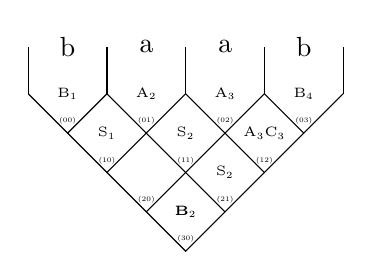
\begin{tikzpicture}[baseline]
							\newcommand{\myfontvars}[1]{
								\fontsize{4.9}{12}\selectfont{#1}
							}\newcommand{\myfontnumbering}[1]{
								\fontsize{2.5}{12}\selectfont{#1}
							}%Outer hull
							%Tip of the pyramid
							\coordinate (tip) at (2.0,-2.0);
							\foreach \i in {0,...,4} {
								\coordinate (\i) at (\i,0);
							}
							%Draw the left and right line of the pyramid pointing downwards
							\draw (0) -- (tip) -- (4);
							%Grid lines direction down-left to top-right
							\coordinate (dl1) at (0.5,-0.5);
							\coordinate (dl2) at (1.0,-1.0);
							\coordinate (dl3) at (1.5,-1.5);
							\draw (dl1) -- (1,0);
							\draw (dl2) -- (2,0);
							\draw (dl3) -- (3,0);
							%Grid lines direction down-right to top-left
							\coordinate (dr1) at (2.5,-1.5);
							\coordinate (dr2) at (3.0,-1.0);
							\coordinate (dr3) at (3.5,-0.5);
							\draw (dr1) -- (1,0);
							\draw (dr2) -- (2,0);
							\draw (dr3) -- (3,0);
							%Small lines at the top
							\coordinate (top0) at (0.0,0.0);
							\coordinate (top1) at (1.0,0.0);
							\coordinate (top2) at (2.0,0.0);
							\coordinate (top3) at (3.0,0.0);
							\coordinate (top4) at (4.0,0.0);
							\coordinate (topUpper0) at (0.0,0.6);
							\coordinate (topUpper1) at (1.0,0.6);
							\coordinate (topUpper2) at (2.0,0.6);
							\coordinate (topUpper3) at (3.0,0.6);
							\coordinate (topUpper4) at (4.0,0.6);
							\draw (top0) -- (topUpper0);
							\draw (top1) -- (topUpper1);
							\draw (top2) -- (topUpper2);
							\draw (top3) -- (topUpper3);
							\draw (top4) -- (topUpper4);
							%The string
							\coordinate (w0) at (0.5,0.6);
							\coordinate (w1) at (1.5,0.6);
							\coordinate (w2) at (2.5,0.6);
							\coordinate (w3) at (3.5,0.6);
							\node [] at (w0) {b};
							\node [] at (w1) {a};
							\node [] at (w2) {a};
							\node [] at (w3) {b};
							% Variables in the cells
							%cells00
							\coordinate (center00) at (0.5,0.0);
							\node [below=0.18cm] at (center00) {\myfontnumbering{$(00)$}};
							\node [] at (center00) {\myfontvars{B$_{1}$}};
							%cells01
							\coordinate (center01) at (1.5,0.0);
							\node [below=0.18cm] at (center01) {\myfontnumbering{$(01)$}};
							\node [] at (center01) {\myfontvars{A$_{2}$}};
							%cells02
							\coordinate (center02) at (2.5,0.0);
							\node [below=0.18cm] at (center02) {\myfontnumbering{$(02)$}};
							\node [] at (center02) {\myfontvars{A$_{3}$}};
							%cells03
							\coordinate (center03) at (3.5,0.0);
							\node [below=0.18cm] at (center03) {\myfontnumbering{$(03)$}};
							\node [] at (center03) {\myfontvars{B$_{4}$}};
							%cells10
							\coordinate (center10) at (1.0,-0.5);
							\node [below=0.18cm] at (center10) {\myfontnumbering{$(10)$}};
							\node [] at (center10) {\myfontvars{S$_{1}$}};
							%cells11
							\coordinate (center11) at (2.0,-0.5);
							\node [below=0.18cm] at (center11) {\myfontnumbering{$(11)$}};
							\node [] at (center11) {\myfontvars{S$_{2}$}};
							%cells12
							\coordinate (center12) at (3.0,-0.5);
							\node [below=0.18cm] at (center12) {\myfontnumbering{$(12)$}};
							\node [] at (center12) {\myfontvars{A$_{3}$C$_{3}$}};
							%cells20
							\coordinate (center20) at (1.5,-1.0);
							\node [below=0.18cm] at (center20) {\myfontnumbering{$(20)$}};
							%cells21
							\coordinate (center21) at (2.5,-1.0);
							\node [below=0.18cm] at (center21) {\myfontnumbering{$(21)$}};
							\node [] at (center21) {\myfontvars{S$_{2}$}};
							%cells30
							\coordinate (center30) at (2.0,-1.5);
							\node [below=0.18cm] at (center30) {\myfontnumbering{$(30)$}};
							\node [] at (center30) {\myfontvars{{\textbf{B$_{2}$}}}};
							\end{tikzpicture}
						}	
					}
				} 
	\end{minipage}
\captionof{figure}{Example of Algorithm \ref{CalculateSubsetForCell} while applying it on $Cell_{3,0}$ via adding the rule $B \rightarrow SC$.}
\noindent The calculation of CellSet for $Cell_{3,0}$ results in $\{SA,~SC,~BS\}$, whereas $SA$ and $SC$ stem from $Cell_{1,0}$ together with $Cell_{1,2}$ and $BA$ comes from $Cell_{0,0}$ together with $Cell_{2,1}$. Now if either one of the rules $lhse \rightarrow SA$, $lhse \rightarrow SC$ or  $lhse \rightarrow BS$ is added to the grammar, then $lhse\in Cell_{3,0}$. Here the rule  \textbf{B $\rightarrow$ SC} has been added and finally $(B,2)$ is element of $Cell_{3,0}$.
\end{testexample}
In general if for one $Cell_{i,j}$ a rule like $lhse \rightarrow cs$ with $cs \in CellSet$ (Line~\ref{cellSet}) is added, then automatically $Cell_{i,j}$ will not be empty any more.

\pagebreak

\subsection{Dice rolling the distributions only} \label{diceRollOnlyCYK}
\noindent We start off by a primitive way of generating grammars, which will be the lower boundary while comparing the algorithms. Note that later on in Chapter \ref{successRates} it is described what "performing better" means in the context of this thesis. \\

\noindent
\frame{
	\begin{algorithm}[H] %or another one check
		\caption{DiceRollOnlyCYK}
		\label{DiceRollOnlyCYK}
		\SetAlgoLined
		\KwIn{Word $w \in \Sigma^{*}$ }
		\KwOut{Set of productions $P$}
		$P = \emptyset$;~~\tcp{$P \subseteq V \times (V^{2} \cup \Sigma)$}
		$P \cup Distribute(\Sigma,\ V)$;  \circled{A}\\ \label{diceRollOnlyA}
		$P \cup Distribute(V^2,\ V)$;  \circled{B}\\ \label{diceRollOnlyB}
		\Return $P$;
	\end{algorithm}
}

\noindent The algoritm DiceRollOnly (Algorithm \ref{DiceRollOnlyCYK}) distributes terminals $\Sigma$ to at least one $lhse$, but a compound variable $vc \in V^2$ does not has to be distributed at all. Note that for each terminal of $\Sigma=\{a,b\}$ at least one rule like $lhse\rightarrow a$ and $lhse\rightarrow b$ is generated.\\

\begin{testexample}[Algorithm DiceRollOnlyCYK]
	For each possible compound variable $V^2=\{AA,~AB,~AC,~AS,~BB,~BC,~BS,~$ $CC,$ $CS,SS\}$ it is possible that only a smaller subset like $\{AA,~BA,~CC,~SC\}$ is distributed (Figure \ref{DiceRollONlyCYKExample}) so that only rules like $lhse\rightarrow AA$, $lhse\rightarrow BA$, $lhse\rightarrow CC$ and $lhse\rightarrow SC$ exist.\\
	\begin{minipage}{6in}
		\centering
		\raisebox{-0.5\height}{
			\begin{tabular}{l}
				Grammar after Line 2:\\
				$C\rightarrow a$\\ 
				$B\rightarrow b$\\
				\\
			\end{tabular} 
			\begin{tabular}{l}
				Grammar after Line 3:\\
				$C\rightarrow BA~|~AA~|~a$\\ 
				$B\rightarrow b$ \\
				$S\rightarrow CC~|~SC$ 
			\end{tabular}
		} 	
	\end{minipage}
	\captionof{figure}{Shortend overview of the example of Algorithm \ref{DiceRollOnlyCYK}.}
	\label{DiceRollONlyCYKExample}
\end{testexample}



\pagebreak
\clearpage
\subsection{Dice rolling and Bottom-Up variant one} \label{var1}
Another approach to design an algorithm is after the Bottom-Up approach (Chapter \ref{approaches}) in which the parsing table is filled starting from the leaves in direction of the root node.\\
The basic idea is to guide the choice of rules while distributing the compound variables $V^2$. In Algorithm \ref{DiceRollOnlyCYK}, the naive approach, it is possible that the terminals are distributed to the variables $A$ and $B$ and Algorithm \ref{DiceRollOnlyCYK} completely discards this fact during the distribution of the compound variables (see Figure \ref{var1ExampleMiddle} in the middle). \\

\begin{testexample}[Disregarding already added rules]
	Figure \ref{var1ExampleTop} shows the starting situation for this example.
	
		\centering
				\raisebox{-0.5\height}{
			\begin{tabular}{l}
				Grammar:\\
				$A\rightarrow a$\\
				$B \rightarrow b$\\ 
			\end{tabular} 
		}
		\hspace*{.2in}
		\resizebox{0.5\linewidth}{!}{
			\resizebox{\linewidth}{!}{
				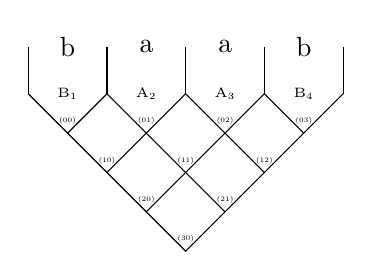
\begin{tikzpicture}[baseline]
				\newcommand{\myfontvars}[1]{
					\fontsize{4.9}{12}\selectfont{#1}
				}\newcommand{\myfontnumbering}[1]{
					\fontsize{2.5}{12}\selectfont{#1}
				}%Outer hull
				%Tip of the pyramid
				\coordinate (tip) at (2.0,-2.0);
				\foreach \i in {0,...,4} {
					\coordinate (\i) at (\i,0);
				}
				%Draw the left and right line of the pyramid pointing downwards
				\draw (0) -- (tip) -- (4);
				%Grid lines direction down-left to top-right
				\coordinate (dl1) at (0.5,-0.5);
				\coordinate (dl2) at (1.0,-1.0);
				\coordinate (dl3) at (1.5,-1.5);
				\draw (dl1) -- (1,0);
				\draw (dl2) -- (2,0);
				\draw (dl3) -- (3,0);
				%Grid lines direction down-right to top-left
				\coordinate (dr1) at (2.5,-1.5);
				\coordinate (dr2) at (3.0,-1.0);
				\coordinate (dr3) at (3.5,-0.5);
				\draw (dr1) -- (1,0);
				\draw (dr2) -- (2,0);
				\draw (dr3) -- (3,0);
				%Small lines at the top
				\coordinate (top0) at (0.0,0.0);
				\coordinate (top1) at (1.0,0.0);
				\coordinate (top2) at (2.0,0.0);
				\coordinate (top3) at (3.0,0.0);
				\coordinate (top4) at (4.0,0.0);
				\coordinate (topUpper0) at (0.0,0.6);
				\coordinate (topUpper1) at (1.0,0.6);
				\coordinate (topUpper2) at (2.0,0.6);
				\coordinate (topUpper3) at (3.0,0.6);
				\coordinate (topUpper4) at (4.0,0.6);
				\draw (top0) -- (topUpper0);
				\draw (top1) -- (topUpper1);
				\draw (top2) -- (topUpper2);
				\draw (top3) -- (topUpper3);
				\draw (top4) -- (topUpper4);
				%The string
				\coordinate (w0) at (0.5,0.6);
				\coordinate (w1) at (1.5,0.6);
				\coordinate (w2) at (2.5,0.6);
				\coordinate (w3) at (3.5,0.6);
				\node [] at (w0) {b};
				\node [] at (w1) {a};
				\node [] at (w2) {a};
				\node [] at (w3) {b};
				% Variables in the cells
				%cells00
				\coordinate (center00) at (0.5,0.0);
				\node [below=0.18cm] at (center00) {\myfontnumbering{$(00)$}};
				\node [] at (center00) {\myfontvars{B$_{1}$}};
				%cells01
				\coordinate (center01) at (1.5,0.0);
				\node [below=0.18cm] at (center01) {\myfontnumbering{$(01)$}};
				\node [] at (center01) {\myfontvars{A$_{2}$}};
				%cells02
				\coordinate (center02) at (2.5,0.0);
				\node [below=0.18cm] at (center02) {\myfontnumbering{$(02)$}};
				\node [] at (center02) {\myfontvars{A$_{3}$}};
				%cells03
				\coordinate (center03) at (3.5,0.0);
				\node [below=0.18cm] at (center03) {\myfontnumbering{$(03)$}};
				\node [] at (center03) {\myfontvars{B$_{4}$}};
				%cells10
				\coordinate (center10) at (1.0,-0.5);
				\node [below=0.18cm] at (center10) {\myfontnumbering{$(10)$}};
				%cells11
				\coordinate (center11) at (2.0,-0.5);
				\node [below=0.18cm] at (center11) {\myfontnumbering{$(11)$}};
				%cells12
				\coordinate (center12) at (3.0,-0.5);
				\node [below=0.18cm] at (center12) {\myfontnumbering{$(12)$}};
				%cells20
				\coordinate (center20) at (1.5,-1.0);
				\node [below=0.18cm] at (center20) {\myfontnumbering{$(20)$}};
				%cells21
				\coordinate (center21) at (2.5,-1.0);
				\node [below=0.18cm] at (center21) {\myfontnumbering{$(21)$}};
				%cells30
				\coordinate (center30) at (2.0,-1.5);
				\node [below=0.18cm] at (center30) {\myfontnumbering{$(30)$}};
				\end{tikzpicture}
			}	
		}
		\captionof{figure}{Disregarding the already added rules: Starting situation.}
	    \label{var1ExampleTop}
	    
	   \justify If rules like $lhse \rightarrow CC$ or $lhse \rightarrow SC$ are added they do not directly help to fill the parsing table and bloat the grammar with useless rules (see Figure \ref{var1ExampleMiddle}). This is a unfortunate adding of rules that does not help to fill the parsing table and can happen in Algorithm \ref{DiceRollOnlyCYK}.
	   
	   \centering
		\begin{minipage}{6in}
			\centering
			\raisebox{-0.5\height}{
				\begin{tabular}{l}
					Grammar:\\
					$A\rightarrow \mathbf{CC}~|~a$\\
					$B \rightarrow b$\\ 
				\end{tabular} 
			}
			\hspace*{.2in}
			\resizebox{0.5\linewidth}{!}{
				\resizebox{\linewidth}{!}{
					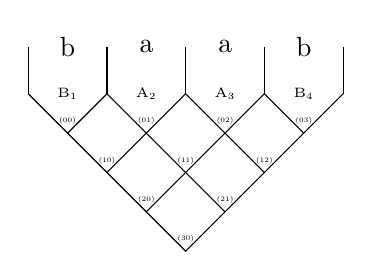
\begin{tikzpicture}[baseline]
					\newcommand{\myfontvars}[1]{
						\fontsize{4.9}{12}\selectfont{#1}
					}\newcommand{\myfontnumbering}[1]{
						\fontsize{2.5}{12}\selectfont{#1}
					}%Outer hull
					%Tip of the pyramid
					\coordinate (tip) at (2.0,-2.0);
					\foreach \i in {0,...,4} {
						\coordinate (\i) at (\i,0);
					}
					%Draw the left and right line of the pyramid pointing downwards
					\draw (0) -- (tip) -- (4);
					%Grid lines direction down-left to top-right
					\coordinate (dl1) at (0.5,-0.5);
					\coordinate (dl2) at (1.0,-1.0);
					\coordinate (dl3) at (1.5,-1.5);
					\draw (dl1) -- (1,0);
					\draw (dl2) -- (2,0);
					\draw (dl3) -- (3,0);
					%Grid lines direction down-right to top-left
					\coordinate (dr1) at (2.5,-1.5);
					\coordinate (dr2) at (3.0,-1.0);
					\coordinate (dr3) at (3.5,-0.5);
					\draw (dr1) -- (1,0);
					\draw (dr2) -- (2,0);
					\draw (dr3) -- (3,0);
					%Small lines at the top
					\coordinate (top0) at (0.0,0.0);
					\coordinate (top1) at (1.0,0.0);
					\coordinate (top2) at (2.0,0.0);
					\coordinate (top3) at (3.0,0.0);
					\coordinate (top4) at (4.0,0.0);
					\coordinate (topUpper0) at (0.0,0.6);
					\coordinate (topUpper1) at (1.0,0.6);
					\coordinate (topUpper2) at (2.0,0.6);
					\coordinate (topUpper3) at (3.0,0.6);
					\coordinate (topUpper4) at (4.0,0.6);
					\draw (top0) -- (topUpper0);
					\draw (top1) -- (topUpper1);
					\draw (top2) -- (topUpper2);
					\draw (top3) -- (topUpper3);
					\draw (top4) -- (topUpper4);
					%The string
					\coordinate (w0) at (0.5,0.6);
					\coordinate (w1) at (1.5,0.6);
					\coordinate (w2) at (2.5,0.6);
					\coordinate (w3) at (3.5,0.6);
					\node [] at (w0) {b};
					\node [] at (w1) {a};
					\node [] at (w2) {a};
					\node [] at (w3) {b};
					% Variables in the cells
					%cells00
					\coordinate (center00) at (0.5,0.0);
					\node [below=0.18cm] at (center00) {\myfontnumbering{$(00)$}};
					\node [] at (center00) {\myfontvars{B$_{1}$}};
					%cells01
					\coordinate (center01) at (1.5,0.0);
					\node [below=0.18cm] at (center01) {\myfontnumbering{$(01)$}};
					\node [] at (center01) {\myfontvars{A$_{2}$}};
					%cells02
					\coordinate (center02) at (2.5,0.0);
					\node [below=0.18cm] at (center02) {\myfontnumbering{$(02)$}};
					\node [] at (center02) {\myfontvars{A$_{3}$}};
					%cells03
					\coordinate (center03) at (3.5,0.0);
					\node [below=0.18cm] at (center03) {\myfontnumbering{$(03)$}};
					\node [] at (center03) {\myfontvars{B$_{4}$}};
					%cells10
					\coordinate (center10) at (1.0,-0.5);
					\node [below=0.18cm] at (center10) {\myfontnumbering{$(10)$}};
					%cells11
					\coordinate (center11) at (2.0,-0.5);
					\node [below=0.18cm] at (center11) {\myfontnumbering{$(11)$}};
					%cells12
					\coordinate (center12) at (3.0,-0.5);
					\node [below=0.18cm] at (center12) {\myfontnumbering{$(12)$}};
					%cells20
					\coordinate (center20) at (1.5,-1.0);
					\node [below=0.18cm] at (center20) {\myfontnumbering{$(20)$}};
					%cells21
					\coordinate (center21) at (2.5,-1.0);
					\node [below=0.18cm] at (center21) {\myfontnumbering{$(21)$}};
					%cells30
					\coordinate (center30) at (2.0,-1.5);
					\node [below=0.18cm] at (center30) {\myfontnumbering{$(30)$}};
					\end{tikzpicture}
				}	
			}
		\end{minipage}
	\captionof{figure}{Disregarding the already added rules middle: Unfortunate adding. Bottom: Advantageous adding of rules.}
	\label{var1ExampleMiddle}
	
	\justify More reasonable rules to add would be $lhse \rightarrow BA$, $lhse \rightarrow AA$ or $lhse \rightarrow AB$ (see Figure \ref{var1ExampleDown}). This is an advantageous adding of rules as intended in Algorithm \ref{BottomUpDiceRollVar1} that helps to fill the $pyramid$.
	
	\centering
		\begin{minipage}{6in}
			\centering
			\raisebox{-0.5\height}{
				\begin{tabular}{l}
					Grammar:\\
					$A\rightarrow a$\\
					$B \rightarrow \mathbf{AB}~|~b$\\ 
				\end{tabular} 
			}
			\hspace*{.2in}
			\resizebox{0.5\linewidth}{!}{
				\resizebox{\linewidth}{!}{
					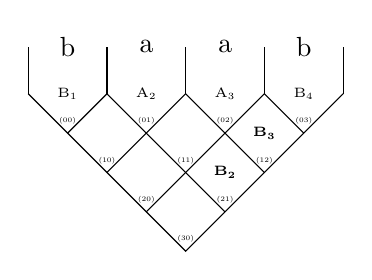
\begin{tikzpicture}[baseline]
					\newcommand{\myfontvars}[1]{
						\fontsize{4.9}{12}\selectfont{#1}
					}\newcommand{\myfontnumbering}[1]{
						\fontsize{2.5}{12}\selectfont{#1}
					}%Outer hull
					%Tip of the pyramid
					\coordinate (tip) at (2.0,-2.0);
					\foreach \i in {0,...,4} {
						\coordinate (\i) at (\i,0);
					}
					%Draw the left and right line of the pyramid pointing downwards
					\draw (0) -- (tip) -- (4);
					%Grid lines direction down-left to top-right
					\coordinate (dl1) at (0.5,-0.5);
					\coordinate (dl2) at (1.0,-1.0);
					\coordinate (dl3) at (1.5,-1.5);
					\draw (dl1) -- (1,0);
					\draw (dl2) -- (2,0);
					\draw (dl3) -- (3,0);
					%Grid lines direction down-right to top-left
					\coordinate (dr1) at (2.5,-1.5);
					\coordinate (dr2) at (3.0,-1.0);
					\coordinate (dr3) at (3.5,-0.5);
					\draw (dr1) -- (1,0);
					\draw (dr2) -- (2,0);
					\draw (dr3) -- (3,0);
					%Small lines at the top
					\coordinate (top0) at (0.0,0.0);
					\coordinate (top1) at (1.0,0.0);
					\coordinate (top2) at (2.0,0.0);
					\coordinate (top3) at (3.0,0.0);
					\coordinate (top4) at (4.0,0.0);
					\coordinate (topUpper0) at (0.0,0.6);
					\coordinate (topUpper1) at (1.0,0.6);
					\coordinate (topUpper2) at (2.0,0.6);
					\coordinate (topUpper3) at (3.0,0.6);
					\coordinate (topUpper4) at (4.0,0.6);
					\draw (top0) -- (topUpper0);
					\draw (top1) -- (topUpper1);
					\draw (top2) -- (topUpper2);
					\draw (top3) -- (topUpper3);
					\draw (top4) -- (topUpper4);
					%The string
					\coordinate (w0) at (0.5,0.6);
					\coordinate (w1) at (1.5,0.6);
					\coordinate (w2) at (2.5,0.6);
					\coordinate (w3) at (3.5,0.6);
					\node [] at (w0) {b};
					\node [] at (w1) {a};
					\node [] at (w2) {a};
					\node [] at (w3) {b};
					% Variables in the cells
					%cells00
					\coordinate (center00) at (0.5,0.0);
					\node [below=0.18cm] at (center00) {\myfontnumbering{$(00)$}};
					\node [] at (center00) {\myfontvars{B$_{1}$}};
					%cells01
					\coordinate (center01) at (1.5,0.0);
					\node [below=0.18cm] at (center01) {\myfontnumbering{$(01)$}};
					\node [] at (center01) {\myfontvars{A$_{2}$}};
					%cells02
					\coordinate (center02) at (2.5,0.0);
					\node [below=0.18cm] at (center02) {\myfontnumbering{$(02)$}};
					\node [] at (center02) {\myfontvars{A$_{3}$}};
					%cells03
					\coordinate (center03) at (3.5,0.0);
					\node [below=0.18cm] at (center03) {\myfontnumbering{$(03)$}};
					\node [] at (center03) {\myfontvars{B$_{4}$}};
					%cells10
					\coordinate (center10) at (1.0,-0.5);
					\node [below=0.18cm] at (center10) {\myfontnumbering{$(10)$}};
					%cells11
					\coordinate (center11) at (2.0,-0.5);
					\node [below=0.18cm] at (center11) {\myfontnumbering{$(11)$}};
					%cells12
					\coordinate (center12) at (3.0,-0.5);
					\node [below=0.18cm] at (center12) {\myfontnumbering{$(12)$}};
					\node [] at (center12) {\myfontvars{\textbf{B}$\mathbf{_{3}}$}};
					%cells20
					\coordinate (center20) at (1.5,-1.0);
					\node [below=0.18cm] at (center20) {\myfontnumbering{$(20)$}};
					%cells21
					\coordinate (center21) at (2.5,-1.0);
					\node [below=0.18cm] at (center21) {\myfontnumbering{$(21)$}};
					\node [] at (center21) {\myfontvars{\textbf{B}$\mathbf{_{2}}$}};
					%cells30
					\coordinate (center30) at (2.0,-1.5);
					\node [below=0.18cm] at (center30) {\myfontnumbering{$(30)$}};
					\end{tikzpicture}
				}	
			}
		\end{minipage}	
\captionof{figure}{Disregarding the already added rules Bottom: Advantageous adding of rules.}
\label{var1ExampleDown}
\end{testexample}
\pagebreak
\noindent Algorithm \ref{BottomUpDiceRollVar1} continues on this idea: After distributing the terminals (Line \ref{distrTerm}) the updated parsing table (Line \ref{var1Update}) is always taken into consideration while calculating (Line \ref{var1D}) variable compounds and to finally add a part of them (Line \ref{var1Add}) in form of rules to the grammar. As explanation, for each chosen cell a $CellSet$ (Line \ref{var1D}) is calculated, that only contains reasonable variable compounds. This way only variable compounds are added that directly help to fill the parsing table.\\

\noindent
\frame{
	\begin{algorithm}[H] %or another one check
		\caption{BottomUpDiceRollVar1}
		\label{BottomUpDiceRollVar1}
		\SetAlgoLined
		\KwIn{Word $w \in \Sigma^{*}$ }
		\KwOut{Set of productions $P$}
		$P = \emptyset$;~~\tcp{$P \subseteq V \times (V^{2} \cup \Sigma)$}
		$P = Distribute(\Sigma,\ V)$;  \circled{A} \label{distrTerm}\\
		$Pyramid = CYK(G,\ w)$\label{var1Stepii}\;
		\For{$i:=1\ \textbf{to}\ i_{max}$}{
			$J = \{0,~...~,~j_{max} -1\}$;~~\tcp{$J \subseteq \mathbb{N}$}
			$CellSet = \emptyset$;~~\tcp{$CellSet \subseteq V^2$} \label{var1A}
			\While{$|J|>0$}{
				$choose\ one\ j \in J\ uniform\ randomly$\;
				$J = J \setminus \{j\} $\label{chooseJ}\;
				$CellSet = CalculateSubsetForCell(Pyramid,\ i,\ j)$;  \circled{D} \label{var1D}\\
				$P \cup Distribute(CellSet,\ V)$;  \circled{B} \label{var1Add}\\
				$Pyramid = CYK(G,\ w)$\; \label{var1Update}
				\If{$stopping\ criteria~met$~\circled{C}}{
					\Return $P$\;
				}
			}
		}
		\Return $P$\;
		\footnotetext{
			\noindent Line \ref{var1Stepii}: Fills the i=0 row of the pyramid.
			\noindent Line \ref{chooseJ}: A cell is visited only once.
		}
	\end{algorithm}
}

\pagebreak
\subsection{Dice rolling and Bottom-Up variant two} \label{var2}
While examining Algorithm \ref{BottomUpDiceRollVar1} via its log file (Figure \ref{logsVar1}) it can be seen that already a very small number of rules in the grammar is sufficient so that the stopping criteria \circled{C} is met \textendash~the cells that indirectly decide what rules to add are mostly from row one ($i=1$) and sometimes if at all from row two ($i=2$).\\

\begin{figure}[h]
	\centering
		\begin{tabular}{l}
			Final cell worked with Index: 1,2\\
			Final cell worked with Index: 1,0\\
			Final cell worked with Index: 1,6 \\
			Final cell worked with Index: 1,0\\
			Final cell worked with Index: 1,2\\
			Final cell worked with Index: 1,3\\
			Final cell worked with Index: 2,4\\
	\end{tabular}
	\caption{Overview of log files of Algorithm \ref{BottomUpDiceRollVar1} with $|V|=4$ and $|\Sigma|=2$.}
	\label{logsVar1}
\end{figure}
\noindent This again leads to a further improvement idea to introduce a row dependent $threshold_i$ (Line \ref{var2threshold} of Algorithm \ref{BottomUpDiceRollVar2} BottomUpDiceRollVars) which helps that more cells with $i\geq2$ are chosen \textendash~what possibly leads to more diverse grammars being generated. The diversity, in context of the procedure BottomUpDiceRollVar1 (Algorithm \ref{BottomUpDiceRollVar1}), is somewhat too restricted to the $lhse$s that have one of the terminals as its $rhse$. Most of the rules that are part of the grammar will contain one of these $lhse$s as explained in Chapter \ref{var1}. This is caused by the basic idea of Algorithm \ref{BottomUpDiceRollVar1} but also due to the relatively small number of rules that are added to the grammar altogether. \\
Further diversification is achieved through the usage of \circled{E} (Line \ref{chooseVc} of Algorithm \ref{BottomUpDiceRollVar2} BottomUpDiceRollVars), i.e. the variable compounds that already have been used in a row with low index $i$ are at a disadvantage to be picked again (A more detailed explanation is found at the and of this chapter).\\

\begin{testexample}[Better diversity in a grammar]
	As seen in Figure \ref{GoalofBetterDiversity} the rules with $BA$~and~$AA$ are added to the variables $B$ and $A$ in Grammar1. For Grammar2 instead the rule $B\rightarrow SS$ is added that contributes to a better diversity compared to Grammar1. Grammar2 contains one more unique $rhse$ ($SS$) compared to Grammar1.\\
	
	\begin{minipage}{6in}
		\centering
		\raisebox{-0.5\height}{
			\begin{tabular}{l}
				Grammar0:\\
				$C\rightarrow BA~|~AA~|~a$\\ 
				$B\rightarrow b$ \\
				$S\rightarrow CC~|~SC$ 
			\end{tabular}
			\begin{tabular}{l}
				Grammar1:\\
				$C\rightarrow BA~|~AA~|~a$\\ 
				$B\rightarrow BA~|~AA~|~b$ \\
				$S\rightarrow BA~|~AA~|~CC~|~SC$ 
			\end{tabular}
			\begin{tabular}{l}
				Grammar2:\\
				$C\rightarrow BA~|~AA~|~a$\\ 
				$B\rightarrow SS~|~b$ \\
				$S\rightarrow CC~|~SC$ 
			\end{tabular}
		} 
	\end{minipage}
	\captionof{figure}{Better diversity.: Starting point is Grammar0 and Grammar2 is of better diversity than Grammar1.}
	\label{GoalofBetterDiversity}
\end{testexample}

\noindent
\frame{
	\begin{algorithm}[H] %or another one check
		\caption{BottomUpDiceRollVar2}
		\label{BottomUpDiceRollVar2}
		\SetAlgoLined
		\KwIn{Word $w \in \Sigma^{*}$ }
		\KwOut{Set of productions $P$}
		$P = \emptyset$;~~\tcp{$P \subseteq V \times (V^{2} \cup \Sigma)$}
		$RowSet = \emptyset$;~~\tcp{$RowSet \subseteq \{(xy,i)\ |\ x,y \in V \wedge i \in \mathbb{N} \}$}
		$P = Distribute(\Sigma,\ V)$;  \circled{A}\\
		$Pyramid = CYK(G,\ w)$ \label{stepii}\;
		\For{$i:=1\ \textbf{to}\ i_{max}$}{
			%$choose\ j\ uniform\ randomly\ in\ [0,\ j_{max}-i]  $\;
			\For{$j:=0\ \textbf{to}\ j_{max}-i$}{
				$RowSet \cup \{(xy,i)\ |\ xy \in CalculateSubsetForCell(Pyramid,\ i,\ j) $\circled{D}$\}$\label{rowSet}\;  
			}
			\While{$threshold_i\ not\ reached $}{ \label{var2threshold}
				$choose~ one~ (xy,\ i)~ from~ RowSet~ uniform\ randomly\ with$ $probability~depending~on~i $;\label{chooseVc} \circled{E}  \\
				$P \cup Distribute(xy,\ V) $; \circled{B}  \\
				$Pyramid = CYK(G,\ w)$\;
				\If{$stopping\ criteria~met$~\circled{C}}{
					\Return $P$\;
				}	
			}
		}
		\Return $P$\;
		\footnotetext{
			\noindent Line \ref{stepii}: Fills the i=0 row of the pyramid.
		}
	\end{algorithm}
}
~

\noindent \textbf{Choose one xy from (xy,i) $\in$ RowSet uniform randomly with probability depending on row i \circled{E} :}\\
At some point a decision needs to me made about what rule $lhse\rightarrow xy$ with $xy \in V^2$ will be added to the grammar. Depending on which $xy$ is chosen the influence on the entire pyramid varies. Some $xy$ only change the parsing table in one of its later rows ($i>>1$) but other $xy$ even change it in one of the first rows. If there is a change in one of the first rows it is more likely that the entire pyramid will be filled with more elements. Now the task of choosing rules to add, that only change the pyramid in one of the later rows, with a higher probability than the others is tackled with \circled{E}. \\
The approach here only makes sense together with \circled{D} in which all possible compound variables are calculated that help to fill one specific cell. $RowSet \subseteq \{(xy,i)\ |\ x,y \in V \wedge i \in \mathbb{N} \}$ whereas the $xy$ are calculated with \circled{D} and $i$ is the row number of the specific cell. \pagebreak \clearpage

\begin{testexample}[Procedure \circled{E}]
	With $RowSet$ the choice can be influenced regarding the row number $i$: Firstly the $RowSet$ is compressed, i.e. every tuple with the same $xy$ will be merged to its lowest $i$, as following: $RowSet = \{(AB,3),~(AB,1),~(AB,5),~... \}$ will become $RowSet = \{(AB,1),~... \}$. Afterwards all elements of $RowSet$ will be placed in the $RowMultiSet$ that  can contain multiple equivalent elements. Now each element of $RowMultiSet$ will be weighted according to their $i$. That means that elements like $(AB,1)$ will only occur one time while elements like $(BC,3)$ will occur three times and so on: $RowMultiSet = \{(AB,1),~(BC,3),~...\}$ becomes $RowMultiSet = \{(AB,1),~(BC,3),~(BC,3),~(BC,3),~...\}$. Now one element will be chosen uniformly randomly out of this weighted $RowMultiSet$. In the example in Figure \ref{exampleProcE} this results in $xy = BC$.\\
	
	\begin{minipage}{6in}
		\centering
		\raisebox{-0.5\height}{
			\begin{tabular}{l l}
				$RowSet = \{(AB,3),(AB,1),(AB,5),... \}$ & // compress \\
				$RowSet = \{(AB,1),... \}$ & // put in RowMultiSet \\
				$RowMultiSet = \{(AB,1),(BC,3),...\}$ & // weight elements \\
				$RowMultiSet = \{(AB,1),(BC,3),(BC,3),(BC,3),...\}$ & // pick element\\
				$xy = BC$
			\end{tabular} 
		} 		
	\end{minipage}
	\captionof{figure}{Overview of the procedure E.}
	\label{exampleProcE}
\end{testexample}

\pagebreak
\subsection{Split Top-Down and fill Bottom-Up}
Until now we have only discussed algorithms that purely use the Bottom-Up approach, so another way is to utilize the Top-Down approach in combination with the Bottom-Up approach.\\
The idea here is first to distribute the terminals (Line \ref{splitThenStepii} of Algorithm \ref{SplitThenFill} SplitThenFill) and then to uniformly randomly generate a predefined structure of the derivation tree (Line \ref{splitThenFillTreeStart} of Algorithm \ref{SplitThenFill} and in general Algorithm \ref{SplitThenFillRecursion} SplitThenFillRec) Top-Downwards and then again to fill the parsing table Bottom-Upwards accordingly to fill this derivation tree. The structure of the derivation tree for instance can look as follows:\\

\begin{testexample}[Derivation structure in the pyramid and as a derivation tree]
	The numbers correspond to the depth in the tree.\\
	\begin{minipage}{6in}
		\centering
		\resizebox{0.8\linewidth}{!}{
			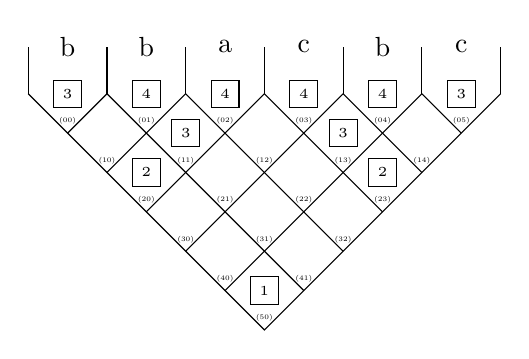
\begin{tikzpicture}[baseline]
			\newcommand{\myfontvars}[1]{
				\fontsize{4.9}{12}\selectfont{#1}
			}\newcommand{\myfontnumbering}[1]{
				\fontsize{2.5}{12}\selectfont{#1}
			}%Outer hull
			%Tip of the pyramid
			\coordinate (tip) at (3.0,-3.0);
			\foreach \i in {0,...,6} {
				\coordinate (\i) at (\i,0);
			}
			%Draw the left and right line of the pyramid pointing downwards
			\draw (0) -- (tip) -- (6);
			%Grid lines direction down-left to top-right
			\coordinate (dl1) at (0.5,-0.5);
			\coordinate (dl2) at (1.0,-1.0);
			\coordinate (dl3) at (1.5,-1.5);
			\coordinate (dl4) at (2.0,-2.0);
			\coordinate (dl5) at (2.5,-2.5);
			\draw (dl1) -- (1,0);
			\draw (dl2) -- (2,0);
			\draw (dl3) -- (3,0);
			\draw (dl4) -- (4,0);
			\draw (dl5) -- (5,0);
			%Grid lines direction down-right to top-left
			\coordinate (dr1) at (3.5,-2.5);
			\coordinate (dr2) at (4.0,-2.0);
			\coordinate (dr3) at (4.5,-1.5);
			\coordinate (dr4) at (5.0,-1.0);
			\coordinate (dr5) at (5.5,-0.5);
			\draw (dr1) -- (1,0);
			\draw (dr2) -- (2,0);
			\draw (dr3) -- (3,0);
			\draw (dr4) -- (4,0);
			\draw (dr5) -- (5,0);
			%Small lines at the top
			\coordinate (top0) at (0.0,0.0);
			\coordinate (top1) at (1.0,0.0);
			\coordinate (top2) at (2.0,0.0);
			\coordinate (top3) at (3.0,0.0);
			\coordinate (top4) at (4.0,0.0);
			\coordinate (top5) at (5.0,0.0);
			\coordinate (top6) at (6.0,0.0);
			\coordinate (topUpper0) at (0.0,0.6);
			\coordinate (topUpper1) at (1.0,0.6);
			\coordinate (topUpper2) at (2.0,0.6);
			\coordinate (topUpper3) at (3.0,0.6);
			\coordinate (topUpper4) at (4.0,0.6);
			\coordinate (topUpper5) at (5.0,0.6);
			\coordinate (topUpper6) at (6.0,0.6);
			\draw (top0) -- (topUpper0);
			\draw (top1) -- (topUpper1);
			\draw (top2) -- (topUpper2);
			\draw (top3) -- (topUpper3);
			\draw (top4) -- (topUpper4);
			\draw (top5) -- (topUpper5);
			\draw (top6) -- (topUpper6);
			%The string
			\coordinate (w0) at (0.5,0.6);
			\coordinate (w1) at (1.5,0.6);
			\coordinate (w2) at (2.5,0.6);
			\coordinate (w3) at (3.5,0.6);
			\coordinate (w4) at (4.5,0.6);
			\coordinate (w5) at (5.5,0.6);
			\node [] at (w0) {b};
			\node [] at (w1) {b};
			\node [] at (w2) {a};
			\node [] at (w3) {c};
			\node [] at (w4) {b};
			\node [] at (w5) {c};
			% Variables in the cells
			%cells00
			\coordinate (center00) at (0.5,0.0);
			\node [below=0.18cm] at (center00) {\myfontnumbering{$(00)$}};
			\node [] at (center00) [minimum height=0.25cm,minimum width=0.25cm,draw] {\tiny{3}};
			%cells01
			\coordinate (center01) at (1.5,0.0);
			\node [below=0.18cm] at (center01) {\myfontnumbering{$(01)$}};
			\node [] at (center01) [minimum height=0.25cm,minimum width=0.25cm,draw] {\tiny{4}};
			%cells02
			\coordinate (center02) at (2.5,0.0);
			\node [below=0.18cm] at (center02) {\myfontnumbering{$(02)$}};
			\node [] at (center02) [minimum height=0.25cm,minimum width=0.25cm,draw] {\tiny{4}};
			%cells03
			\coordinate (center03) at (3.5,0.0);
			\node [below=0.18cm] at (center03) {\myfontnumbering{$(03)$}};
			\node [] at (center03) [minimum height=0.25cm,minimum width=0.25cm,draw] {\tiny{4}};
			%cells04
			\coordinate (center04) at (4.5,0.0);
			\node [below=0.18cm] at (center04) {\myfontnumbering{$(04)$}};
			\node [] at (center04) [minimum height=0.25cm,minimum width=0.25cm,draw] {\tiny{4}};
			%cells05
			\coordinate (center05) at (5.5,0.0);
			\node [below=0.18cm] at (center05) {\myfontnumbering{$(05)$}};
			\node [] at (center05) [minimum height=0.25cm,minimum width=0.25cm,draw] {\tiny{3}};
			%cells10
			\coordinate (center10) at (1.0,-0.5);
			\node [below=0.18cm] at (center10) {\myfontnumbering{$(10)$}};
			%cells11
			\coordinate (center11) at (2.0,-0.5);
			\node [below=0.18cm] at (center11) {\myfontnumbering{$(11)$}};
			\node [] at (center11) [minimum height=0.25cm,minimum width=0.25cm,draw] {\tiny{3}};
			%cells12
			\coordinate (center12) at (3.0,-0.5);
			\node [below=0.18cm] at (center12) {\myfontnumbering{$(12)$}};
			%cells13
			\coordinate (center13) at (4.0,-0.5);
			\node [below=0.18cm] at (center13) {\myfontnumbering{$(13)$}};
			\node [] at (center13) [minimum height=0.25cm,minimum width=0.25cm,draw] {\tiny{3}};
			%cells14
			\coordinate (center14) at (5.0,-0.5);
			\node [below=0.18cm] at (center14) {\myfontnumbering{$(14)$}};
			%cells20
			\coordinate (center20) at (1.5,-1.0);
			\node [below=0.18cm] at (center20) {\myfontnumbering{$(20)$}};
			\node [] at (center20) [minimum height=0.25cm,minimum width=0.25cm,draw] {\tiny{2}};
			%cells21
			\coordinate (center21) at (2.5,-1.0);
			\node [below=0.18cm] at (center21) {\myfontnumbering{$(21)$}};
			%cells22
			\coordinate (center22) at (3.5,-1.0);
			\node [below=0.18cm] at (center22) {\myfontnumbering{$(22)$}};
			%cells23
			\coordinate (center23) at (4.5,-1.0);
			\node [below=0.18cm] at (center23) {\myfontnumbering{$(23)$}};
			\node [] at (center23) [minimum height=0.25cm,minimum width=0.25cm,draw] {\tiny{2}};
			%cells30
			\coordinate (center30) at (2.0,-1.5);
			\node [below=0.18cm] at (center30) {\myfontnumbering{$(30)$}};
			%cells31
			\coordinate (center31) at (3.0,-1.5);
			\node [below=0.18cm] at (center31) {\myfontnumbering{$(31)$}};
			%cells32
			\coordinate (center32) at (4.0,-1.5);
			\node [below=0.18cm] at (center32) {\myfontnumbering{$(32)$}};
			%cells40
			\coordinate (center40) at (2.5,-2.0);
			\node [below=0.18cm] at (center40) {\myfontnumbering{$(40)$}};
			%cells41
			\coordinate (center41) at (3.5,-2.0);
			\node [below=0.18cm] at (center41) {\myfontnumbering{$(41)$}};
			%cells50
			\coordinate (center50) at (3.0,-2.5);
			\node [below=0.18cm] at (center50) {\myfontnumbering{$(50)$}};
			\node [] at (center50) [minimum height=0.25cm,minimum width=0.25cm,draw] {\tiny{1}};
			\end{tikzpicture}
		}
		\resizebox{0.70\linewidth}{!}{
			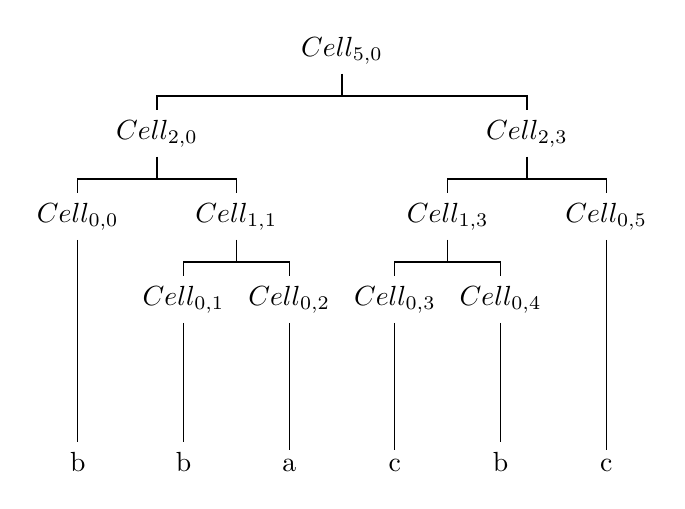
\begin{tikzpicture}[baseline]
			\tikzset{frontier/.style={distance from root=150pt}} %height of tree times 30pt
			\tikzset{edge from parent/.style= {
					draw,
					edge from parent path={(\tikzparentnode.south)	-- +(0,-8pt)-| (\tikzchildnode)}
				}
			}
			\Tree
			[.$Cell_{5,0}$
			[.$Cell_{2,0}$
			[.$Cell_{0,0}$ b ]
			[.$Cell_{1,1}$
			[.$Cell_{0,1}$ b ]
			[.$Cell_{0,2}$ a ]
			]
			]
			[.$Cell_{2,3}$
			[.$Cell_{1,3}$
			[.$Cell_{0,3}$ c ]
			[.$Cell_{0,4}$ b ]
			]
			[.$Cell_{0,5}$ c ]
			]
			]
			\end{tikzpicture}
		}
	\end{minipage}
	\captionof{figure}{Derivation structure shown in the pyramid in the top and down as a derivation tree.}
	\label{treeStruct}
\end{testexample}

\noindent As the name of the algorithms implies only after completely generating the structure of the derivation tree (splitting of the word in sub words) the rules are added to the grammar that help filling the cells occurring in the derivation tree.\\
Now every time before adding a new rule (Algorithm \ref{SplitThenFillRecursion} SplitThenFillRec Line \ref{splitThenFillB}) the already available information regarding the other rules is used to determine if a new rule is needed to fill this node of the derivation tree (Line \ref{empty} of Algorithm \ref{SplitThenFillRecursion} SplitThenFillRec).\\


\noindent
\frame{
	\begin{algorithm}[H] %or another one check
		\caption{SplitThenFill}
		\label{SplitThenFill}
		\SetAlgoLined
		\KwIn{Word $w \in \Sigma^{*}$}
		\KwOut{Set of productions $P$}
		$P = \emptyset$;~~\tcp{$P \subseteq V \times (V^{2} \cup \Sigma)$}
		$P = Distribute(\Sigma,\ V)$; \circled{A} \label{splitThenStepii}  \\		
		$Sol = (P_{Sol},~Cell_{i_{max},0})$;~~\tcp{$P_{Sol} \subseteq P~\wedge~ Cell_{i_{max},0} \in Pyramid$} \label{cell}
		$Sol = SplitThenFillRec(P,\ w,\ i_{max},\ 0)$\; \label{splitThenFillTreeStart}
		\Return $P_{Sol}$\;
		\footnotetext{
			\noindent Line \ref{splitThenStepii}: Fills the i=0 row of the pyramid.	
		}
	\end{algorithm}
}
\\
For this algorithm it is important to mention that while using \circled{B} (Line \ref{splitThenFillB} of Algorithm \ref{SplitThenFillRecursion}) a variable compound is added to at least one $lhse$. For every element of $vc \in VarComp$ (Line \ref{splitThenFillVc} of Algorithm \ref{SplitThenFillRecursion}) there exists at least one rule $lhse \rightarrow vc$.\\

\noindent
\frame{
	\begin{algorithm}[H] %or another one check
		\caption{SplitThenFillRec}
		\label{SplitThenFillRecursion}
		\SetAlgoLined
		\KwIn{$P_{in} \subseteq V \times (V^{2} \cup \Sigma),\ w \in \Sigma^{*},\ i,j \in \mathbb{N}$ }
		\KwOut{$(P,~Cell_{i,j})$}
		$P =  P_{in}$\;
		\If{$i=0$}{
			\Return $(P,\ Cell_{i,j})$\label{row0}\;
		}	
		$choose\ one\ m\ uniform\ randomly\ in\ [j+1,\ j+i]$\;
		$(P,\ Cell_l) = SplitThenFillRec(P,\ w,\ (m-j-1),\ j)$\label{left}\;
		$(P,\ Cell_r) = SplitThenFillRec(P,\ w,\ (j+i-m),\ m)$\label{right}\;
		$Pyramid = CYK(G,\ w)$\label{cyk}\;
		\If{$stopping\ criteria~met$~\circled{C}}{
			\Return $(P,\ Cell_{i,j})$\;
		}
		\If{$Cell_{i,j} = \emptyset$}{ \label{empty}
			$VarComp = uniform\ random\ subset\ of\ \{vc\ |\ v \in Cell_l\ \wedge $\\$~~~c \in Cell_r\} ~with~|VarComp| \geq 1$\; \label{splitThenFillVc}
			$P \cup Distribute(VarComp,\ V) $; \circled{B} \label{splitThenFillB}  \\
		}
		
		\Return $(P,\ Cell_{i,j})$\;
	\end{algorithm}
}
\clearpage

\begin{testexample}[Algorithm SplitThenFill]
	\noindent The same example tree structure as in Figure \ref{treeStruct} is used here \textendash~remember that each number represents the recursion depth of its subtree.\\
	
	\noindent The situation after adding the terminals (Line \ref{splitThenStepii} in Algorithm \ref{SplitThenFill} SplitThenFill) to the grammar is shown in Figure \ref{IllustrationAlgorithmSplitThenFillPart1}:\\
	
	\begin{minipage}{6in}
		\centering
		\begin{tabular}{l}
			Grammar:\\
			$A \rightarrow \textbf{a}$\\
			$B \rightarrow \textbf{b}$\\ 
			$C \rightarrow \textbf{c}$\\
			$S \rightarrow $\\ 
		\end{tabular} 
		\resizebox{0.7\linewidth}{!}{
			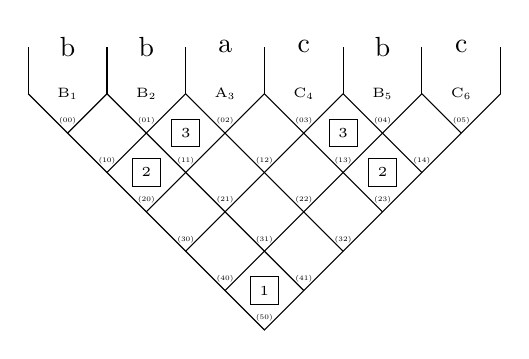
\begin{tikzpicture}[baseline]
			\newcommand{\myfontvars}[1]{
				\fontsize{4.9}{12}\selectfont{#1}
			}\newcommand{\myfontnumbering}[1]{
				\fontsize{2.5}{12}\selectfont{#1}
			}%Outer hull
			%Tip of the pyramid
			\coordinate (tip) at (3.0,-3.0);
			\foreach \i in {0,...,6} {
				\coordinate (\i) at (\i,0);
			}
			%Draw the left and right line of the pyramid pointing downwards
			\draw (0) -- (tip) -- (6);
			%Grid lines direction down-left to top-right
			\coordinate (dl1) at (0.5,-0.5);
			\coordinate (dl2) at (1.0,-1.0);
			\coordinate (dl3) at (1.5,-1.5);
			\coordinate (dl4) at (2.0,-2.0);
			\coordinate (dl5) at (2.5,-2.5);
			\draw (dl1) -- (1,0);
			\draw (dl2) -- (2,0);
			\draw (dl3) -- (3,0);
			\draw (dl4) -- (4,0);
			\draw (dl5) -- (5,0);
			%Grid lines direction down-right to top-left
			\coordinate (dr1) at (3.5,-2.5);
			\coordinate (dr2) at (4.0,-2.0);
			\coordinate (dr3) at (4.5,-1.5);
			\coordinate (dr4) at (5.0,-1.0);
			\coordinate (dr5) at (5.5,-0.5);
			\draw (dr1) -- (1,0);
			\draw (dr2) -- (2,0);
			\draw (dr3) -- (3,0);
			\draw (dr4) -- (4,0);
			\draw (dr5) -- (5,0);
			%Small lines at the top
			\coordinate (top0) at (0.0,0.0);
			\coordinate (top1) at (1.0,0.0);
			\coordinate (top2) at (2.0,0.0);
			\coordinate (top3) at (3.0,0.0);
			\coordinate (top4) at (4.0,0.0);
			\coordinate (top5) at (5.0,0.0);
			\coordinate (top6) at (6.0,0.0);
			\coordinate (topUpper0) at (0.0,0.6);
			\coordinate (topUpper1) at (1.0,0.6);
			\coordinate (topUpper2) at (2.0,0.6);
			\coordinate (topUpper3) at (3.0,0.6);
			\coordinate (topUpper4) at (4.0,0.6);
			\coordinate (topUpper5) at (5.0,0.6);
			\coordinate (topUpper6) at (6.0,0.6);
			\draw (top0) -- (topUpper0);
			\draw (top1) -- (topUpper1);
			\draw (top2) -- (topUpper2);
			\draw (top3) -- (topUpper3);
			\draw (top4) -- (topUpper4);
			\draw (top5) -- (topUpper5);
			\draw (top6) -- (topUpper6);
			%The string
			\coordinate (w0) at (0.5,0.6);
			\coordinate (w1) at (1.5,0.6);
			\coordinate (w2) at (2.5,0.6);
			\coordinate (w3) at (3.5,0.6);
			\coordinate (w4) at (4.5,0.6);
			\coordinate (w5) at (5.5,0.6);
			\node [] at (w0) {b};
			\node [] at (w1) {b};
			\node [] at (w2) {a};
			\node [] at (w3) {c};
			\node [] at (w4) {b};
			\node [] at (w5) {c};
			% Variables in the cells
			%cells00
			\coordinate (center00) at (0.5,0.0);
			\node [below=0.18cm] at (center00) {\myfontnumbering{$(00)$}};
			\node [] at (center00) {\myfontvars{B$_{1}$}};
			%cells01
			\coordinate (center01) at (1.5,0.0);
			\node [below=0.18cm] at (center01) {\myfontnumbering{$(01)$}};
			\node [] at (center01) {\myfontvars{B$_{2}$}};
			%cells02
			\coordinate (center02) at (2.5,0.0);
			\node [below=0.18cm] at (center02) {\myfontnumbering{$(02)$}};
			\node [] at (center02) {\myfontvars{A$_{3}$}};
			%cells03
			\coordinate (center03) at (3.5,0.0);
			\node [below=0.18cm] at (center03) {\myfontnumbering{$(03)$}};
			\node [] at (center03) {\myfontvars{C$_{4}$}};
			%cells04
			\coordinate (center04) at (4.5,0.0);
			\node [below=0.18cm] at (center04) {\myfontnumbering{$(04)$}};
			\node [] at (center04) {\myfontvars{B$_{5}$}};
			%cells05
			\coordinate (center05) at (5.5,0.0);
			\node [below=0.18cm] at (center05) {\myfontnumbering{$(05)$}};
			\node [] at (center05) {\myfontvars{C$_{6}$}};
			%cells10
			\coordinate (center10) at (1.0,-0.5);
			\node [below=0.18cm] at (center10) {\myfontnumbering{$(10)$}};
			%cells11
			\coordinate (center11) at (2.0,-0.5);
			\node [below=0.18cm] at (center11) {\myfontnumbering{$(11)$}};
			\node [] at (center11) [minimum height=0.25cm,minimum width=0.25cm,draw] {\tiny{3}};
			%cells12
			\coordinate (center12) at (3.0,-0.5);
			\node [below=0.18cm] at (center12) {\myfontnumbering{$(12)$}};
			%cells13
			\coordinate (center13) at (4.0,-0.5);
			\node [below=0.18cm] at (center13) {\myfontnumbering{$(13)$}};
			\node [] at (center13) [minimum height=0.25cm,minimum width=0.25cm,draw] {\tiny{3}};
			%cells14
			\coordinate (center14) at (5.0,-0.5);
			\node [below=0.18cm] at (center14) {\myfontnumbering{$(14)$}};
			%cells20
			\coordinate (center20) at (1.5,-1.0);
			\node [below=0.18cm] at (center20) {\myfontnumbering{$(20)$}};
			\node [] at (center20) [minimum height=0.25cm,minimum width=0.25cm,draw] {\tiny{2}};
			%cells21
			\coordinate (center21) at (2.5,-1.0);
			\node [below=0.18cm] at (center21) {\myfontnumbering{$(21)$}};
			%cells22
			\coordinate (center22) at (3.5,-1.0);
			\node [below=0.18cm] at (center22) {\myfontnumbering{$(22)$}};
			%cells23
			\coordinate (center23) at (4.5,-1.0);
			\node [below=0.18cm] at (center23) {\myfontnumbering{$(23)$}};
			\node [] at (center23) [minimum height=0.25cm,minimum width=0.25cm,draw] {\tiny{2}};
			%cells30
			\coordinate (center30) at (2.0,-1.5);
			\node [below=0.18cm] at (center30) {\myfontnumbering{$(30)$}};
			%cells31
			\coordinate (center31) at (3.0,-1.5);
			\node [below=0.18cm] at (center31) {\myfontnumbering{$(31)$}};
			%cells32
			\coordinate (center32) at (4.0,-1.5);
			\node [below=0.18cm] at (center32) {\myfontnumbering{$(32)$}};
			%cells40
			\coordinate (center40) at (2.5,-2.0);
			\node [below=0.18cm] at (center40) {\myfontnumbering{$(40)$}};
			%cells41
			\coordinate (center41) at (3.5,-2.0);
			\node [below=0.18cm] at (center41) {\myfontnumbering{$(41)$}};
			%cells50
			\coordinate (center50) at (3.0,-2.5);
			\node [below=0.18cm] at (center50) {\myfontnumbering{$(50)$}};
			\node [] at (center50) [minimum height=0.25cm,minimum width=0.25cm,draw] {\tiny{1}};
			\end{tikzpicture}
		}
	\end{minipage}
	\captionof{figure}{Illustration of Algorithm \ref{SplitThenFill} SplitThenFill part 1 after adding $A \rightarrow a$, $B \rightarrow b$ and $C \rightarrow c$.}
	\label{IllustrationAlgorithmSplitThenFillPart1}
	~
	
	\noindent After adding the terminals to the grammar now the recursion step at $Cell_{1,1}$ is taken on. Now $Cell_l=\{B_2\}$ and $Cell_r=\{A_3\}$ and therefore $VarComp=\{BA\}$. Adding the rule $S \rightarrow BA$ leads to the following $Pyramid$ shown in Figure \ref{IllustrationAlgorithmSplitThenFillPart2}: \\
	
	\begin{minipage}{6in}
			\centering
			\begin{tabular}{l}
				Grammar:\\
				$A \rightarrow a$\\
				$B \rightarrow b$\\ 
				$C \rightarrow c$\\
				$S \rightarrow \textbf{BA}$\\ 
			\end{tabular} 
			\resizebox{0.7\linewidth}{!}{
				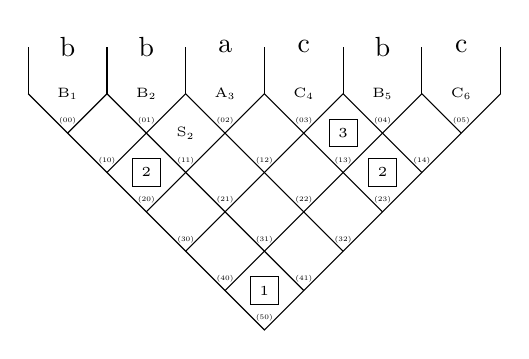
\begin{tikzpicture}[baseline]
				\newcommand{\myfontvars}[1]{
					\fontsize{4.9}{12}\selectfont{#1}
				}\newcommand{\myfontnumbering}[1]{
					\fontsize{2.5}{12}\selectfont{#1}
				}%Outer hull
				%Tip of the pyramid
				\coordinate (tip) at (3.0,-3.0);
				\foreach \i in {0,...,6} {
					\coordinate (\i) at (\i,0);
				}
				%Draw the left and right line of the pyramid pointing downwards
				\draw (0) -- (tip) -- (6);
				%Grid lines direction down-left to top-right
				\coordinate (dl1) at (0.5,-0.5);
				\coordinate (dl2) at (1.0,-1.0);
				\coordinate (dl3) at (1.5,-1.5);
				\coordinate (dl4) at (2.0,-2.0);
				\coordinate (dl5) at (2.5,-2.5);
				\draw (dl1) -- (1,0);
				\draw (dl2) -- (2,0);
				\draw (dl3) -- (3,0);
				\draw (dl4) -- (4,0);
				\draw (dl5) -- (5,0);
				%Grid lines direction down-right to top-left
				\coordinate (dr1) at (3.5,-2.5);
				\coordinate (dr2) at (4.0,-2.0);
				\coordinate (dr3) at (4.5,-1.5);
				\coordinate (dr4) at (5.0,-1.0);
				\coordinate (dr5) at (5.5,-0.5);
				\draw (dr1) -- (1,0);
				\draw (dr2) -- (2,0);
				\draw (dr3) -- (3,0);
				\draw (dr4) -- (4,0);
				\draw (dr5) -- (5,0);
				%Small lines at the top
				\coordinate (top0) at (0.0,0.0);
				\coordinate (top1) at (1.0,0.0);
				\coordinate (top2) at (2.0,0.0);
				\coordinate (top3) at (3.0,0.0);
				\coordinate (top4) at (4.0,0.0);
				\coordinate (top5) at (5.0,0.0);
				\coordinate (top6) at (6.0,0.0);
				\coordinate (topUpper0) at (0.0,0.6);
				\coordinate (topUpper1) at (1.0,0.6);
				\coordinate (topUpper2) at (2.0,0.6);
				\coordinate (topUpper3) at (3.0,0.6);
				\coordinate (topUpper4) at (4.0,0.6);
				\coordinate (topUpper5) at (5.0,0.6);
				\coordinate (topUpper6) at (6.0,0.6);
				\draw (top0) -- (topUpper0);
				\draw (top1) -- (topUpper1);
				\draw (top2) -- (topUpper2);
				\draw (top3) -- (topUpper3);
				\draw (top4) -- (topUpper4);
				\draw (top5) -- (topUpper5);
				\draw (top6) -- (topUpper6);
				%The string
				\coordinate (w0) at (0.5,0.6);
				\coordinate (w1) at (1.5,0.6);
				\coordinate (w2) at (2.5,0.6);
				\coordinate (w3) at (3.5,0.6);
				\coordinate (w4) at (4.5,0.6);
				\coordinate (w5) at (5.5,0.6);
				\node [] at (w0) {b};
				\node [] at (w1) {b};
				\node [] at (w2) {a};
				\node [] at (w3) {c};
				\node [] at (w4) {b};
				\node [] at (w5) {c};
				% Variables in the cells
				%cells00
				\coordinate (center00) at (0.5,0.0);
				\node [below=0.18cm] at (center00) {\myfontnumbering{$(00)$}};
				\node [] at (center00) {\myfontvars{B$_{1}$}};
				%cells01
				\coordinate (center01) at (1.5,0.0);
				\node [below=0.18cm] at (center01) {\myfontnumbering{$(01)$}};
				\node [] at (center01) {\myfontvars{B$_{2}$}};
				%cells02
				\coordinate (center02) at (2.5,0.0);
				\node [below=0.18cm] at (center02) {\myfontnumbering{$(02)$}};
				\node [] at (center02) {\myfontvars{A$_{3}$}};
				%cells03
				\coordinate (center03) at (3.5,0.0);
				\node [below=0.18cm] at (center03) {\myfontnumbering{$(03)$}};
				\node [] at (center03) {\myfontvars{C$_{4}$}};
				%cells04
				\coordinate (center04) at (4.5,0.0);
				\node [below=0.18cm] at (center04) {\myfontnumbering{$(04)$}};
				\node [] at (center04) {\myfontvars{B$_{5}$}};
				%cells05
				\coordinate (center05) at (5.5,0.0);
				\node [below=0.18cm] at (center05) {\myfontnumbering{$(05)$}};
				\node [] at (center05) {\myfontvars{C$_{6}$}};
				%cells10
				\coordinate (center10) at (1.0,-0.5);
				\node [below=0.18cm] at (center10) {\myfontnumbering{$(10)$}};
				%cells11
				\coordinate (center11) at (2.0,-0.5);
				\node [below=0.18cm] at (center11) {\myfontnumbering{$(11)$}};
				\node [] at (center11) {\myfontvars{S$_{2}$}};
				%cells12
				\coordinate (center12) at (3.0,-0.5);
				\node [below=0.18cm] at (center12) {\myfontnumbering{$(12)$}};
				%cells13
				\coordinate (center13) at (4.0,-0.5);
				\node [below=0.18cm] at (center13) {\myfontnumbering{$(13)$}};
				\node [] at (center13) [minimum height=0.25cm,minimum width=0.25cm,draw] {\tiny{3}};
				%cells14
				\coordinate (center14) at (5.0,-0.5);
				\node [below=0.18cm] at (center14) {\myfontnumbering{$(14)$}};
				%cells20
				\coordinate (center20) at (1.5,-1.0);
				\node [below=0.18cm] at (center20) {\myfontnumbering{$(20)$}};
				\node [] at (center20) [minimum height=0.25cm,minimum width=0.25cm,draw] {\tiny{2}};
				%cells21
				\coordinate (center21) at (2.5,-1.0);
				\node [below=0.18cm] at (center21) {\myfontnumbering{$(21)$}};
				%cells22
				\coordinate (center22) at (3.5,-1.0);
				\node [below=0.18cm] at (center22) {\myfontnumbering{$(22)$}};
				%cells23
				\coordinate (center23) at (4.5,-1.0);
				\node [below=0.18cm] at (center23) {\myfontnumbering{$(23)$}};
				\node [] at (center23) [minimum height=0.25cm,minimum width=0.25cm,draw] {\tiny{2}};
				%cells30
				\coordinate (center30) at (2.0,-1.5);
				\node [below=0.18cm] at (center30) {\myfontnumbering{$(30)$}};
				%cells31
				\coordinate (center31) at (3.0,-1.5);
				\node [below=0.18cm] at (center31) {\myfontnumbering{$(31)$}};
				%cells32
				\coordinate (center32) at (4.0,-1.5);
				\node [below=0.18cm] at (center32) {\myfontnumbering{$(32)$}};
				%cells40
				\coordinate (center40) at (2.5,-2.0);
				\node [below=0.18cm] at (center40) {\myfontnumbering{$(40)$}};
				%cells41
				\coordinate (center41) at (3.5,-2.0);
				\node [below=0.18cm] at (center41) {\myfontnumbering{$(41)$}};
				%cells50
				\coordinate (center50) at (3.0,-2.5);
				\node [below=0.18cm] at (center50) {\myfontnumbering{$(50)$}};
				\node [] at (center50) [minimum height=0.25cm,minimum width=0.25cm,draw] {\tiny{1}};
				\end{tikzpicture}
			}
		\end{minipage}
		\captionof{figure}{Illustration of Algorithm \ref{SplitThenFill} SplitThenFill part 2 after adding $S\rightarrow BA$.}
		\label{IllustrationAlgorithmSplitThenFillPart2}
		
		\noindent The next recursion step happens in $Cell_{2,0}$. Now $Cell_l=\{B_1\}$ and $Cell_r=\{S_2\}$. Analogously the rule $A\rightarrow BS$ is added to the grammar as seen in Figure \ref{IllustrationAlgorithmSplitThenFillPart3}:\\
		
		\begin{minipage}{6in}
			\centering
			\begin{tabular}{l}
				Grammar:\\
				$A \rightarrow \textbf{BS}~|~a$\\
				$B \rightarrow b$\\ 
				$C \rightarrow c$\\
				$S \rightarrow BA$\\ 
			\end{tabular} 
			\resizebox{0.7\linewidth}{!}{
				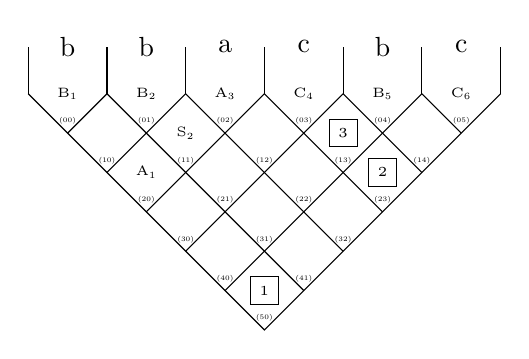
\begin{tikzpicture}[baseline]
				\newcommand{\myfontvars}[1]{
					\fontsize{4.9}{12}\selectfont{#1}
				}\newcommand{\myfontnumbering}[1]{
					\fontsize{2.5}{12}\selectfont{#1}
				}%Outer hull
				%Tip of the pyramid
				\coordinate (tip) at (3.0,-3.0);
				\foreach \i in {0,...,6} {
					\coordinate (\i) at (\i,0);
				}
				%Draw the left and right line of the pyramid pointing downwards
				\draw (0) -- (tip) -- (6);
				%Grid lines direction down-left to top-right
				\coordinate (dl1) at (0.5,-0.5);
				\coordinate (dl2) at (1.0,-1.0);
				\coordinate (dl3) at (1.5,-1.5);
				\coordinate (dl4) at (2.0,-2.0);
				\coordinate (dl5) at (2.5,-2.5);
				\draw (dl1) -- (1,0);
				\draw (dl2) -- (2,0);
				\draw (dl3) -- (3,0);
				\draw (dl4) -- (4,0);
				\draw (dl5) -- (5,0);
				%Grid lines direction down-right to top-left
				\coordinate (dr1) at (3.5,-2.5);
				\coordinate (dr2) at (4.0,-2.0);
				\coordinate (dr3) at (4.5,-1.5);
				\coordinate (dr4) at (5.0,-1.0);
				\coordinate (dr5) at (5.5,-0.5);
				\draw (dr1) -- (1,0);
				\draw (dr2) -- (2,0);
				\draw (dr3) -- (3,0);
				\draw (dr4) -- (4,0);
				\draw (dr5) -- (5,0);
				%Small lines at the top
				\coordinate (top0) at (0.0,0.0);
				\coordinate (top1) at (1.0,0.0);
				\coordinate (top2) at (2.0,0.0);
				\coordinate (top3) at (3.0,0.0);
				\coordinate (top4) at (4.0,0.0);
				\coordinate (top5) at (5.0,0.0);
				\coordinate (top6) at (6.0,0.0);
				\coordinate (topUpper0) at (0.0,0.6);
				\coordinate (topUpper1) at (1.0,0.6);
				\coordinate (topUpper2) at (2.0,0.6);
				\coordinate (topUpper3) at (3.0,0.6);
				\coordinate (topUpper4) at (4.0,0.6);
				\coordinate (topUpper5) at (5.0,0.6);
				\coordinate (topUpper6) at (6.0,0.6);
				\draw (top0) -- (topUpper0);
				\draw (top1) -- (topUpper1);
				\draw (top2) -- (topUpper2);
				\draw (top3) -- (topUpper3);
				\draw (top4) -- (topUpper4);
				\draw (top5) -- (topUpper5);
				\draw (top6) -- (topUpper6);
				%The string
				\coordinate (w0) at (0.5,0.6);
				\coordinate (w1) at (1.5,0.6);
				\coordinate (w2) at (2.5,0.6);
				\coordinate (w3) at (3.5,0.6);
				\coordinate (w4) at (4.5,0.6);
				\coordinate (w5) at (5.5,0.6);
				\node [] at (w0) {b};
				\node [] at (w1) {b};
				\node [] at (w2) {a};
				\node [] at (w3) {c};
				\node [] at (w4) {b};
				\node [] at (w5) {c};
				% Variables in the cells
				%cells00
				\coordinate (center00) at (0.5,0.0);
				\node [below=0.18cm] at (center00) {\myfontnumbering{$(00)$}};
				\node [] at (center00) {\myfontvars{B$_{1}$}};
				%cells01
				\coordinate (center01) at (1.5,0.0);
				\node [below=0.18cm] at (center01) {\myfontnumbering{$(01)$}};
				\node [] at (center01) {\myfontvars{B$_{2}$}};
				%cells02
				\coordinate (center02) at (2.5,0.0);
				\node [below=0.18cm] at (center02) {\myfontnumbering{$(02)$}};
				\node [] at (center02) {\myfontvars{A$_{3}$}};
				%cells03
				\coordinate (center03) at (3.5,0.0);
				\node [below=0.18cm] at (center03) {\myfontnumbering{$(03)$}};
				\node [] at (center03) {\myfontvars{C$_{4}$}};
				%cells04
				\coordinate (center04) at (4.5,0.0);
				\node [below=0.18cm] at (center04) {\myfontnumbering{$(04)$}};
				\node [] at (center04) {\myfontvars{B$_{5}$}};
				%cells05
				\coordinate (center05) at (5.5,0.0);
				\node [below=0.18cm] at (center05) {\myfontnumbering{$(05)$}};
				\node [] at (center05) {\myfontvars{C$_{6}$}};
				%cells10
				\coordinate (center10) at (1.0,-0.5);
				\node [below=0.18cm] at (center10) {\myfontnumbering{$(10)$}};
				%cells11
				\coordinate (center11) at (2.0,-0.5);
				\node [below=0.18cm] at (center11) {\myfontnumbering{$(11)$}};
				\node [] at (center11) {\myfontvars{S$_{2}$}};
				%cells12
				\coordinate (center12) at (3.0,-0.5);
				\node [below=0.18cm] at (center12) {\myfontnumbering{$(12)$}};
				%cells13
				\coordinate (center13) at (4.0,-0.5);
				\node [below=0.18cm] at (center13) {\myfontnumbering{$(13)$}};
				\node [] at (center13) [minimum height=0.25cm,minimum width=0.25cm,draw] {\tiny{3}};
				%cells14
				\coordinate (center14) at (5.0,-0.5);
				\node [below=0.18cm] at (center14) {\myfontnumbering{$(14)$}};
				%cells20
				\coordinate (center20) at (1.5,-1.0);
				\node [below=0.18cm] at (center20) {\myfontnumbering{$(20)$}};
				\node [] at (center20) {\myfontvars{A$_{1}$}};
				%cells21
				\coordinate (center21) at (2.5,-1.0);
				\node [below=0.18cm] at (center21) {\myfontnumbering{$(21)$}};
				%cells22
				\coordinate (center22) at (3.5,-1.0);
				\node [below=0.18cm] at (center22) {\myfontnumbering{$(22)$}};
				%cells23
				\coordinate (center23) at (4.5,-1.0);
				\node [below=0.18cm] at (center23) {\myfontnumbering{$(23)$}};
				\node [] at (center23) [minimum height=0.25cm,minimum width=0.25cm,draw] {\tiny{2}};
				%cells30
				\coordinate (center30) at (2.0,-1.5);
				\node [below=0.18cm] at (center30) {\myfontnumbering{$(30)$}};
				%cells31
				\coordinate (center31) at (3.0,-1.5);
				\node [below=0.18cm] at (center31) {\myfontnumbering{$(31)$}};
				%cells32
				\coordinate (center32) at (4.0,-1.5);
				\node [below=0.18cm] at (center32) {\myfontnumbering{$(32)$}};
				%cells40
				\coordinate (center40) at (2.5,-2.0);
				\node [below=0.18cm] at (center40) {\myfontnumbering{$(40)$}};
				%cells41
				\coordinate (center41) at (3.5,-2.0);
				\node [below=0.18cm] at (center41) {\myfontnumbering{$(41)$}};
				%cells50
				\coordinate (center50) at (3.0,-2.5);
				\node [below=0.18cm] at (center50) {\myfontnumbering{$(50)$}};
				\node [] at (center50) [minimum height=0.25cm,minimum width=0.25cm,draw] {\tiny{1}};
				\end{tikzpicture}
			}
		\end{minipage}
		\captionof{figure}{Illustration of Algorithm \ref{SplitThenFill} SplitThenFill part 3 after adding the rule $A\rightarrow BS$.}
		\label{IllustrationAlgorithmSplitThenFillPart3}
		~\\
		The next two analogous steps are described with Figure \ref{IllustrationAlgorithmSplitThenFillPart4} and with Figure \ref{IllustrationAlgorithmSplitThenFillPart5}. \\
		
		\begin{minipage}{6in}
			\centering
			\centering
			\begin{tabular}{l}
				Grammar:\\
				$A \rightarrow BS~|~a$\\
				$B \rightarrow \textbf{CB}~|~b$\\ 
				$C \rightarrow c$\\
				$S \rightarrow BA$\\ 
			\end{tabular} 
			\resizebox{0.7\linewidth}{!}{
				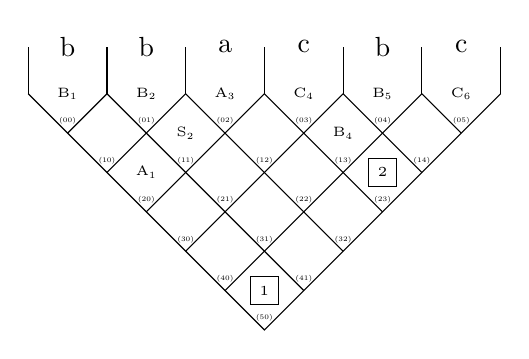
\begin{tikzpicture}[baseline]
				\newcommand{\myfontvars}[1]{
					\fontsize{4.9}{12}\selectfont{#1}
				}\newcommand{\myfontnumbering}[1]{
					\fontsize{2.5}{12}\selectfont{#1}
				}%Outer hull
				%Tip of the pyramid
				\coordinate (tip) at (3.0,-3.0);
				\foreach \i in {0,...,6} {
					\coordinate (\i) at (\i,0);
				}
				%Draw the left and right line of the pyramid pointing downwards
				\draw (0) -- (tip) -- (6);
				%Grid lines direction down-left to top-right
				\coordinate (dl1) at (0.5,-0.5);
				\coordinate (dl2) at (1.0,-1.0);
				\coordinate (dl3) at (1.5,-1.5);
				\coordinate (dl4) at (2.0,-2.0);
				\coordinate (dl5) at (2.5,-2.5);
				\draw (dl1) -- (1,0);
				\draw (dl2) -- (2,0);
				\draw (dl3) -- (3,0);
				\draw (dl4) -- (4,0);
				\draw (dl5) -- (5,0);
				%Grid lines direction down-right to top-left
				\coordinate (dr1) at (3.5,-2.5);
				\coordinate (dr2) at (4.0,-2.0);
				\coordinate (dr3) at (4.5,-1.5);
				\coordinate (dr4) at (5.0,-1.0);
				\coordinate (dr5) at (5.5,-0.5);
				\draw (dr1) -- (1,0);
				\draw (dr2) -- (2,0);
				\draw (dr3) -- (3,0);
				\draw (dr4) -- (4,0);
				\draw (dr5) -- (5,0);
				%Small lines at the top
				\coordinate (top0) at (0.0,0.0);
				\coordinate (top1) at (1.0,0.0);
				\coordinate (top2) at (2.0,0.0);
				\coordinate (top3) at (3.0,0.0);
				\coordinate (top4) at (4.0,0.0);
				\coordinate (top5) at (5.0,0.0);
				\coordinate (top6) at (6.0,0.0);
				\coordinate (topUpper0) at (0.0,0.6);
				\coordinate (topUpper1) at (1.0,0.6);
				\coordinate (topUpper2) at (2.0,0.6);
				\coordinate (topUpper3) at (3.0,0.6);
				\coordinate (topUpper4) at (4.0,0.6);
				\coordinate (topUpper5) at (5.0,0.6);
				\coordinate (topUpper6) at (6.0,0.6);
				\draw (top0) -- (topUpper0);
				\draw (top1) -- (topUpper1);
				\draw (top2) -- (topUpper2);
				\draw (top3) -- (topUpper3);
				\draw (top4) -- (topUpper4);
				\draw (top5) -- (topUpper5);
				\draw (top6) -- (topUpper6);
				%The string
				\coordinate (w0) at (0.5,0.6);
				\coordinate (w1) at (1.5,0.6);
				\coordinate (w2) at (2.5,0.6);
				\coordinate (w3) at (3.5,0.6);
				\coordinate (w4) at (4.5,0.6);
				\coordinate (w5) at (5.5,0.6);
				\node [] at (w0) {b};
				\node [] at (w1) {b};
				\node [] at (w2) {a};
				\node [] at (w3) {c};
				\node [] at (w4) {b};
				\node [] at (w5) {c};
				% Variables in the cells
				%cells00
				\coordinate (center00) at (0.5,0.0);
				\node [below=0.18cm] at (center00) {\myfontnumbering{$(00)$}};
				\node [] at (center00) {\myfontvars{B$_{1}$}};
				%cells01
				\coordinate (center01) at (1.5,0.0);
				\node [below=0.18cm] at (center01) {\myfontnumbering{$(01)$}};
				\node [] at (center01) {\myfontvars{B$_{2}$}};
				%cells02
				\coordinate (center02) at (2.5,0.0);
				\node [below=0.18cm] at (center02) {\myfontnumbering{$(02)$}};
				\node [] at (center02) {\myfontvars{A$_{3}$}};
				%cells03
				\coordinate (center03) at (3.5,0.0);
				\node [below=0.18cm] at (center03) {\myfontnumbering{$(03)$}};
				\node [] at (center03) {\myfontvars{C$_{4}$}};
				%cells04
				\coordinate (center04) at (4.5,0.0);
				\node [below=0.18cm] at (center04) {\myfontnumbering{$(04)$}};
				\node [] at (center04) {\myfontvars{B$_{5}$}};
				%cells05
				\coordinate (center05) at (5.5,0.0);
				\node [below=0.18cm] at (center05) {\myfontnumbering{$(05)$}};
				\node [] at (center05) {\myfontvars{C$_{6}$}};
				%cells10
				\coordinate (center10) at (1.0,-0.5);
				\node [below=0.18cm] at (center10) {\myfontnumbering{$(10)$}};
				%cells11
				\coordinate (center11) at (2.0,-0.5);
				\node [below=0.18cm] at (center11) {\myfontnumbering{$(11)$}};
				\node [] at (center11) {\myfontvars{S$_{2}$}};
				%cells12
				\coordinate (center12) at (3.0,-0.5);
				\node [below=0.18cm] at (center12) {\myfontnumbering{$(12)$}};
				%cells13
				\coordinate (center13) at (4.0,-0.5);
				\node [below=0.18cm] at (center13) {\myfontnumbering{$(13)$}};
				\node [] at (center13) {\myfontvars{B$_{4}$}};
				%cells14
				\coordinate (center14) at (5.0,-0.5);
				\node [below=0.18cm] at (center14) {\myfontnumbering{$(14)$}};
				%cells20
				\coordinate (center20) at (1.5,-1.0);
				\node [below=0.18cm] at (center20) {\myfontnumbering{$(20)$}};
				\node [] at (center20) {\myfontvars{A$_{1}$}};
				%cells21
				\coordinate (center21) at (2.5,-1.0);
				\node [below=0.18cm] at (center21) {\myfontnumbering{$(21)$}};
				%cells22
				\coordinate (center22) at (3.5,-1.0);
				\node [below=0.18cm] at (center22) {\myfontnumbering{$(22)$}};
				%cells23
				\coordinate (center23) at (4.5,-1.0);
				\node [below=0.18cm] at (center23) {\myfontnumbering{$(23)$}};
				\node [] at (center23) [minimum height=0.25cm,minimum width=0.25cm,draw] {\tiny{2}};
				%cells30
				\coordinate (center30) at (2.0,-1.5);
				\node [below=0.18cm] at (center30) {\myfontnumbering{$(30)$}};
				%cells31
				\coordinate (center31) at (3.0,-1.5);
				\node [below=0.18cm] at (center31) {\myfontnumbering{$(31)$}};
				%cells32
				\coordinate (center32) at (4.0,-1.5);
				\node [below=0.18cm] at (center32) {\myfontnumbering{$(32)$}};
				%cells40
				\coordinate (center40) at (2.5,-2.0);
				\node [below=0.18cm] at (center40) {\myfontnumbering{$(40)$}};
				%cells41
				\coordinate (center41) at (3.5,-2.0);
				\node [below=0.18cm] at (center41) {\myfontnumbering{$(41)$}};
				%cells50
				\coordinate (center50) at (3.0,-2.5);
				\node [below=0.18cm] at (center50) {\myfontnumbering{$(50)$}};
				\node [] at (center50) [minimum height=0.25cm,minimum width=0.25cm,draw] {\tiny{1}};
				\end{tikzpicture}
			}
		\end{minipage}
		\captionof{figure}{Illustration of Algorithm \ref{SplitThenFill} SplitThenFill part 4. The recursion step in $Cell_{1,3}$ is  resolved by adding the rule $B\rightarrow CB$.}
		\label{IllustrationAlgorithmSplitThenFillPart4}
		\pagebreak \clearpage
		
		\begin{minipage}{6in}
			\centering
			\begin{tabular}{l}
				Grammar:\\
				$A \rightarrow BS~|~a$\\
				$B \rightarrow CB~|~b$\\ 
				$C \rightarrow \textbf{BC}~|~c$\\
				$S \rightarrow BA$\\ 
			\end{tabular} 
			\resizebox{0.7\linewidth}{!}{
				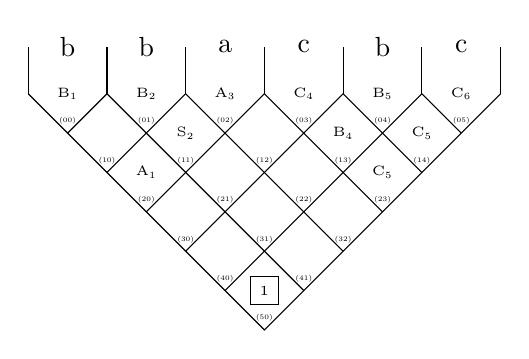
\begin{tikzpicture}[baseline]
				\newcommand{\myfontvars}[1]{
					\fontsize{4.9}{12}\selectfont{#1}
				}\newcommand{\myfontnumbering}[1]{
					\fontsize{2.5}{12}\selectfont{#1}
				}%Outer hull
				%Tip of the pyramid
				\coordinate (tip) at (3.0,-3.0);
				\foreach \i in {0,...,6} {
					\coordinate (\i) at (\i,0);
				}
				%Draw the left and right line of the pyramid pointing downwards
				\draw (0) -- (tip) -- (6);
				%Grid lines direction down-left to top-right
				\coordinate (dl1) at (0.5,-0.5);
				\coordinate (dl2) at (1.0,-1.0);
				\coordinate (dl3) at (1.5,-1.5);
				\coordinate (dl4) at (2.0,-2.0);
				\coordinate (dl5) at (2.5,-2.5);
				\draw (dl1) -- (1,0);
				\draw (dl2) -- (2,0);
				\draw (dl3) -- (3,0);
				\draw (dl4) -- (4,0);
				\draw (dl5) -- (5,0);
				%Grid lines direction down-right to top-left
				\coordinate (dr1) at (3.5,-2.5);
				\coordinate (dr2) at (4.0,-2.0);
				\coordinate (dr3) at (4.5,-1.5);
				\coordinate (dr4) at (5.0,-1.0);
				\coordinate (dr5) at (5.5,-0.5);
				\draw (dr1) -- (1,0);
				\draw (dr2) -- (2,0);
				\draw (dr3) -- (3,0);
				\draw (dr4) -- (4,0);
				\draw (dr5) -- (5,0);
				%Small lines at the top
				\coordinate (top0) at (0.0,0.0);
				\coordinate (top1) at (1.0,0.0);
				\coordinate (top2) at (2.0,0.0);
				\coordinate (top3) at (3.0,0.0);
				\coordinate (top4) at (4.0,0.0);
				\coordinate (top5) at (5.0,0.0);
				\coordinate (top6) at (6.0,0.0);
				\coordinate (topUpper0) at (0.0,0.6);
				\coordinate (topUpper1) at (1.0,0.6);
				\coordinate (topUpper2) at (2.0,0.6);
				\coordinate (topUpper3) at (3.0,0.6);
				\coordinate (topUpper4) at (4.0,0.6);
				\coordinate (topUpper5) at (5.0,0.6);
				\coordinate (topUpper6) at (6.0,0.6);
				\draw (top0) -- (topUpper0);
				\draw (top1) -- (topUpper1);
				\draw (top2) -- (topUpper2);
				\draw (top3) -- (topUpper3);
				\draw (top4) -- (topUpper4);
				\draw (top5) -- (topUpper5);
				\draw (top6) -- (topUpper6);
				%The string
				\coordinate (w0) at (0.5,0.6);
				\coordinate (w1) at (1.5,0.6);
				\coordinate (w2) at (2.5,0.6);
				\coordinate (w3) at (3.5,0.6);
				\coordinate (w4) at (4.5,0.6);
				\coordinate (w5) at (5.5,0.6);
				\node [] at (w0) {b};
				\node [] at (w1) {b};
				\node [] at (w2) {a};
				\node [] at (w3) {c};
				\node [] at (w4) {b};
				\node [] at (w5) {c};
				% Variables in the cells
				%cells00
				\coordinate (center00) at (0.5,0.0);
				\node [below=0.18cm] at (center00) {\myfontnumbering{$(00)$}};
				\node [] at (center00) {\myfontvars{B$_{1}$}};
				%cells01
				\coordinate (center01) at (1.5,0.0);
				\node [below=0.18cm] at (center01) {\myfontnumbering{$(01)$}};
				\node [] at (center01) {\myfontvars{B$_{2}$}};
				%cells02
				\coordinate (center02) at (2.5,0.0);
				\node [below=0.18cm] at (center02) {\myfontnumbering{$(02)$}};
				\node [] at (center02) {\myfontvars{A$_{3}$}};
				%cells03
				\coordinate (center03) at (3.5,0.0);
				\node [below=0.18cm] at (center03) {\myfontnumbering{$(03)$}};
				\node [] at (center03) {\myfontvars{C$_{4}$}};
				%cells04
				\coordinate (center04) at (4.5,0.0);
				\node [below=0.18cm] at (center04) {\myfontnumbering{$(04)$}};
				\node [] at (center04) {\myfontvars{B$_{5}$}};
				%cells05
				\coordinate (center05) at (5.5,0.0);
				\node [below=0.18cm] at (center05) {\myfontnumbering{$(05)$}};
				\node [] at (center05) {\myfontvars{C$_{6}$}};
				%cells10
				\coordinate (center10) at (1.0,-0.5);
				\node [below=0.18cm] at (center10) {\myfontnumbering{$(10)$}};
				%cells11
				\coordinate (center11) at (2.0,-0.5);
				\node [below=0.18cm] at (center11) {\myfontnumbering{$(11)$}};
				\node [] at (center11) {\myfontvars{S$_{2}$}};
				%cells12
				\coordinate (center12) at (3.0,-0.5);
				\node [below=0.18cm] at (center12) {\myfontnumbering{$(12)$}};
				%cells13
				\coordinate (center13) at (4.0,-0.5);
				\node [below=0.18cm] at (center13) {\myfontnumbering{$(13)$}};
				\node [] at (center13) {\myfontvars{B$_{4}$}};
				%cells14
				\coordinate (center14) at (5.0,-0.5);
				\node [below=0.18cm] at (center14) {\myfontnumbering{$(14)$}};
				\node [] at (center14) {\myfontvars{C$_{5}$}};
				%cells20
				\coordinate (center20) at (1.5,-1.0);
				\node [below=0.18cm] at (center20) {\myfontnumbering{$(20)$}};
				\node [] at (center20) {\myfontvars{A$_{1}$}};
				%cells21
				\coordinate (center21) at (2.5,-1.0);
				\node [below=0.18cm] at (center21) {\myfontnumbering{$(21)$}};
				%cells22
				\coordinate (center22) at (3.5,-1.0);
				\node [below=0.18cm] at (center22) {\myfontnumbering{$(22)$}};
				%cells23
				\coordinate (center23) at (4.5,-1.0);
				\node [below=0.18cm] at (center23) {\myfontnumbering{$(23)$}};
				\node [] at (center23) {\myfontvars{C$_{5}$}};
				%cells30
				\coordinate (center30) at (2.0,-1.5);
				\node [below=0.18cm] at (center30) {\myfontnumbering{$(30)$}};
				%cells31
				\coordinate (center31) at (3.0,-1.5);
				\node [below=0.18cm] at (center31) {\myfontnumbering{$(31)$}};
				%cells32
				\coordinate (center32) at (4.0,-1.5);
				\node [below=0.18cm] at (center32) {\myfontnumbering{$(32)$}};
				%cells40
				\coordinate (center40) at (2.5,-2.0);
				\node [below=0.18cm] at (center40) {\myfontnumbering{$(40)$}};
				%cells41
				\coordinate (center41) at (3.5,-2.0);
				\node [below=0.18cm] at (center41) {\myfontnumbering{$(41)$}};
				%cells50
				\coordinate (center50) at (3.0,-2.5);
				\node [below=0.18cm] at (center50) {\myfontnumbering{$(50)$}};
				\node [] at (center50) [minimum height=0.25cm,minimum width=0.25cm,draw] {\tiny{1}};
				\end{tikzpicture}
			}
		\end{minipage}
		\captionof{figure}{Illustration of Algorithm \ref{SplitThenFill} SplitThenFill part 5. The recursion step in $Cell_{2,3}$ is  resolved by adding the rule $C\rightarrow BC$.}
		\label{IllustrationAlgorithmSplitThenFillPart5}
		~\\
		\noindent Finally the last recursion step that decides on the content of the root cell is shown in Figure \ref{IllustrationAlgorithmSplitThenFillPart6}. In this case the start variable is contained in the root of the pyramid.\\
		
		\begin{minipage}{6in}
			\centering
			\begin{tabular}{l}
				$Grammar:$\\
				$A\rightarrow B S~|~a~~$\\ 
				$B\rightarrow C B~|~b$\\ 
				$C\rightarrow B C~|~ c$\\ 
				$S\rightarrow B A~|~\textbf{AC}~~$\\ 
			\end{tabular}
			\resizebox{0.7\linewidth}{!}{
				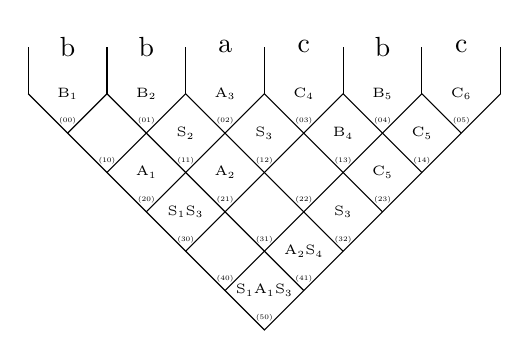
\begin{tikzpicture}[baseline]
				\newcommand{\myfontvars}[1]{
					\fontsize{4.9}{12}\selectfont{#1}
				}\newcommand{\myfontnumbering}[1]{
					\fontsize{2.5}{12}\selectfont{#1}
				}%Outer hull
				%Tip of the pyramid
				\coordinate (tip) at (3.0,-3.0);
				\foreach \i in {0,...,6} {
					\coordinate (\i) at (\i,0);
				}
				%Draw the left and right line of the pyramid pointing downwards
				\draw (0) -- (tip) -- (6);
				%Grid lines direction down-left to top-right
				\coordinate (dl1) at (0.5,-0.5);
				\coordinate (dl2) at (1.0,-1.0);
				\coordinate (dl3) at (1.5,-1.5);
				\coordinate (dl4) at (2.0,-2.0);
				\coordinate (dl5) at (2.5,-2.5);
				\draw (dl1) -- (1,0);
				\draw (dl2) -- (2,0);
				\draw (dl3) -- (3,0);
				\draw (dl4) -- (4,0);
				\draw (dl5) -- (5,0);
				%Grid lines direction down-right to top-left
				\coordinate (dr1) at (3.5,-2.5);
				\coordinate (dr2) at (4.0,-2.0);
				\coordinate (dr3) at (4.5,-1.5);
				\coordinate (dr4) at (5.0,-1.0);
				\coordinate (dr5) at (5.5,-0.5);
				\draw (dr1) -- (1,0);
				\draw (dr2) -- (2,0);
				\draw (dr3) -- (3,0);
				\draw (dr4) -- (4,0);
				\draw (dr5) -- (5,0);
				%Small lines at the top
				\coordinate (top0) at (0.0,0.0);
				\coordinate (top1) at (1.0,0.0);
				\coordinate (top2) at (2.0,0.0);
				\coordinate (top3) at (3.0,0.0);
				\coordinate (top4) at (4.0,0.0);
				\coordinate (top5) at (5.0,0.0);
				\coordinate (top6) at (6.0,0.0);
				\coordinate (topUpper0) at (0.0,0.6);
				\coordinate (topUpper1) at (1.0,0.6);
				\coordinate (topUpper2) at (2.0,0.6);
				\coordinate (topUpper3) at (3.0,0.6);
				\coordinate (topUpper4) at (4.0,0.6);
				\coordinate (topUpper5) at (5.0,0.6);
				\coordinate (topUpper6) at (6.0,0.6);
				\draw (top0) -- (topUpper0);
				\draw (top1) -- (topUpper1);
				\draw (top2) -- (topUpper2);
				\draw (top3) -- (topUpper3);
				\draw (top4) -- (topUpper4);
				\draw (top5) -- (topUpper5);
				\draw (top6) -- (topUpper6);
				%The string
				\coordinate (w0) at (0.5,0.6);
				\coordinate (w1) at (1.5,0.6);
				\coordinate (w2) at (2.5,0.6);
				\coordinate (w3) at (3.5,0.6);
				\coordinate (w4) at (4.5,0.6);
				\coordinate (w5) at (5.5,0.6);
				\node [] at (w0) {b};
				\node [] at (w1) {b};
				\node [] at (w2) {a};
				\node [] at (w3) {c};
				\node [] at (w4) {b};
				\node [] at (w5) {c};
				% Variables in the cells
				%cells00
				\coordinate (center00) at (0.5,0.0);
				\node [below=0.18cm] at (center00) {\myfontnumbering{$(00)$}};
				\node [] at (center00) {\myfontvars{B$_{1}$}};
				%cells01
				\coordinate (center01) at (1.5,0.0);
				\node [below=0.18cm] at (center01) {\myfontnumbering{$(01)$}};
				\node [] at (center01) {\myfontvars{B$_{2}$}};
				%cells02
				\coordinate (center02) at (2.5,0.0);
				\node [below=0.18cm] at (center02) {\myfontnumbering{$(02)$}};
				\node [] at (center02) {\myfontvars{A$_{3}$}};
				%cells03
				\coordinate (center03) at (3.5,0.0);
				\node [below=0.18cm] at (center03) {\myfontnumbering{$(03)$}};
				\node [] at (center03) {\myfontvars{C$_{4}$}};
				%cells04
				\coordinate (center04) at (4.5,0.0);
				\node [below=0.18cm] at (center04) {\myfontnumbering{$(04)$}};
				\node [] at (center04) {\myfontvars{B$_{5}$}};
				%cells05
				\coordinate (center05) at (5.5,0.0);
				\node [below=0.18cm] at (center05) {\myfontnumbering{$(05)$}};
				\node [] at (center05) {\myfontvars{C$_{6}$}};
				%cells10
				\coordinate (center10) at (1.0,-0.5);
				\node [below=0.18cm] at (center10) {\myfontnumbering{$(10)$}};
				%cells11
				\coordinate (center11) at (2.0,-0.5);
				\node [below=0.18cm] at (center11) {\myfontnumbering{$(11)$}};
				\node [] at (center11) {\myfontvars{S$_{2}$}};
				%cells12
				\coordinate (center12) at (3.0,-0.5);
				\node [below=0.18cm] at (center12) {\myfontnumbering{$(12)$}};
				\node [] at (center12) {\myfontvars{S$_{3}$}};
				%cells13
				\coordinate (center13) at (4.0,-0.5);
				\node [below=0.18cm] at (center13) {\myfontnumbering{$(13)$}};
				\node [] at (center13) {\myfontvars{B$_{4}$}};
				%cells14
				\coordinate (center14) at (5.0,-0.5);
				\node [below=0.18cm] at (center14) {\myfontnumbering{$(14)$}};
				\node [] at (center14) {\myfontvars{C$_{5}$}};
				%cells20
				\coordinate (center20) at (1.5,-1.0);
				\node [below=0.18cm] at (center20) {\myfontnumbering{$(20)$}};
				\node [] at (center20) {\myfontvars{A$_{1}$}};
				%cells21
				\coordinate (center21) at (2.5,-1.0);
				\node [below=0.18cm] at (center21) {\myfontnumbering{$(21)$}};
				\node [] at (center21) {\myfontvars{A$_{2}$}};
				%cells22
				\coordinate (center22) at (3.5,-1.0);
				\node [below=0.18cm] at (center22) {\myfontnumbering{$(22)$}};
				%cells23
				\coordinate (center23) at (4.5,-1.0);
				\node [below=0.18cm] at (center23) {\myfontnumbering{$(23)$}};
				\node [] at (center23) {\myfontvars{C$_{5}$}};
				%cells30
				\coordinate (center30) at (2.0,-1.5);
				\node [below=0.18cm] at (center30) {\myfontnumbering{$(30)$}};
				\node [] at (center30) {\myfontvars{S$_{1}$S$_{3}$}};
				%cells31
				\coordinate (center31) at (3.0,-1.5);
				\node [below=0.18cm] at (center31) {\myfontnumbering{$(31)$}};
				%cells32
				\coordinate (center32) at (4.0,-1.5);
				\node [below=0.18cm] at (center32) {\myfontnumbering{$(32)$}};
				\node [] at (center32) {\myfontvars{S$_{3}$}};
				%cells40
				\coordinate (center40) at (2.5,-2.0);
				\node [below=0.18cm] at (center40) {\myfontnumbering{$(40)$}};
				%cells41
				\coordinate (center41) at (3.5,-2.0);
				\node [below=0.18cm] at (center41) {\myfontnumbering{$(41)$}};
				\node [] at (center41) {\myfontvars{A$_{2}$S$_{4}$}};
				%cells50
				\coordinate (center50) at (3.0,-2.5);
				\node [below=0.18cm] at (center50) {\myfontnumbering{$(50)$}};
				\node [] at (center50) {\myfontvars{S$_{1}$A$_{1}$S$_{3}$}};
				\end{tikzpicture}
			}
			
		\end{minipage}
		\captionof{figure}{Illustration of Algorithm \ref{SplitThenFill} SplitThenFill part 6. The recursion step in $Cell_{5,0}$ is  resolved by adding the rule $S\rightarrow AC$.}
		\label{IllustrationAlgorithmSplitThenFillPart6}
\end{testexample}

\clearpage

\subsection{Split Top-Down and fill Top-Down}
After defining an algorithm that uses the combination of the Bottom-Up approach and the Top-Down approach (Algorithm \ref{SplitThenFill}) a step further is to find an algorithm that only makes use of the Top-Down approach to see if an even better algorithm can be found.\\
This algorithm again generates a predefined structure of the derivation tree Top-Downwards. Every time a node of the structure of the derivation tree has been decided on, a rule is immediately added to the grammar \textendash~therefore the name SplitAndFill, which is like "split for a node and then directly add a rule so that the node is then filled with at least one variable". \\
Note that the count of rules in the grammar is dependent on the count of nodes in the derivation tree and a terminal is distributed to only one variable. While resolving the last recursion step (Line \ref{splitAndFillRecLastStep}) of Algorithm \ref{SplitAndFillRecursion} SplitAndFillRec the start variable will be in the root of the pyramid that always leads to $w \in L(G)$.\\

\noindent
\frame{
	\begin{algorithm}[H] %or another one check
		\caption{SplitAndFill}
		\label{SplitAndFill}
		\SetAlgoLined
		\KwIn{Word $w \in \Sigma^{*}$}
		\KwOut{Set of productions $P$}
		$P = \emptyset$;~~\tcp{$P \subseteq V \times (V^{2} \cup \Sigma)$}
		$Sol = (P_{Sol},~v)$;~~\tcp{$P_{Sol} \subseteq P$} \label{splitAndFillcell}
		$Sol = SplitAndFillRec(P,\ w,\ i_{max},\ 0)$\;
		\Return $P_{Sol}$\;
				\footnotetext{
			\noindent Line \ref{splitAndFillcell}: $v$ can be any random element $v\in V$.
		}
	\end{algorithm}
}\\

\noindent
\frame{
	\begin{algorithm}[H] %or another one check
		\caption{SplitAndFillRec}
		\label{SplitAndFillRecursion}
		\SetAlgoLined
		\KwIn{$P_{in} \subseteq V \times (V^{2} \cup \Sigma),\ w \in \Sigma^{*},\ i,j \in \mathbb{N}$ }
		\KwOut{$(P,~v)$}
		$P = P_{in}$\;
		\If{$i=0$}{
			\If{terminal $w_j$ not distributed yet}{
				\Return $(P \cup \{(v,~ w_j)\},\ v_{lhse})$\; \label{termDistr1}	
			}
			\Return $(P,\ v_{lhse})$\;	\label{termDistr2}
		}
		$choose\ one\ m\ uniform\ randomly\ in\ [j+1,\ j+i]$\;
		$(P,\ v_l) = SplitAndFillRec(P,\ w,\ (m-j-1),\ j)$\label{left}\;
		$(P,\ v_r) = SplitAndFillRec(P,\ w,\ (j+i-m),\ m)$\label{right}\;	
		\If{$i=i_{max}$}{
			\Return $(P \cup \{(S,~v_l v_r)\},\ S)$\; \label{splitAndFillRecLastStep}
		}
		\Return $(P \cup \{(v,~v_l v_r)\},\ v)$\; \label{SplitAndFillReturn}
		\footnotetext{
			Line \ref{termDistr1} and Line \ref{termDistr2}: There is the rule $v_{lhse}\rightarrow w_j$, then $v_{lhse}$ is the variable on the left side of the one rule that has the terminal $w_j$ as its rhse.\\
			Line \ref{termDistr1} and Line \ref{SplitAndFillReturn}: $v$ is a random element $v\in V$.\\
		}
	\end{algorithm}
}
\begin{testexample}[Algorithm SplitAndFill]
	According to this algorithm, only productions corresponding to the tree structure are added to the grammar. For illustration purposes, the pyramid is  shown to reflect the immediate changes of the added rules to the pyramid in the Figures \ref{IllustrationAlgorithmSplitAndFillPart1} to \ref{IllustrationAlgorithmSplitAndFillPart6}. Again the predefined derivation tree structure of Figure \ref{treeStruct} is used.\\	
		\begin{minipage}{6in}
			\centering
			\begin{tabular}{l}
				Grammar:\\
				$A \rightarrow $\\
				$B \rightarrow \textbf{b}$\\ 
				$C \rightarrow $\\
				$S \rightarrow $\\ 
			\end{tabular} 
			\resizebox{0.65\linewidth}{!}{
				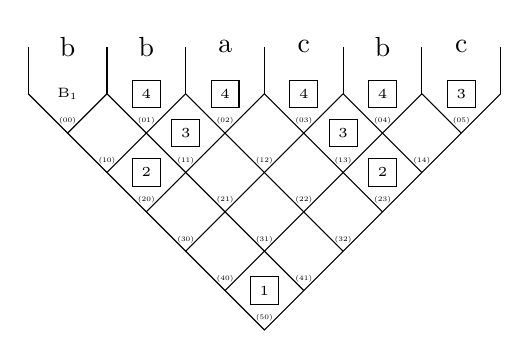
\begin{tikzpicture}[baseline]
				\newcommand{\myfontvars}[1]{
					\fontsize{4.9}{12}\selectfont{#1}
				}\newcommand{\myfontnumbering}[1]{
					\fontsize{2.5}{12}\selectfont{#1}
				}%Outer hull
				%Tip of the pyramid
				\coordinate (tip) at (3.0,-3.0);
				\foreach \i in {0,...,6} {
					\coordinate (\i) at (\i,0);
				}
				%Draw the left and right line of the pyramid pointing downwards
				\draw (0) -- (tip) -- (6);
				%Grid lines direction down-left to top-right
				\coordinate (dl1) at (0.5,-0.5);
				\coordinate (dl2) at (1.0,-1.0);
				\coordinate (dl3) at (1.5,-1.5);
				\coordinate (dl4) at (2.0,-2.0);
				\coordinate (dl5) at (2.5,-2.5);
				\draw (dl1) -- (1,0);
				\draw (dl2) -- (2,0);
				\draw (dl3) -- (3,0);
				\draw (dl4) -- (4,0);
				\draw (dl5) -- (5,0);
				%Grid lines direction down-right to top-left
				\coordinate (dr1) at (3.5,-2.5);
				\coordinate (dr2) at (4.0,-2.0);
				\coordinate (dr3) at (4.5,-1.5);
				\coordinate (dr4) at (5.0,-1.0);
				\coordinate (dr5) at (5.5,-0.5);
				\draw (dr1) -- (1,0);
				\draw (dr2) -- (2,0);
				\draw (dr3) -- (3,0);
				\draw (dr4) -- (4,0);
				\draw (dr5) -- (5,0);
				%Small lines at the top
				\coordinate (top0) at (0.0,0.0);
				\coordinate (top1) at (1.0,0.0);
				\coordinate (top2) at (2.0,0.0);
				\coordinate (top3) at (3.0,0.0);
				\coordinate (top4) at (4.0,0.0);
				\coordinate (top5) at (5.0,0.0);
				\coordinate (top6) at (6.0,0.0);
				\coordinate (topUpper0) at (0.0,0.6);
				\coordinate (topUpper1) at (1.0,0.6);
				\coordinate (topUpper2) at (2.0,0.6);
				\coordinate (topUpper3) at (3.0,0.6);
				\coordinate (topUpper4) at (4.0,0.6);
				\coordinate (topUpper5) at (5.0,0.6);
				\coordinate (topUpper6) at (6.0,0.6);
				\draw (top0) -- (topUpper0);
				\draw (top1) -- (topUpper1);
				\draw (top2) -- (topUpper2);
				\draw (top3) -- (topUpper3);
				\draw (top4) -- (topUpper4);
				\draw (top5) -- (topUpper5);
				\draw (top6) -- (topUpper6);
				%The string
				\coordinate (w0) at (0.5,0.6);
				\coordinate (w1) at (1.5,0.6);
				\coordinate (w2) at (2.5,0.6);
				\coordinate (w3) at (3.5,0.6);
				\coordinate (w4) at (4.5,0.6);
				\coordinate (w5) at (5.5,0.6);
				\node [] at (w0) {b};
				\node [] at (w1) {b};
				\node [] at (w2) {a};
				\node [] at (w3) {c};
				\node [] at (w4) {b};
				\node [] at (w5) {c};
				% Variables in the cells
				%cells00
				\coordinate (center00) at (0.5,0.0);
				\node [below=0.18cm] at (center00) {\myfontnumbering{$(00)$}};
				\node [] at (center00) {\myfontvars{B$_{1}$}};
				%cells01
				\coordinate (center01) at (1.5,0.0);
				\node [below=0.18cm] at (center01) {\myfontnumbering{$(01)$}};
				\node [] at (center01) [minimum height=0.25cm,minimum width=0.25cm,draw] {\tiny{4}};
				%cells02
				\coordinate (center02) at (2.5,0.0);
				\node [below=0.18cm] at (center02) {\myfontnumbering{$(02)$}};
				\node [] at (center02) [minimum height=0.25cm,minimum width=0.25cm,draw] {\tiny{4}};
				%cells03
				\coordinate (center03) at (3.5,0.0);
				\node [below=0.18cm] at (center03) {\myfontnumbering{$(03)$}};
				\node [] at (center03) [minimum height=0.25cm,minimum width=0.25cm,draw] {\tiny{4}};
				%cells04
				\coordinate (center04) at (4.5,0.0);
				\node [below=0.18cm] at (center04) {\myfontnumbering{$(04)$}};
				\node [] at (center04) [minimum height=0.25cm,minimum width=0.25cm,draw] {\tiny{4}};
				%cells05
				\coordinate (center05) at (5.5,0.0);
				\node [below=0.18cm] at (center05) {\myfontnumbering{$(05)$}};
				\node [] at (center05) [minimum height=0.25cm,minimum width=0.25cm,draw] {\tiny{3}};
				%cells10
				\coordinate (center10) at (1.0,-0.5);
				\node [below=0.18cm] at (center10) {\myfontnumbering{$(10)$}};
				%cells11
				\coordinate (center11) at (2.0,-0.5);
				\node [below=0.18cm] at (center11) {\myfontnumbering{$(11)$}};
				\node [] at (center11) [minimum height=0.25cm,minimum width=0.25cm,draw] {\tiny{3}};
				%cells12
				\coordinate (center12) at (3.0,-0.5);
				\node [below=0.18cm] at (center12) {\myfontnumbering{$(12)$}};
				%cells13
				\coordinate (center13) at (4.0,-0.5);
				\node [below=0.18cm] at (center13) {\myfontnumbering{$(13)$}};
				\node [] at (center13) [minimum height=0.25cm,minimum width=0.25cm,draw] {\tiny{3}};
				%cells14
				\coordinate (center14) at (5.0,-0.5);
				\node [below=0.18cm] at (center14) {\myfontnumbering{$(14)$}};
				%cells20
				\coordinate (center20) at (1.5,-1.0);
				\node [below=0.18cm] at (center20) {\myfontnumbering{$(20)$}};
				\node [] at (center20) [minimum height=0.25cm,minimum width=0.25cm,draw] {\tiny{2}};
				%cells21
				\coordinate (center21) at (2.5,-1.0);
				\node [below=0.18cm] at (center21) {\myfontnumbering{$(21)$}};
				%cells22
				\coordinate (center22) at (3.5,-1.0);
				\node [below=0.18cm] at (center22) {\myfontnumbering{$(22)$}};
				%cells23
				\coordinate (center23) at (4.5,-1.0);
				\node [below=0.18cm] at (center23) {\myfontnumbering{$(23)$}};
				\node [] at (center23) [minimum height=0.25cm,minimum width=0.25cm,draw] {\tiny{2}};
				%cells30
				\coordinate (center30) at (2.0,-1.5);
				\node [below=0.18cm] at (center30) {\myfontnumbering{$(30)$}};
				%cells31
				\coordinate (center31) at (3.0,-1.5);
				\node [below=0.18cm] at (center31) {\myfontnumbering{$(31)$}};
				%cells32
				\coordinate (center32) at (4.0,-1.5);
				\node [below=0.18cm] at (center32) {\myfontnumbering{$(32)$}};
				%cells40
				\coordinate (center40) at (2.5,-2.0);
				\node [below=0.18cm] at (center40) {\myfontnumbering{$(40)$}};
				%cells41
				\coordinate (center41) at (3.5,-2.0);
				\node [below=0.18cm] at (center41) {\myfontnumbering{$(41)$}};
				%cells50
				\coordinate (center50) at (3.0,-2.5);
				\node [below=0.18cm] at (center50) {\myfontnumbering{$(50)$}};
				\node [] at (center50) [minimum height=0.25cm,minimum width=0.25cm,draw] {\tiny{1}};
				\end{tikzpicture}
			}
	\end{minipage}
	\captionof{figure}{Illustration of Algorithm \ref{SplitAndFill} part 1. To resolve the recursion step that fills $Cell_{0,0}$ the rule $B\rightarrow b$ is added.}
	\label{IllustrationAlgorithmSplitAndFillPart1}
	
	\noindent At first the rule $B\longrightarrow b$ is added as shown in Figure \ref{IllustrationAlgorithmSplitAndFillPart1}.\\ Next are the rules $A\longrightarrow a$ and $S\longrightarrow BA$ as seen in Figure \ref{IllustrationAlgorithmSplitAndFillPart2}. To resolve the recursion step that fills $Cell_{0,1}$ no rule is added because a rule $lhse\rightarrow b$ already exists. To fill $Cell_{0,2}$ the rule $A\rightarrow a$ and regarding $Cell_{1,1}$ the rule $S \rightarrow BA$ is added.\\
	
	
	\begin{minipage}{6in}
		\centering
		\begin{tabular}{l}
			Grammar:\\
			$A \rightarrow \textbf{a}$\\
			$B \rightarrow b$\\ 
			$C \rightarrow $\\
			$S \rightarrow \textbf{BA}$\\ 
		\end{tabular} 
		\resizebox{0.65\linewidth}{!}{
			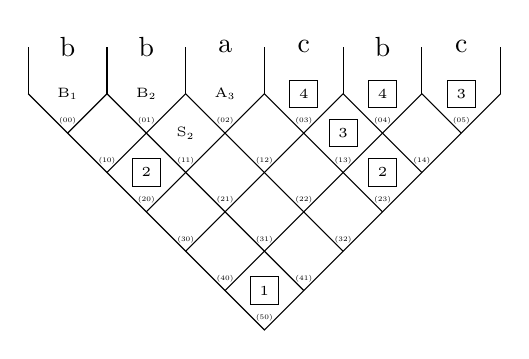
\begin{tikzpicture}[baseline]
			\newcommand{\myfontvars}[1]{
				\fontsize{4.9}{12}\selectfont{#1}
			}\newcommand{\myfontnumbering}[1]{
				\fontsize{2.5}{12}\selectfont{#1}
			}%Outer hull
			%Tip of the pyramid
			\coordinate (tip) at (3.0,-3.0);
			\foreach \i in {0,...,6} {
				\coordinate (\i) at (\i,0);
			}
			%Draw the left and right line of the pyramid pointing downwards
			\draw (0) -- (tip) -- (6);
			%Grid lines direction down-left to top-right
			\coordinate (dl1) at (0.5,-0.5);
			\coordinate (dl2) at (1.0,-1.0);
			\coordinate (dl3) at (1.5,-1.5);
			\coordinate (dl4) at (2.0,-2.0);
			\coordinate (dl5) at (2.5,-2.5);
			\draw (dl1) -- (1,0);
			\draw (dl2) -- (2,0);
			\draw (dl3) -- (3,0);
			\draw (dl4) -- (4,0);
			\draw (dl5) -- (5,0);
			%Grid lines direction down-right to top-left
			\coordinate (dr1) at (3.5,-2.5);
			\coordinate (dr2) at (4.0,-2.0);
			\coordinate (dr3) at (4.5,-1.5);
			\coordinate (dr4) at (5.0,-1.0);
			\coordinate (dr5) at (5.5,-0.5);
			\draw (dr1) -- (1,0);
			\draw (dr2) -- (2,0);
			\draw (dr3) -- (3,0);
			\draw (dr4) -- (4,0);
			\draw (dr5) -- (5,0);
			%Small lines at the top
			\coordinate (top0) at (0.0,0.0);
			\coordinate (top1) at (1.0,0.0);
			\coordinate (top2) at (2.0,0.0);
			\coordinate (top3) at (3.0,0.0);
			\coordinate (top4) at (4.0,0.0);
			\coordinate (top5) at (5.0,0.0);
			\coordinate (top6) at (6.0,0.0);
			\coordinate (topUpper0) at (0.0,0.6);
			\coordinate (topUpper1) at (1.0,0.6);
			\coordinate (topUpper2) at (2.0,0.6);
			\coordinate (topUpper3) at (3.0,0.6);
			\coordinate (topUpper4) at (4.0,0.6);
			\coordinate (topUpper5) at (5.0,0.6);
			\coordinate (topUpper6) at (6.0,0.6);
			\draw (top0) -- (topUpper0);
			\draw (top1) -- (topUpper1);
			\draw (top2) -- (topUpper2);
			\draw (top3) -- (topUpper3);
			\draw (top4) -- (topUpper4);
			\draw (top5) -- (topUpper5);
			\draw (top6) -- (topUpper6);
			%The string
			\coordinate (w0) at (0.5,0.6);
			\coordinate (w1) at (1.5,0.6);
			\coordinate (w2) at (2.5,0.6);
			\coordinate (w3) at (3.5,0.6);
			\coordinate (w4) at (4.5,0.6);
			\coordinate (w5) at (5.5,0.6);
			\node [] at (w0) {b};
			\node [] at (w1) {b};
			\node [] at (w2) {a};
			\node [] at (w3) {c};
			\node [] at (w4) {b};
			\node [] at (w5) {c};
			% Variables in the cells
			%cells00
			\coordinate (center00) at (0.5,0.0);
			\node [below=0.18cm] at (center00) {\myfontnumbering{$(00)$}};
			\node [] at (center00) {\myfontvars{B$_{1}$}};
			%cells01
			\coordinate (center01) at (1.5,0.0);
			\node [below=0.18cm] at (center01) {\myfontnumbering{$(01)$}};
			\node [] at (center01) {\myfontvars{B$_{2}$}};
			%cells02
			\coordinate (center02) at (2.5,0.0);
			\node [below=0.18cm] at (center02) {\myfontnumbering{$(02)$}};
			\node [] at (center02) {\myfontvars{A$_{3}$}};
			%cells03
			\coordinate (center03) at (3.5,0.0);
			\node [below=0.18cm] at (center03) {\myfontnumbering{$(03)$}};
			\node [] at (center03) [minimum height=0.25cm,minimum width=0.25cm,draw] {\tiny{4}};
			%cells04
			\coordinate (center04) at (4.5,0.0);
			\node [below=0.18cm] at (center04) {\myfontnumbering{$(04)$}};
			\node [] at (center04) [minimum height=0.25cm,minimum width=0.25cm,draw] {\tiny{4}};
			%cells05
			\coordinate (center05) at (5.5,0.0);
			\node [below=0.18cm] at (center05) {\myfontnumbering{$(05)$}};
			\node [] at (center05) [minimum height=0.25cm,minimum width=0.25cm,draw] {\tiny{3}};
			%cells10
			\coordinate (center10) at (1.0,-0.5);
			\node [below=0.18cm] at (center10) {\myfontnumbering{$(10)$}};
			%cells11
			\coordinate (center11) at (2.0,-0.5);
			\node [below=0.18cm] at (center11) {\myfontnumbering{$(11)$}};
			\node [] at (center11) {\myfontvars{S$_{2}$}};
			%cells12
			\coordinate (center12) at (3.0,-0.5);
			\node [below=0.18cm] at (center12) {\myfontnumbering{$(12)$}};
			%cells13
			\coordinate (center13) at (4.0,-0.5);
			\node [below=0.18cm] at (center13) {\myfontnumbering{$(13)$}};
			\node [] at (center13) [minimum height=0.25cm,minimum width=0.25cm,draw] {\tiny{3}};
			%cells14
			\coordinate (center14) at (5.0,-0.5);
			\node [below=0.18cm] at (center14) {\myfontnumbering{$(14)$}};
			%cells20
			\coordinate (center20) at (1.5,-1.0);
			\node [below=0.18cm] at (center20) {\myfontnumbering{$(20)$}};
			\node [] at (center20) [minimum height=0.25cm,minimum width=0.25cm,draw] {\tiny{2}};
			%cells21
			\coordinate (center21) at (2.5,-1.0);
			\node [below=0.18cm] at (center21) {\myfontnumbering{$(21)$}};
			%cells22
			\coordinate (center22) at (3.5,-1.0);
			\node [below=0.18cm] at (center22) {\myfontnumbering{$(22)$}};
			%cells23
			\coordinate (center23) at (4.5,-1.0);
			\node [below=0.18cm] at (center23) {\myfontnumbering{$(23)$}};
			\node [] at (center23) [minimum height=0.25cm,minimum width=0.25cm,draw] {\tiny{2}};
			%cells30
			\coordinate (center30) at (2.0,-1.5);
			\node [below=0.18cm] at (center30) {\myfontnumbering{$(30)$}};
			%cells31
			\coordinate (center31) at (3.0,-1.5);
			\node [below=0.18cm] at (center31) {\myfontnumbering{$(31)$}};
			%cells32
			\coordinate (center32) at (4.0,-1.5);
			\node [below=0.18cm] at (center32) {\myfontnumbering{$(32)$}};
			%cells40
			\coordinate (center40) at (2.5,-2.0);
			\node [below=0.18cm] at (center40) {\myfontnumbering{$(40)$}};
			%cells41
			\coordinate (center41) at (3.5,-2.0);
			\node [below=0.18cm] at (center41) {\myfontnumbering{$(41)$}};
			%cells50
			\coordinate (center50) at (3.0,-2.5);
			\node [below=0.18cm] at (center50) {\myfontnumbering{$(50)$}};
			\node [] at (center50) [minimum height=0.25cm,minimum width=0.25cm,draw] {\tiny{1}};
			\end{tikzpicture}
		}
	\end{minipage}
	\captionof{figure}{Illustration of Algorithm \ref{SplitAndFill} part 2. Adding of the rules $A\longrightarrow a$ and $S\longrightarrow BA$.}
	\label{IllustrationAlgorithmSplitAndFillPart2}
	~\\
	To fill the $Cell_{2,0}$ the rule $C \rightarrow BS$ is added, see Figure \ref{IllustrationAlgorithmSplitAndFillPart3}: \\
	
	\begin{minipage}{6in}
		\centering
		\begin{tabular}{l}
			Grammar:\\
			$A \rightarrow a$\\
			$B \rightarrow b$\\ 
			$C \rightarrow \textbf{BS}$\\
			$S \rightarrow BA$\\ 
		\end{tabular} 
		\resizebox{0.65\linewidth}{!}{
			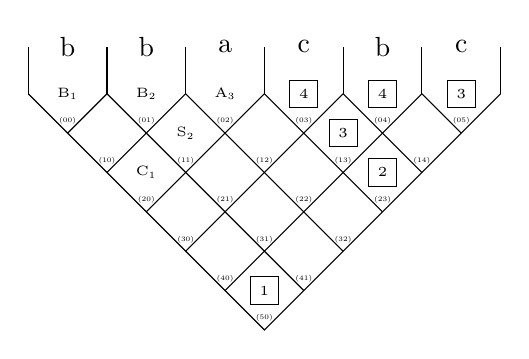
\begin{tikzpicture}[baseline]
			\newcommand{\myfontvars}[1]{
				\fontsize{4.9}{12}\selectfont{#1}
			}\newcommand{\myfontnumbering}[1]{
				\fontsize{2.5}{12}\selectfont{#1}
			}%Outer hull
			%Tip of the pyramid
			\coordinate (tip) at (3.0,-3.0);
			\foreach \i in {0,...,6} {
				\coordinate (\i) at (\i,0);
			}
			%Draw the left and right line of the pyramid pointing downwards
			\draw (0) -- (tip) -- (6);
			%Grid lines direction down-left to top-right
			\coordinate (dl1) at (0.5,-0.5);
			\coordinate (dl2) at (1.0,-1.0);
			\coordinate (dl3) at (1.5,-1.5);
			\coordinate (dl4) at (2.0,-2.0);
			\coordinate (dl5) at (2.5,-2.5);
			\draw (dl1) -- (1,0);
			\draw (dl2) -- (2,0);
			\draw (dl3) -- (3,0);
			\draw (dl4) -- (4,0);
			\draw (dl5) -- (5,0);
			%Grid lines direction down-right to top-left
			\coordinate (dr1) at (3.5,-2.5);
			\coordinate (dr2) at (4.0,-2.0);
			\coordinate (dr3) at (4.5,-1.5);
			\coordinate (dr4) at (5.0,-1.0);
			\coordinate (dr5) at (5.5,-0.5);
			\draw (dr1) -- (1,0);
			\draw (dr2) -- (2,0);
			\draw (dr3) -- (3,0);
			\draw (dr4) -- (4,0);
			\draw (dr5) -- (5,0);
			%Small lines at the top
			\coordinate (top0) at (0.0,0.0);
			\coordinate (top1) at (1.0,0.0);
			\coordinate (top2) at (2.0,0.0);
			\coordinate (top3) at (3.0,0.0);
			\coordinate (top4) at (4.0,0.0);
			\coordinate (top5) at (5.0,0.0);
			\coordinate (top6) at (6.0,0.0);
			\coordinate (topUpper0) at (0.0,0.6);
			\coordinate (topUpper1) at (1.0,0.6);
			\coordinate (topUpper2) at (2.0,0.6);
			\coordinate (topUpper3) at (3.0,0.6);
			\coordinate (topUpper4) at (4.0,0.6);
			\coordinate (topUpper5) at (5.0,0.6);
			\coordinate (topUpper6) at (6.0,0.6);
			\draw (top0) -- (topUpper0);
			\draw (top1) -- (topUpper1);
			\draw (top2) -- (topUpper2);
			\draw (top3) -- (topUpper3);
			\draw (top4) -- (topUpper4);
			\draw (top5) -- (topUpper5);
			\draw (top6) -- (topUpper6);
			%The string
			\coordinate (w0) at (0.5,0.6);
			\coordinate (w1) at (1.5,0.6);
			\coordinate (w2) at (2.5,0.6);
			\coordinate (w3) at (3.5,0.6);
			\coordinate (w4) at (4.5,0.6);
			\coordinate (w5) at (5.5,0.6);
			\node [] at (w0) {b};
			\node [] at (w1) {b};
			\node [] at (w2) {a};
			\node [] at (w3) {c};
			\node [] at (w4) {b};
			\node [] at (w5) {c};
			% Variables in the cells
			%cells00
			\coordinate (center00) at (0.5,0.0);
			\node [below=0.18cm] at (center00) {\myfontnumbering{$(00)$}};
			\node [] at (center00) {\myfontvars{B$_{1}$}};
			%cells01
			\coordinate (center01) at (1.5,0.0);
			\node [below=0.18cm] at (center01) {\myfontnumbering{$(01)$}};
			\node [] at (center01) {\myfontvars{B$_{2}$}};
			%cells02
			\coordinate (center02) at (2.5,0.0);
			\node [below=0.18cm] at (center02) {\myfontnumbering{$(02)$}};
			\node [] at (center02) {\myfontvars{A$_{3}$}};
			%cells03
			\coordinate (center03) at (3.5,0.0);
			\node [below=0.18cm] at (center03) {\myfontnumbering{$(03)$}};
			\node [] at (center03) [minimum height=0.25cm,minimum width=0.25cm,draw] {\tiny{4}};
			%cells04
			\coordinate (center04) at (4.5,0.0);
			\node [below=0.18cm] at (center04) {\myfontnumbering{$(04)$}};
			\node [] at (center04) [minimum height=0.25cm,minimum width=0.25cm,draw] {\tiny{4}};
			%cells05
			\coordinate (center05) at (5.5,0.0);
			\node [below=0.18cm] at (center05) {\myfontnumbering{$(05)$}};
			\node [] at (center05) [minimum height=0.25cm,minimum width=0.25cm,draw] {\tiny{3}};
			%cells10
			\coordinate (center10) at (1.0,-0.5);
			\node [below=0.18cm] at (center10) {\myfontnumbering{$(10)$}};
			%cells11
			\coordinate (center11) at (2.0,-0.5);
			\node [below=0.18cm] at (center11) {\myfontnumbering{$(11)$}};
			\node [] at (center11) {\myfontvars{S$_{2}$}};
			%cells12
			\coordinate (center12) at (3.0,-0.5);
			\node [below=0.18cm] at (center12) {\myfontnumbering{$(12)$}};
			%cells13
			\coordinate (center13) at (4.0,-0.5);
			\node [below=0.18cm] at (center13) {\myfontnumbering{$(13)$}};
			\node [] at (center13) [minimum height=0.25cm,minimum width=0.25cm,draw] {\tiny{3}};
			%cells14
			\coordinate (center14) at (5.0,-0.5);
			\node [below=0.18cm] at (center14) {\myfontnumbering{$(14)$}};
			%cells20
			\coordinate (center20) at (1.5,-1.0);
			\node [below=0.18cm] at (center20) {\myfontnumbering{$(20)$}};
			\node [] at (center20) {\myfontvars{C$_{1}$}};
			%cells21
			\coordinate (center21) at (2.5,-1.0);
			\node [below=0.18cm] at (center21) {\myfontnumbering{$(21)$}};
			%cells22
			\coordinate (center22) at (3.5,-1.0);
			\node [below=0.18cm] at (center22) {\myfontnumbering{$(22)$}};
			%cells23
			\coordinate (center23) at (4.5,-1.0);
			\node [below=0.18cm] at (center23) {\myfontnumbering{$(23)$}};
			\node [] at (center23) [minimum height=0.25cm,minimum width=0.25cm,draw] {\tiny{2}};
			%cells30
			\coordinate (center30) at (2.0,-1.5);
			\node [below=0.18cm] at (center30) {\myfontnumbering{$(30)$}};
			%cells31
			\coordinate (center31) at (3.0,-1.5);
			\node [below=0.18cm] at (center31) {\myfontnumbering{$(31)$}};
			%cells32
			\coordinate (center32) at (4.0,-1.5);
			\node [below=0.18cm] at (center32) {\myfontnumbering{$(32)$}};
			%cells40
			\coordinate (center40) at (2.5,-2.0);
			\node [below=0.18cm] at (center40) {\myfontnumbering{$(40)$}};
			%cells41
			\coordinate (center41) at (3.5,-2.0);
			\node [below=0.18cm] at (center41) {\myfontnumbering{$(41)$}};
			%cells50
			\coordinate (center50) at (3.0,-2.5);
			\node [below=0.18cm] at (center50) {\myfontnumbering{$(50)$}};
			\node [] at (center50) [minimum height=0.25cm,minimum width=0.25cm,draw] {\tiny{1}};
			\end{tikzpicture}
		}
	\end{minipage}
	\captionof{figure}{Illustration of Algorithm \ref{SplitAndFill} part 3. Adding of the rule $C \rightarrow BS$ to fill the $Cell_{2,0}$.}
	\label{IllustrationAlgorithmSplitAndFillPart3}
	\pagebreak
	
	\noindent Analogously the other cells are filled. $Cell_{0,3}$ is responsible for the rule $C \rightarrow c$, $Cell_{0,4}$ doesn't cause a rule because again there already is the rule $B \rightarrow b$, $Cell_{1,3}$ contributes for the rule $B \rightarrow CB$, $Cell_{0,5}$ does not add a rule because of $C\rightarrow c$ and to fill $Cell_{2,3}$ the rule $A \rightarrow BC$ is added.\\
	
	\begin{minipage}{6in}
		\centering
		\begin{tabular}{l}
			Grammar:\\
			$A \rightarrow \textbf{BC}~|~a$\\
			$B \rightarrow \textbf{CB}~|~b$\\ 
			$C \rightarrow BS~|~c$\\
			$S \rightarrow BA$\\ 
		\end{tabular} 
		\resizebox{0.65\linewidth}{!}{
			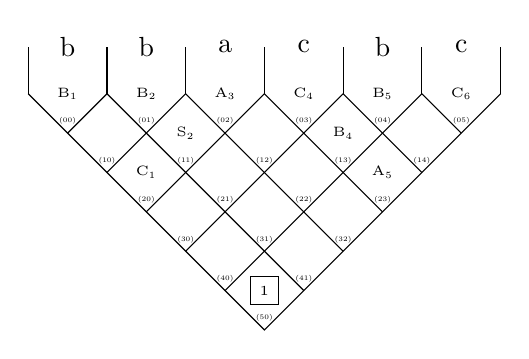
\begin{tikzpicture}[baseline]
			\newcommand{\myfontvars}[1]{
				\fontsize{4.9}{12}\selectfont{#1}
			}\newcommand{\myfontnumbering}[1]{
				\fontsize{2.5}{12}\selectfont{#1}
			}%Outer hull
			%Tip of the pyramid
			\coordinate (tip) at (3.0,-3.0);
			\foreach \i in {0,...,6} {
				\coordinate (\i) at (\i,0);
			}
			%Draw the left and right line of the pyramid pointing downwards
			\draw (0) -- (tip) -- (6);
			%Grid lines direction down-left to top-right
			\coordinate (dl1) at (0.5,-0.5);
			\coordinate (dl2) at (1.0,-1.0);
			\coordinate (dl3) at (1.5,-1.5);
			\coordinate (dl4) at (2.0,-2.0);
			\coordinate (dl5) at (2.5,-2.5);
			\draw (dl1) -- (1,0);
			\draw (dl2) -- (2,0);
			\draw (dl3) -- (3,0);
			\draw (dl4) -- (4,0);
			\draw (dl5) -- (5,0);
			%Grid lines direction down-right to top-left
			\coordinate (dr1) at (3.5,-2.5);
			\coordinate (dr2) at (4.0,-2.0);
			\coordinate (dr3) at (4.5,-1.5);
			\coordinate (dr4) at (5.0,-1.0);
			\coordinate (dr5) at (5.5,-0.5);
			\draw (dr1) -- (1,0);
			\draw (dr2) -- (2,0);
			\draw (dr3) -- (3,0);
			\draw (dr4) -- (4,0);
			\draw (dr5) -- (5,0);
			%Small lines at the top
			\coordinate (top0) at (0.0,0.0);
			\coordinate (top1) at (1.0,0.0);
			\coordinate (top2) at (2.0,0.0);
			\coordinate (top3) at (3.0,0.0);
			\coordinate (top4) at (4.0,0.0);
			\coordinate (top5) at (5.0,0.0);
			\coordinate (top6) at (6.0,0.0);
			\coordinate (topUpper0) at (0.0,0.6);
			\coordinate (topUpper1) at (1.0,0.6);
			\coordinate (topUpper2) at (2.0,0.6);
			\coordinate (topUpper3) at (3.0,0.6);
			\coordinate (topUpper4) at (4.0,0.6);
			\coordinate (topUpper5) at (5.0,0.6);
			\coordinate (topUpper6) at (6.0,0.6);
			\draw (top0) -- (topUpper0);
			\draw (top1) -- (topUpper1);
			\draw (top2) -- (topUpper2);
			\draw (top3) -- (topUpper3);
			\draw (top4) -- (topUpper4);
			\draw (top5) -- (topUpper5);
			\draw (top6) -- (topUpper6);
			%The string
			\coordinate (w0) at (0.5,0.6);
			\coordinate (w1) at (1.5,0.6);
			\coordinate (w2) at (2.5,0.6);
			\coordinate (w3) at (3.5,0.6);
			\coordinate (w4) at (4.5,0.6);
			\coordinate (w5) at (5.5,0.6);
			\node [] at (w0) {b};
			\node [] at (w1) {b};
			\node [] at (w2) {a};
			\node [] at (w3) {c};
			\node [] at (w4) {b};
			\node [] at (w5) {c};
			% Variables in the cells
			%cells00
			\coordinate (center00) at (0.5,0.0);
			\node [below=0.18cm] at (center00) {\myfontnumbering{$(00)$}};
			\node [] at (center00) {\myfontvars{B$_{1}$}};
			%cells01
			\coordinate (center01) at (1.5,0.0);
			\node [below=0.18cm] at (center01) {\myfontnumbering{$(01)$}};
			\node [] at (center01) {\myfontvars{B$_{2}$}};
			%cells02
			\coordinate (center02) at (2.5,0.0);
			\node [below=0.18cm] at (center02) {\myfontnumbering{$(02)$}};
			\node [] at (center02) {\myfontvars{A$_{3}$}};
			%cells03
			\coordinate (center03) at (3.5,0.0);
			\node [below=0.18cm] at (center03) {\myfontnumbering{$(03)$}};
			\node [] at (center03) {\myfontvars{C$_{4}$}};
			%cells04
			\coordinate (center04) at (4.5,0.0);
			\node [below=0.18cm] at (center04) {\myfontnumbering{$(04)$}};
			\node [] at (center04) {\myfontvars{B$_{5}$}};
			%cells05
			\coordinate (center05) at (5.5,0.0);
			\node [below=0.18cm] at (center05) {\myfontnumbering{$(05)$}};
			\node [] at (center05) {\myfontvars{C$_{6}$}};
			%cells10
			\coordinate (center10) at (1.0,-0.5);
			\node [below=0.18cm] at (center10) {\myfontnumbering{$(10)$}};
			%cells11
			\coordinate (center11) at (2.0,-0.5);
			\node [below=0.18cm] at (center11) {\myfontnumbering{$(11)$}};
			\node [] at (center11) {\myfontvars{S$_{2}$}};
			%cells12
			\coordinate (center12) at (3.0,-0.5);
			\node [below=0.18cm] at (center12) {\myfontnumbering{$(12)$}};
			%cells13
			\coordinate (center13) at (4.0,-0.5);
			\node [below=0.18cm] at (center13) {\myfontnumbering{$(13)$}};
			\node [] at (center13) {\myfontvars{B$_{4}$}};
			%cells14
			\coordinate (center14) at (5.0,-0.5);
			\node [below=0.18cm] at (center14) {\myfontnumbering{$(14)$}};
			%cells20
			\coordinate (center20) at (1.5,-1.0);
			\node [below=0.18cm] at (center20) {\myfontnumbering{$(20)$}};
			\node [] at (center20) {\myfontvars{C$_{1}$}};
			%cells21
			\coordinate (center21) at (2.5,-1.0);
			\node [below=0.18cm] at (center21) {\myfontnumbering{$(21)$}};
			%cells22
			\coordinate (center22) at (3.5,-1.0);
			\node [below=0.18cm] at (center22) {\myfontnumbering{$(22)$}};
			%cells23
			\coordinate (center23) at (4.5,-1.0);
			\node [below=0.18cm] at (center23) {\myfontnumbering{$(23)$}};
			\node [] at (center23) {\myfontvars{A$_{5}$}};
			%cells30
			\coordinate (center30) at (2.0,-1.5);
			\node [below=0.18cm] at (center30) {\myfontnumbering{$(30)$}};
			%cells31
			\coordinate (center31) at (3.0,-1.5);
			\node [below=0.18cm] at (center31) {\myfontnumbering{$(31)$}};
			%cells32
			\coordinate (center32) at (4.0,-1.5);
			\node [below=0.18cm] at (center32) {\myfontnumbering{$(32)$}};
			%cells40
			\coordinate (center40) at (2.5,-2.0);
			\node [below=0.18cm] at (center40) {\myfontnumbering{$(40)$}};
			%cells41
			\coordinate (center41) at (3.5,-2.0);
			\node [below=0.18cm] at (center41) {\myfontnumbering{$(41)$}};
			%cells50
			\coordinate (center50) at (3.0,-2.5);
			\node [below=0.18cm] at (center50) {\myfontnumbering{$(50)$}};
			\node [] at (center50) [minimum height=0.25cm,minimum width=0.25cm,draw] {\tiny{1}};
			\end{tikzpicture}
		}
	\end{minipage}
	\captionof{figure}{Illustration of Algorithm \ref{SplitAndFill} part 4. Adding of the rules $A\longrightarrow BC$ and $B \longrightarrow CB$.}
	\label{IllustrationAlgorithmSplitAndFillPart4}
	~\\
	\noindent To fill the cell in the root a rule must be added that has the start variable as its $lhse$ that guarantees $w \in L(G)$. Here the rule $S\rightarrow CA$ is added.\\

	\begin{minipage}{6in}
		\centering
		\begin{tabular}{l}
			Grammar:\\
			$A \rightarrow BC~|~a$\\
			$B \rightarrow CB~|~b$\\ 
			$C \rightarrow BS~|~c$\\
			$S \rightarrow BA~|~\textbf{CA}$\\ 
		\end{tabular} 
		\resizebox{0.65\linewidth}{!}{
			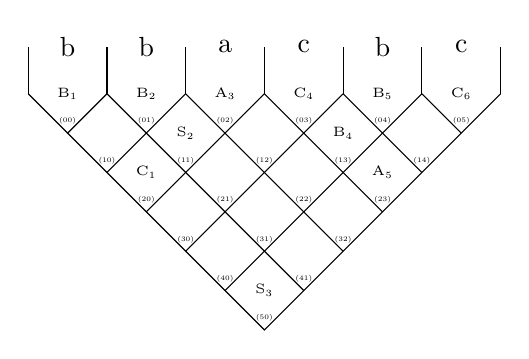
\begin{tikzpicture}[baseline]
			\newcommand{\myfontvars}[1]{
				\fontsize{4.9}{12}\selectfont{#1}
			}\newcommand{\myfontnumbering}[1]{
				\fontsize{2.5}{12}\selectfont{#1}
			}%Outer hull
			%Tip of the pyramid
			\coordinate (tip) at (3.0,-3.0);
			\foreach \i in {0,...,6} {
				\coordinate (\i) at (\i,0);
			}
			%Draw the left and right line of the pyramid pointing downwards
			\draw (0) -- (tip) -- (6);
			%Grid lines direction down-left to top-right
			\coordinate (dl1) at (0.5,-0.5);
			\coordinate (dl2) at (1.0,-1.0);
			\coordinate (dl3) at (1.5,-1.5);
			\coordinate (dl4) at (2.0,-2.0);
			\coordinate (dl5) at (2.5,-2.5);
			\draw (dl1) -- (1,0);
			\draw (dl2) -- (2,0);
			\draw (dl3) -- (3,0);
			\draw (dl4) -- (4,0);
			\draw (dl5) -- (5,0);
			%Grid lines direction down-right to top-left
			\coordinate (dr1) at (3.5,-2.5);
			\coordinate (dr2) at (4.0,-2.0);
			\coordinate (dr3) at (4.5,-1.5);
			\coordinate (dr4) at (5.0,-1.0);
			\coordinate (dr5) at (5.5,-0.5);
			\draw (dr1) -- (1,0);
			\draw (dr2) -- (2,0);
			\draw (dr3) -- (3,0);
			\draw (dr4) -- (4,0);
			\draw (dr5) -- (5,0);
			%Small lines at the top
			\coordinate (top0) at (0.0,0.0);
			\coordinate (top1) at (1.0,0.0);
			\coordinate (top2) at (2.0,0.0);
			\coordinate (top3) at (3.0,0.0);
			\coordinate (top4) at (4.0,0.0);
			\coordinate (top5) at (5.0,0.0);
			\coordinate (top6) at (6.0,0.0);
			\coordinate (topUpper0) at (0.0,0.6);
			\coordinate (topUpper1) at (1.0,0.6);
			\coordinate (topUpper2) at (2.0,0.6);
			\coordinate (topUpper3) at (3.0,0.6);
			\coordinate (topUpper4) at (4.0,0.6);
			\coordinate (topUpper5) at (5.0,0.6);
			\coordinate (topUpper6) at (6.0,0.6);
			\draw (top0) -- (topUpper0);
			\draw (top1) -- (topUpper1);
			\draw (top2) -- (topUpper2);
			\draw (top3) -- (topUpper3);
			\draw (top4) -- (topUpper4);
			\draw (top5) -- (topUpper5);
			\draw (top6) -- (topUpper6);
			%The string
			\coordinate (w0) at (0.5,0.6);
			\coordinate (w1) at (1.5,0.6);
			\coordinate (w2) at (2.5,0.6);
			\coordinate (w3) at (3.5,0.6);
			\coordinate (w4) at (4.5,0.6);
			\coordinate (w5) at (5.5,0.6);
			\node [] at (w0) {b};
			\node [] at (w1) {b};
			\node [] at (w2) {a};
			\node [] at (w3) {c};
			\node [] at (w4) {b};
			\node [] at (w5) {c};
			% Variables in the cells
			%cells00
			\coordinate (center00) at (0.5,0.0);
			\node [below=0.18cm] at (center00) {\myfontnumbering{$(00)$}};
			\node [] at (center00) {\myfontvars{B$_{1}$}};
			%cells01
			\coordinate (center01) at (1.5,0.0);
			\node [below=0.18cm] at (center01) {\myfontnumbering{$(01)$}};
			\node [] at (center01) {\myfontvars{B$_{2}$}};
			%cells02
			\coordinate (center02) at (2.5,0.0);
			\node [below=0.18cm] at (center02) {\myfontnumbering{$(02)$}};
			\node [] at (center02) {\myfontvars{A$_{3}$}};
			%cells03
			\coordinate (center03) at (3.5,0.0);
			\node [below=0.18cm] at (center03) {\myfontnumbering{$(03)$}};
			\node [] at (center03) {\myfontvars{C$_{4}$}};
			%cells04
			\coordinate (center04) at (4.5,0.0);
			\node [below=0.18cm] at (center04) {\myfontnumbering{$(04)$}};
			\node [] at (center04) {\myfontvars{B$_{5}$}};
			%cells05
			\coordinate (center05) at (5.5,0.0);
			\node [below=0.18cm] at (center05) {\myfontnumbering{$(05)$}};
			\node [] at (center05) {\myfontvars{C$_{6}$}};
			%cells10
			\coordinate (center10) at (1.0,-0.5);
			\node [below=0.18cm] at (center10) {\myfontnumbering{$(10)$}};
			%cells11
			\coordinate (center11) at (2.0,-0.5);
			\node [below=0.18cm] at (center11) {\myfontnumbering{$(11)$}};
			\node [] at (center11) {\myfontvars{S$_{2}$}};
			%cells12
			\coordinate (center12) at (3.0,-0.5);
			\node [below=0.18cm] at (center12) {\myfontnumbering{$(12)$}};
			%cells13
			\coordinate (center13) at (4.0,-0.5);
			\node [below=0.18cm] at (center13) {\myfontnumbering{$(13)$}};
			\node [] at (center13) {\myfontvars{B$_{4}$}};
			%cells14
			\coordinate (center14) at (5.0,-0.5);
			\node [below=0.18cm] at (center14) {\myfontnumbering{$(14)$}};
			%cells20
			\coordinate (center20) at (1.5,-1.0);
			\node [below=0.18cm] at (center20) {\myfontnumbering{$(20)$}};
			\node [] at (center20) {\myfontvars{C$_{1}$}};
			%cells21
			\coordinate (center21) at (2.5,-1.0);
			\node [below=0.18cm] at (center21) {\myfontnumbering{$(21)$}};
			%cells22
			\coordinate (center22) at (3.5,-1.0);
			\node [below=0.18cm] at (center22) {\myfontnumbering{$(22)$}};
			%cells23
			\coordinate (center23) at (4.5,-1.0);
			\node [below=0.18cm] at (center23) {\myfontnumbering{$(23)$}};
			\node [] at (center23) {\myfontvars{A$_{5}$}};
			%cells30
			\coordinate (center30) at (2.0,-1.5);
			\node [below=0.18cm] at (center30) {\myfontnumbering{$(30)$}};
			%cells31
			\coordinate (center31) at (3.0,-1.5);
			\node [below=0.18cm] at (center31) {\myfontnumbering{$(31)$}};
			%cells32
			\coordinate (center32) at (4.0,-1.5);
			\node [below=0.18cm] at (center32) {\myfontnumbering{$(32)$}};
			%cells40
			\coordinate (center40) at (2.5,-2.0);
			\node [below=0.18cm] at (center40) {\myfontnumbering{$(40)$}};
			%cells41
			\coordinate (center41) at (3.5,-2.0);
			\node [below=0.18cm] at (center41) {\myfontnumbering{$(41)$}};
			%cells50
			\coordinate (center50) at (3.0,-2.5);
			\node [below=0.18cm] at (center50) {\myfontnumbering{$(50)$}};
			\node [] at (center50) {\myfontvars{S$_{3}$}};
			\end{tikzpicture}
		}
	\end{minipage}
	\captionof{figure}{Illustration of Algorithm \ref{SplitAndFill} part 5. Adding of the rule $S\longrightarrow CA$.}
	\label{IllustrationAlgorithmSplitAndFillPart5}
	\pagebreak
	\noindent Finally a comparison of Figure \ref{IllustrationAlgorithmSplitAndFillPart5} and Figure \ref{IllustrationAlgorithmSplitAndFillPart6} shows the difference between parsing table after the last step of the algorithm and what the complete parsing table would look like. Additional variables are found in the cells $Cell_{1,4}$, $Cell_{2,3}$, $Cell_{4,0}$ and $Cell_{5,0}$.\\
	
	\begin{minipage}{6in}
		\centering
		\begin{tabular}{l}
			Grammar:\\
			$A \rightarrow BC~|~a$\\
			$B \rightarrow CB~|~b$\\ 
			$C \rightarrow BS~|~c$\\
			$S \rightarrow BA~|~CA$\\ 
		\end{tabular} 
		\resizebox{0.65\linewidth}{!}{
			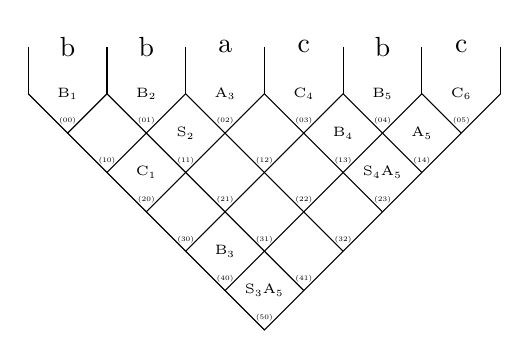
\begin{tikzpicture}[baseline]
			\newcommand{\myfontvars}[1]{
				\fontsize{4.9}{12}\selectfont{#1}
			}\newcommand{\myfontnumbering}[1]{
				\fontsize{2.5}{12}\selectfont{#1}
			}%Outer hull
			%Tip of the pyramid
			\coordinate (tip) at (3.0,-3.0);
			\foreach \i in {0,...,6} {
				\coordinate (\i) at (\i,0);
			}
			%Draw the left and right line of the pyramid pointing downwards
			\draw (0) -- (tip) -- (6);
			%Grid lines direction down-left to top-right
			\coordinate (dl1) at (0.5,-0.5);
			\coordinate (dl2) at (1.0,-1.0);
			\coordinate (dl3) at (1.5,-1.5);
			\coordinate (dl4) at (2.0,-2.0);
			\coordinate (dl5) at (2.5,-2.5);
			\draw (dl1) -- (1,0);
			\draw (dl2) -- (2,0);
			\draw (dl3) -- (3,0);
			\draw (dl4) -- (4,0);
			\draw (dl5) -- (5,0);
			%Grid lines direction down-right to top-left
			\coordinate (dr1) at (3.5,-2.5);
			\coordinate (dr2) at (4.0,-2.0);
			\coordinate (dr3) at (4.5,-1.5);
			\coordinate (dr4) at (5.0,-1.0);
			\coordinate (dr5) at (5.5,-0.5);
			\draw (dr1) -- (1,0);
			\draw (dr2) -- (2,0);
			\draw (dr3) -- (3,0);
			\draw (dr4) -- (4,0);
			\draw (dr5) -- (5,0);
			%Small lines at the top
			\coordinate (top0) at (0.0,0.0);
			\coordinate (top1) at (1.0,0.0);
			\coordinate (top2) at (2.0,0.0);
			\coordinate (top3) at (3.0,0.0);
			\coordinate (top4) at (4.0,0.0);
			\coordinate (top5) at (5.0,0.0);
			\coordinate (top6) at (6.0,0.0);
			\coordinate (topUpper0) at (0.0,0.6);
			\coordinate (topUpper1) at (1.0,0.6);
			\coordinate (topUpper2) at (2.0,0.6);
			\coordinate (topUpper3) at (3.0,0.6);
			\coordinate (topUpper4) at (4.0,0.6);
			\coordinate (topUpper5) at (5.0,0.6);
			\coordinate (topUpper6) at (6.0,0.6);
			\draw (top0) -- (topUpper0);
			\draw (top1) -- (topUpper1);
			\draw (top2) -- (topUpper2);
			\draw (top3) -- (topUpper3);
			\draw (top4) -- (topUpper4);
			\draw (top5) -- (topUpper5);
			\draw (top6) -- (topUpper6);
			%The string
			\coordinate (w0) at (0.5,0.6);
			\coordinate (w1) at (1.5,0.6);
			\coordinate (w2) at (2.5,0.6);
			\coordinate (w3) at (3.5,0.6);
			\coordinate (w4) at (4.5,0.6);
			\coordinate (w5) at (5.5,0.6);
			\node [] at (w0) {b};
			\node [] at (w1) {b};
			\node [] at (w2) {a};
			\node [] at (w3) {c};
			\node [] at (w4) {b};
			\node [] at (w5) {c};
			% Variables in the cells
			%cells00
			\coordinate (center00) at (0.5,0.0);
			\node [below=0.18cm] at (center00) {\myfontnumbering{$(00)$}};
			\node [] at (center00) {\myfontvars{B$_{1}$}};
			%cells01
			\coordinate (center01) at (1.5,0.0);
			\node [below=0.18cm] at (center01) {\myfontnumbering{$(01)$}};
			\node [] at (center01) {\myfontvars{B$_{2}$}};
			%cells02
			\coordinate (center02) at (2.5,0.0);
			\node [below=0.18cm] at (center02) {\myfontnumbering{$(02)$}};
			\node [] at (center02) {\myfontvars{A$_{3}$}};
			%cells03
			\coordinate (center03) at (3.5,0.0);
			\node [below=0.18cm] at (center03) {\myfontnumbering{$(03)$}};
			\node [] at (center03) {\myfontvars{C$_{4}$}};
			%cells04
			\coordinate (center04) at (4.5,0.0);
			\node [below=0.18cm] at (center04) {\myfontnumbering{$(04)$}};
			\node [] at (center04) {\myfontvars{B$_{5}$}};
			%cells05
			\coordinate (center05) at (5.5,0.0);
			\node [below=0.18cm] at (center05) {\myfontnumbering{$(05)$}};
			\node [] at (center05) {\myfontvars{C$_{6}$}};
			%cells10
			\coordinate (center10) at (1.0,-0.5);
			\node [below=0.18cm] at (center10) {\myfontnumbering{$(10)$}};
			%cells11
			\coordinate (center11) at (2.0,-0.5);
			\node [below=0.18cm] at (center11) {\myfontnumbering{$(11)$}};
			\node [] at (center11) {\myfontvars{S$_{2}$}};
			%cells12
			\coordinate (center12) at (3.0,-0.5);
			\node [below=0.18cm] at (center12) {\myfontnumbering{$(12)$}};
			%cells13
			\coordinate (center13) at (4.0,-0.5);
			\node [below=0.18cm] at (center13) {\myfontnumbering{$(13)$}};
			\node [] at (center13) {\myfontvars{B$_{4}$}};
			%cells14
			\coordinate (center14) at (5.0,-0.5);
			\node [below=0.18cm] at (center14) {\myfontnumbering{$(14)$}};
			\node [] at (center14) {\myfontvars{A$_{5}$}};
			%cells20
			\coordinate (center20) at (1.5,-1.0);
			\node [below=0.18cm] at (center20) {\myfontnumbering{$(20)$}};
			\node [] at (center20) {\myfontvars{C$_{1}$}};
			%cells21
			\coordinate (center21) at (2.5,-1.0);
			\node [below=0.18cm] at (center21) {\myfontnumbering{$(21)$}};
			%cells22
			\coordinate (center22) at (3.5,-1.0);
			\node [below=0.18cm] at (center22) {\myfontnumbering{$(22)$}};
			%cells23
			\coordinate (center23) at (4.5,-1.0);
			\node [below=0.18cm] at (center23) {\myfontnumbering{$(23)$}};
			\node [] at (center23) {\myfontvars{S$_{4}$A$_{5}$}};
			%cells30
			\coordinate (center30) at (2.0,-1.5);
			\node [below=0.18cm] at (center30) {\myfontnumbering{$(30)$}};
			%cells31
			\coordinate (center31) at (3.0,-1.5);
			\node [below=0.18cm] at (center31) {\myfontnumbering{$(31)$}};
			%cells32
			\coordinate (center32) at (4.0,-1.5);
			\node [below=0.18cm] at (center32) {\myfontnumbering{$(32)$}};
			%cells40
			\coordinate (center40) at (2.5,-2.0);
			\node [below=0.18cm] at (center40) {\myfontnumbering{$(40)$}};
			\node [] at (center40) {\myfontvars{B$_{3}$}};
			%cells41
			\coordinate (center41) at (3.5,-2.0);
			\node [below=0.18cm] at (center41) {\myfontnumbering{$(41)$}};
			%cells50
			\coordinate (center50) at (3.0,-2.5);
			\node [below=0.18cm] at (center50) {\myfontnumbering{$(50)$}};
			\node [] at (center50) {\myfontvars{S$_{3}$A$_{5}$}};
			\end{tikzpicture}
		}
	\end{minipage}
	\captionof{figure}{Illustration of Algorithm \ref{SplitAndFill} part 6. Comparison of the last step of the algorithm and the complete parsing table.}
	\label{IllustrationAlgorithmSplitAndFillPart6}
	
\end{testexample}






\noindent
\begin{figure} [h]
	
\end{figure}

\clearpage
\pagebreak
\subsection{Evaluation of Algorithms} \label{AnalysisOfAlgorithms}
\subsubsection{Success Rates} \label{successRates}
\noindent Until now different algorithms have been described that could be used in the application to create suitable exam $exercises$. But it is of interest to find out which algorithm performs the best and which algorithm should actually be used in the application to generate the $exercise$s. Therefore a composite $Success~Rate$ is defined that measures the algorithms performance for the different requirements towards an exam $exercise$.  \\

\noindent Here $N \in  \mathbb{N}$ is the sample size of all generated grammars while examining the algorithms. Before defining the overall Success Rate ($SR$) three other Success Rates set the basis for it.\\

\noindent\textbf{Success Rate Producibility: }
A generated $exercise$ contributes to the SR-Producibility if the CYK algorithm's output (Algorithm \ref{CYK}) is true or in other words $w\in L(G)$.\\
SR-Producibility $ = p / N$, where $p$ is the count of $exercise$s that fulfil the requirement.\\

\noindent\textbf{Success Rate Cardinality-Rules: }
A generated $exercise$ contributes to the SR-Cardinality-Rules if the grammar has less than a certain count $x$ of rules, i.e. $|P|\leq x$ of the grammar $G=(V,\ \Sigma,\ S,\ P)$.\\
SR-Cardinality-Rules $ = cr / N$, where $cr$ is the count of $exercise$s that fulfil the requirement.\\

\noindent\textbf{Success Rate Pyramid: }
A generated $exercise$ contributes to the SR-Pyramid if the following conditions are met:
\begin{enumerate} [noitemsep]
	\item At least one cell enforces to a correct cell combination \textendash~see the description of Algorithm \ref{checkForceCombinationPerCell} CheckforceCombinationPerCell for more information.
	\item There are less than 100 variables in the entire pyramid.
	\item There are less than 3 variables in each cell of the pyramid.
\end{enumerate}
SR-Pyramid $= p / N$, where $p$ is the count of $exercise$s that fulfil the three requirements above. \\

\noindent For the sake of these checks (1., 2. and 3.) the definition of a $cell$ in the $pyramid$ is simplified as following:\\ 
$Cell_{i,j} \subseteq \{(V,k)~|~k \in \mathbb{N} \} \longrightarrow Cell_{i,j} \subseteq V$\\
For further illustration see Figure \ref{simplificationExample} on the next page. 
\clearpage

\begin{testexample}[Simplification of cell in a pyramid]
	\noindent The pyramid with the simpler cells is shown right.\\
	
	\begin{minipage}{6in}
		\centering
		\centering
		\raisebox{-0.5\height}{
			\resizebox{0.45\linewidth}{!}{
				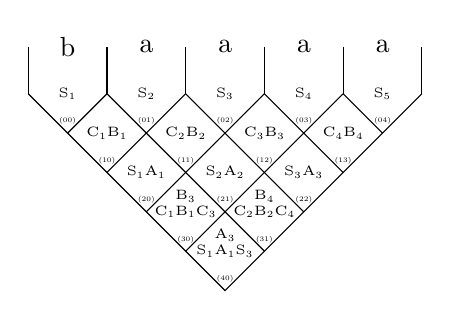
\begin{tikzpicture}[baseline]
				\newcommand{\myfontvars}[1]{
					\fontsize{4.9}{12}\selectfont{#1}
				}\newcommand{\myfontnumbering}[1]{
					\fontsize{2.5}{12}\selectfont{#1}
				}%Outer hull
				%Tip of the pyramid
				\coordinate (tip) at (2.5,-2.5);
				\foreach \i in {0,...,5} {
					\coordinate (\i) at (\i,0);
				}
				%Draw the left and right line of the pyramid pointing downwards
				\draw (0) -- (tip) -- (5);
				%Grid lines direction down-left to top-right
				\coordinate (dl1) at (0.5,-0.5);
				\coordinate (dl2) at (1.0,-1.0);
				\coordinate (dl3) at (1.5,-1.5);
				\coordinate (dl4) at (2.0,-2.0);
				\draw (dl1) -- (1,0);
				\draw (dl2) -- (2,0);
				\draw (dl3) -- (3,0);
				\draw (dl4) -- (4,0);
				%Grid lines direction down-right to top-left
				\coordinate (dr1) at (3.0,-2.0);
				\coordinate (dr2) at (3.5,-1.5);
				\coordinate (dr3) at (4.0,-1.0);
				\coordinate (dr4) at (4.5,-0.5);
				\draw (dr1) -- (1,0);
				\draw (dr2) -- (2,0);
				\draw (dr3) -- (3,0);
				\draw (dr4) -- (4,0);
				%Small lines at the top
				\coordinate (top0) at (0.0,0.0);
				\coordinate (top1) at (1.0,0.0);
				\coordinate (top2) at (2.0,0.0);
				\coordinate (top3) at (3.0,0.0);
				\coordinate (top4) at (4.0,0.0);
				\coordinate (top5) at (5.0,0.0);
				\coordinate (topUpper0) at (0.0,0.6);
				\coordinate (topUpper1) at (1.0,0.6);
				\coordinate (topUpper2) at (2.0,0.6);
				\coordinate (topUpper3) at (3.0,0.6);
				\coordinate (topUpper4) at (4.0,0.6);
				\coordinate (topUpper5) at (5.0,0.6);
				\draw (top0) -- (topUpper0);
				\draw (top1) -- (topUpper1);
				\draw (top2) -- (topUpper2);
				\draw (top3) -- (topUpper3);
				\draw (top4) -- (topUpper4);
				\draw (top5) -- (topUpper5);
				%The string
				\coordinate (w0) at (0.5,0.6);
				\coordinate (w1) at (1.5,0.6);
				\coordinate (w2) at (2.5,0.6);
				\coordinate (w3) at (3.5,0.6);
				\coordinate (w4) at (4.5,0.6);
				\node [] at (w0) {b};
				\node [] at (w1) {a};
				\node [] at (w2) {a};
				\node [] at (w3) {a};
				\node [] at (w4) {a};
				% Variables in the cells
				%cells00
				\coordinate (center00) at (0.5,0.0);
				\node [below=0.18cm] at (center00) {\myfontnumbering{$(00)$}};
				\node [] at (center00) {\myfontvars{S$_{1}$}};
				%cells01
				\coordinate (center01) at (1.5,0.0);
				\node [below=0.18cm] at (center01) {\myfontnumbering{$(01)$}};
				\node [] at (center01) {\myfontvars{S$_{2}$}};
				%cells02
				\coordinate (center02) at (2.5,0.0);
				\node [below=0.18cm] at (center02) {\myfontnumbering{$(02)$}};
				\node [] at (center02) {\myfontvars{S$_{3}$}};
				%cells03
				\coordinate (center03) at (3.5,0.0);
				\node [below=0.18cm] at (center03) {\myfontnumbering{$(03)$}};
				\node [] at (center03) {\myfontvars{S$_{4}$}};
				%cells04
				\coordinate (center04) at (4.5,0.0);
				\node [below=0.18cm] at (center04) {\myfontnumbering{$(04)$}};
				\node [] at (center04) {\myfontvars{S$_{5}$}};
				%cells10
				\coordinate (center10) at (1.0,-0.5);
				\node [below=0.18cm] at (center10) {\myfontnumbering{$(10)$}};
				\node [] at (center10) {\myfontvars{C$_{1}$B$_{1}$}};
				%cells11
				\coordinate (center11) at (2.0,-0.5);
				\node [below=0.18cm] at (center11) {\myfontnumbering{$(11)$}};
				\node [] at (center11) {\myfontvars{C$_{2}$B$_{2}$}};
				%cells12
				\coordinate (center12) at (3.0,-0.5);
				\node [below=0.18cm] at (center12) {\myfontnumbering{$(12)$}};
				\node [] at (center12) {\myfontvars{C$_{3}$B$_{3}$}};
				%cells13
				\coordinate (center13) at (4.0,-0.5);
				\node [below=0.18cm] at (center13) {\myfontnumbering{$(13)$}};
				\node [] at (center13) {\myfontvars{C$_{4}$B$_{4}$}};
				%cells20
				\coordinate (center20) at (1.5,-1.0);
				\node [below=0.18cm] at (center20) {\myfontnumbering{$(20)$}};
				\node [] at (center20) {\myfontvars{S$_{1}$A$_{1}$}};
				%cells21
				\coordinate (center21) at (2.5,-1.0);
				\node [below=0.18cm] at (center21) {\myfontnumbering{$(21)$}};
				\node [] at (center21) {\myfontvars{S$_{2}$A$_{2}$}};
				%cells22
				\coordinate (center22) at (3.5,-1.0);
				\node [below=0.18cm] at (center22) {\myfontnumbering{$(22)$}};
				\node [] at (center22) {\myfontvars{S$_{3}$A$_{3}$}};
				%cells30
				\coordinate (center30) at (2.0,-1.5);
				\node [below=0.18cm] at (center30) {\myfontnumbering{$(30)$}};
				\node [] at (center30) {\myfontvars{C$_{1}$B$_{1}$C$_{3}$}};
				\node [above] at (center30) {\myfontvars{B$_{3}$}};
				%cells31
				\coordinate (center31) at (3.0,-1.5);
				\node [below=0.18cm] at (center31) {\myfontnumbering{$(31)$}};
				\node [] at (center31) {\myfontvars{C$_{2}$B$_{2}$C$_{4}$}};
				\node [above] at (center31) {\myfontvars{B$_{4}$}};
				%cells40
				\coordinate (center40) at (2.5,-2.0);
				\node [below=0.18cm] at (center40) {\myfontnumbering{$(40)$}};
				\node [] at (center40) {\myfontvars{S$_{1}$A$_{1}$S$_{3}$}};
				\node [above] at (center40) {\myfontvars{A$_{3}$}};
				\end{tikzpicture}
			}
		}
		\hspace*{.2in}
		\raisebox{-0.5\height}{
			\resizebox{0.45\linewidth}{!}{
				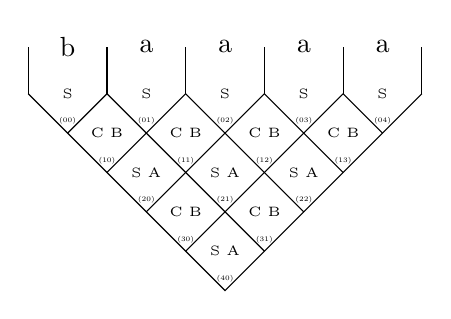
\begin{tikzpicture}[baseline]
				\newcommand{\myfontvars}[1]{
					\fontsize{4.9}{12}\selectfont{#1}
				}\newcommand{\myfontnumbering}[1]{
					\fontsize{2.5}{12}\selectfont{#1}
				}%Outer hull
				%Tip of the pyramid
				\coordinate (tip) at (2.5,-2.5);
				\foreach \i in {0,...,5} {
					\coordinate (\i) at (\i,0);
				}
				%Draw the left and right line of the pyramid pointing downwards
				\draw (0) -- (tip) -- (5);
				%Grid lines direction down-left to top-right
				\coordinate (dl1) at (0.5,-0.5);
				\coordinate (dl2) at (1.0,-1.0);
				\coordinate (dl3) at (1.5,-1.5);
				\coordinate (dl4) at (2.0,-2.0);
				\draw (dl1) -- (1,0);
				\draw (dl2) -- (2,0);
				\draw (dl3) -- (3,0);
				\draw (dl4) -- (4,0);
				%Grid lines direction down-right to top-left
				\coordinate (dr1) at (3.0,-2.0);
				\coordinate (dr2) at (3.5,-1.5);
				\coordinate (dr3) at (4.0,-1.0);
				\coordinate (dr4) at (4.5,-0.5);
				\draw (dr1) -- (1,0);
				\draw (dr2) -- (2,0);
				\draw (dr3) -- (3,0);
				\draw (dr4) -- (4,0);
				%Small lines at the top
				\coordinate (top0) at (0.0,0.0);
				\coordinate (top1) at (1.0,0.0);
				\coordinate (top2) at (2.0,0.0);
				\coordinate (top3) at (3.0,0.0);
				\coordinate (top4) at (4.0,0.0);
				\coordinate (top5) at (5.0,0.0);
				\coordinate (topUpper0) at (0.0,0.6);
				\coordinate (topUpper1) at (1.0,0.6);
				\coordinate (topUpper2) at (2.0,0.6);
				\coordinate (topUpper3) at (3.0,0.6);
				\coordinate (topUpper4) at (4.0,0.6);
				\coordinate (topUpper5) at (5.0,0.6);
				\draw (top0) -- (topUpper0);
				\draw (top1) -- (topUpper1);
				\draw (top2) -- (topUpper2);
				\draw (top3) -- (topUpper3);
				\draw (top4) -- (topUpper4);
				\draw (top5) -- (topUpper5);
				%The string
				\coordinate (w0) at (0.5,0.6);
				\coordinate (w1) at (1.5,0.6);
				\coordinate (w2) at (2.5,0.6);
				\coordinate (w3) at (3.5,0.6);
				\coordinate (w4) at (4.5,0.6);
				\node [] at (w0) {b};
				\node [] at (w1) {a};
				\node [] at (w2) {a};
				\node [] at (w3) {a};
				\node [] at (w4) {a};
				% Variables in the cells
				%cells00
				\coordinate (center00) at (0.5,0.0);
				\node [below=0.18cm] at (center00) {\myfontnumbering{$(00)$}};
				\node [] at (center00) {\myfontvars{S}};
				%cells01
				\coordinate (center01) at (1.5,0.0);
				\node [below=0.18cm] at (center01) {\myfontnumbering{$(01)$}};
				\node [] at (center01) {\myfontvars{S}};
				%cells02
				\coordinate (center02) at (2.5,0.0);
				\node [below=0.18cm] at (center02) {\myfontnumbering{$(02)$}};
				\node [] at (center02) {\myfontvars{S}};
				%cells03
				\coordinate (center03) at (3.5,0.0);
				\node [below=0.18cm] at (center03) {\myfontnumbering{$(03)$}};
				\node [] at (center03) {\myfontvars{S}};
				%cells04
				\coordinate (center04) at (4.5,0.0);
				\node [below=0.18cm] at (center04) {\myfontnumbering{$(04)$}};
				\node [] at (center04) {\myfontvars{S}};
				%cells10
				\coordinate (center10) at (1.0,-0.5);
				\node [below=0.18cm] at (center10) {\myfontnumbering{$(10)$}};
				\node [] at (center10) {\myfontvars{C B}};
				%cells11
				\coordinate (center11) at (2.0,-0.5);
				\node [below=0.18cm] at (center11) {\myfontnumbering{$(11)$}};
				\node [] at (center11) {\myfontvars{C B}};
				%cells12
				\coordinate (center12) at (3.0,-0.5);
				\node [below=0.18cm] at (center12) {\myfontnumbering{$(12)$}};
				\node [] at (center12) {\myfontvars{C B}};
				%cells13
				\coordinate (center13) at (4.0,-0.5);
				\node [below=0.18cm] at (center13) {\myfontnumbering{$(13)$}};
				\node [] at (center13) {\myfontvars{C B}};
				%cells20
				\coordinate (center20) at (1.5,-1.0);
				\node [below=0.18cm] at (center20) {\myfontnumbering{$(20)$}};
				\node [] at (center20) {\myfontvars{S A}};
				%cells21
				\coordinate (center21) at (2.5,-1.0);
				\node [below=0.18cm] at (center21) {\myfontnumbering{$(21)$}};
				\node [] at (center21) {\myfontvars{S A}};
				%cells22
				\coordinate (center22) at (3.5,-1.0);
				\node [below=0.18cm] at (center22) {\myfontnumbering{$(22)$}};
				\node [] at (center22) {\myfontvars{S A}};
				%cells30
				\coordinate (center30) at (2.0,-1.5);
				\node [below=0.18cm] at (center30) {\myfontnumbering{$(30)$}};
				\node [] at (center30) {\myfontvars{C B}};
				%cells31
				\coordinate (center31) at (3.0,-1.5);
				\node [below=0.18cm] at (center31) {\myfontnumbering{$(31)$}};
				\node [] at (center31) {\myfontvars{C B}};
				%cells40
				\coordinate (center40) at (2.5,-2.0);
				\node [below=0.18cm] at (center40) {\myfontnumbering{$(40)$}};
				\node [] at (center40) {\myfontvars{S A}};
				\end{tikzpicture}
			}
		}
	\end{minipage}
	\captionof{figure}{The simplification of cells in a pyramid.}
	\label{simplificationExample}
\end{testexample}

\noindent \textbf{Description of the Algorithm CheckForceCombinationPerCell: }\\
The experience of professor Martens shows that usually most students easily find a pattern of how to fill the first two rows of the $pyramid$ during the execution of the CYK algorithm but do more mistakes starting at row $i\geq2$. Students often do not know exactly what cell combinations need to be considered while filling one specific cell of the pyramid. They simply take only the one top left cell and the one top right cell and try to find rules in the grammar that match the resulting compound variables. The approach of only finding patterns and not thoroughly understanding the algorithm is countered by Algorithm \ref{checkForceCombinationPerCell} CheckForceCombinationPerCell. Here a cell forces if it is possible to see if the student has clearly understood the algorithm and not only takes the next top left cell and the next top right cell.\\

\noindent 
\frame{
	\begin{algorithm}[H] %or another one check
		\caption{CheckForceCombinationPerCell}
		\label{checkForceCombinationPerCell}
		\SetAlgoLined
		\KwIn{$ CellBottom,~CellTopLeft,~CellTopRight \subseteq V,~P \subseteq V \times (V^{2} \cup \Sigma) $ }
		\KwOut{$true \iff |VarsForcing| > 0$}
		$VarsForcing = \emptyset$;~~\tcp{$VarsForcing \subseteq V$} 
		$VarComp = \{xy\ |\ x \in CellTopLeft\ \wedge\ y \in CellTopRight \}$\;
		\ForEach{$v \in CellDown$}{
			$Rhses = \{rhse\ |\ p \in P\ \wedge\ p=(v,rhse)\} $\; \label{rhses}
			\If{$Rhses \nsubseteq VarComp$}{ \label{forces}
				$VarsForcing = VarsForcing \cup v$\;
			}			
		}
		\Return $|VarsForcing| > 0$\;
		\footnotetext{
			Note: $CellBottom=Cell_{i,j}$, $CellTopLeft=Cell_{i-1,j}$ and  $CellTopRight=Cell_{i-1,j-1}$\\
			Line \ref{rhses}: Get all rules of $P$ that have $v$ as the $lhse$ and add their $rhse$ to $Rhses$.\\
			Line \ref{forces}: If no $rhse \in Rhse$ can be found in VarComp, then this variables forces, concluding that this cell as a hole forces.
		}
	\end{algorithm}
}

\begin{testexample}[Algorithm CheckForceCombinationPerCell]
	\noindent In Figure \ref{foreCombination}, the variables in $Cell_{2,0}$ and in $Cell_{2,1}$ each force a right cell combination and in both cases $VarComp=\{SS\}$. The variable $v=C$ does not have $SS$ as one of its rhses and therefore the variable $C$ forces. $Cell_{3,0}$ does not force because $VarComp=\{CC\}$ and the variable $v=S$ has $CC$ as its rhse. Note again, that cells with index $i\leq1$ can not force at all.\\
	
	\begin{minipage}{6in}
		\centering
			\centering
		\raisebox{-0.5\height}{
			\begin{tabular}{l}
				$Grammar:$\\
				$C\rightarrow C S~|~a~|~b$\\ 
				$S\rightarrow C C~~$\\ 
			\end{tabular} 
		}
		\hspace*{.2in}
		\raisebox{-0.5\height}{
			\resizebox{0.5\linewidth}{!}{
				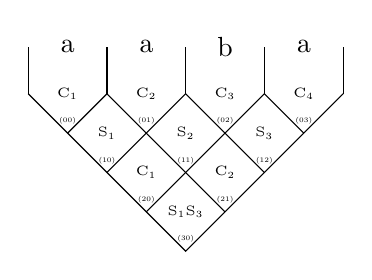
\begin{tikzpicture}[baseline]
				\newcommand{\myfontvars}[1]{
					\fontsize{4.9}{12}\selectfont{#1}
				}\newcommand{\myfontnumbering}[1]{
					\fontsize{2.5}{12}\selectfont{#1}
				}%Outer hull
				%Tip of the pyramid
				\coordinate (tip) at (2.0,-2.0);
				\foreach \i in {0,...,4} {
					\coordinate (\i) at (\i,0);
				}
				%Draw the left and right line of the pyramid pointing downwards
				\draw (0) -- (tip) -- (4);
				%Grid lines direction down-left to top-right
				\coordinate (dl1) at (0.5,-0.5);
				\coordinate (dl2) at (1.0,-1.0);
				\coordinate (dl3) at (1.5,-1.5);
				\draw (dl1) -- (1,0);
				\draw (dl2) -- (2,0);
				\draw (dl3) -- (3,0);
				%Grid lines direction down-right to top-left
				\coordinate (dr1) at (2.5,-1.5);
				\coordinate (dr2) at (3.0,-1.0);
				\coordinate (dr3) at (3.5,-0.5);
				\draw (dr1) -- (1,0);
				\draw (dr2) -- (2,0);
				\draw (dr3) -- (3,0);
				%Small lines at the top
				\coordinate (top0) at (0.0,0.0);
				\coordinate (top1) at (1.0,0.0);
				\coordinate (top2) at (2.0,0.0);
				\coordinate (top3) at (3.0,0.0);
				\coordinate (top4) at (4.0,0.0);
				\coordinate (topUpper0) at (0.0,0.6);
				\coordinate (topUpper1) at (1.0,0.6);
				\coordinate (topUpper2) at (2.0,0.6);
				\coordinate (topUpper3) at (3.0,0.6);
				\coordinate (topUpper4) at (4.0,0.6);
				\draw (top0) -- (topUpper0);
				\draw (top1) -- (topUpper1);
				\draw (top2) -- (topUpper2);
				\draw (top3) -- (topUpper3);
				\draw (top4) -- (topUpper4);
				%The string
				\coordinate (w0) at (0.5,0.6);
				\coordinate (w1) at (1.5,0.6);
				\coordinate (w2) at (2.5,0.6);
				\coordinate (w3) at (3.5,0.6);
				\node [] at (w0) {a};
				\node [] at (w1) {a};
				\node [] at (w2) {b};
				\node [] at (w3) {a};
				% Variables in the cells
				%cells00
				\coordinate (center00) at (0.5,0.0);
				\node [below=0.18cm] at (center00) {\myfontnumbering{$(00)$}};
				\node [] at (center00) {\myfontvars{C$_{1}$}};
				%cells01
				\coordinate (center01) at (1.5,0.0);
				\node [below=0.18cm] at (center01) {\myfontnumbering{$(01)$}};
				\node [] at (center01) {\myfontvars{C$_{2}$}};
				%cells02
				\coordinate (center02) at (2.5,0.0);
				\node [below=0.18cm] at (center02) {\myfontnumbering{$(02)$}};
				\node [] at (center02) {\myfontvars{C$_{3}$}};
				%cells03
				\coordinate (center03) at (3.5,0.0);
				\node [below=0.18cm] at (center03) {\myfontnumbering{$(03)$}};
				\node [] at (center03) {\myfontvars{C$_{4}$}};
				%cells10
				\coordinate (center10) at (1.0,-0.5);
				\node [below=0.18cm] at (center10) {\myfontnumbering{$(10)$}};
				\node [] at (center10) {\myfontvars{S$_{1}$}};
				%cells11
				\coordinate (center11) at (2.0,-0.5);
				\node [below=0.18cm] at (center11) {\myfontnumbering{$(11)$}};
				\node [] at (center11) {\myfontvars{S$_{2}$}};
				%cells12
				\coordinate (center12) at (3.0,-0.5);
				\node [below=0.18cm] at (center12) {\myfontnumbering{$(12)$}};
				\node [] at (center12) {\myfontvars{S$_{3}$}};
				%cells20
				\coordinate (center20) at (1.5,-1.0);
				\node [below=0.18cm] at (center20) {\myfontnumbering{$(20)$}};
				\node [] at (center20) {\myfontvars{C$_{1}$}};
				%cells21
				\coordinate (center21) at (2.5,-1.0);
				\node [below=0.18cm] at (center21) {\myfontnumbering{$(21)$}};
				\node [] at (center21) {\myfontvars{C$_{2}$}};
				%cells30
				\coordinate (center30) at (2.0,-1.5);
				\node [below=0.18cm] at (center30) {\myfontnumbering{$(30)$}};
				\node [] at (center30) {\myfontvars{S$_{1}$S$_{3}$}};
				\end{tikzpicture}
			}
		}
	\end{minipage}
	\captionof{figure}{Application of Algorithm \ref{checkForceCombinationPerCell} CheckForceCombinationPerCell onto an entire pyramid.}
	\label{foreCombination}
\end{testexample}

\noindent The three success rates have been explained and finally the overall Success Rate can be specified. \\
\noindent\textbf{Success Rate:}
A generated $exercise$ contributes to the Success Rate (SR) if it contributes to the SR-Producibility, to the SR-Cardinality-Rules and to the SR-Pyramid at the same time.\\
It holds: $SR = n / N$, where $n$ is the count of $exercises$.
\subsubsection{Problem space exploration}
Suitable ranges of parameters, to create exam $exercises$ with, are:
\begin{itemize}[noitemsep,nolistsep]
	\item count of variables = [2;~8]
	\item count of terminals = [2;~8]
	\item size of word = [4;~11]
\end{itemize}
%\vspace{0.6cm}
This input parameter ranges are used during further comparison. Each calculated SR is based on a batch size N = 1024.
\clearpage
\paragraph{Comparison of the stopping criteria}~\\
As described in Chapter \ref{subModules} Sub Modules, two different stopping criteria \circled{C} are used and it is of interest to know which one helps to generate more suitable exam $exercise$s so that the better one can be used in a real world application. Therefore both variants of the stopping criteria are compared in Table \ref{comparisionMeanValue} and Table \ref{comparisionStoppingCriteria}.\\
Table \ref{comparisionMeanValue} shows the average SRs over all configurations of parameters for each algorithm.

\begin{table}[h]
	\centering
	\begin{tabular}{l|c|c|}
		\cline{2-3}
		& MoreThanHalf & RootNotEmpty \\ \hline
		\multicolumn{1}{|l|}{DiceRollOnly}  & 0.3\%             & \textbf{0.3\%}            \\ \hline
		\multicolumn{1}{|l|}{DiceRollVar1}  & 0.5\%             & \textbf{1.3\%}            \\ \hline
		\multicolumn{1}{|l|}{DiceRollVar2}  & 0.6\%             & \textbf{1.7\%}            \\ \hline
		\multicolumn{1}{|l|}{SplitThenFill} & 1.4\%             & \textbf{1.4\%}            \\ \hline
		\multicolumn{1}{|l|}{SplitAndFill}  & 8.4\%             & \textbf{8.4\%}             \\ \hline
	\end{tabular}
	\caption{Average SRs over all the configurations of parameters for each algorithm.}
	\label{comparisionMeanValue}
\end{table}

\noindent In Table \ref{comparisionStoppingCriteria} the best possible SRs of each algorithm are compared.\\



\begin{table}[h]
	\centering
		\begin{tabular}{l|c|c|}
			\cline{2-3}
			& MoreThanHalf & RootNotEmpty \\ \hline
			\multicolumn{1}{|l|}{DiceRollOnly}  & 17\%             & \textbf{17\%}            \\ \hline
			\multicolumn{1}{|l|}{DiceRollVar1}  & 18\%             & \textbf{36\%}            \\ \hline
			\multicolumn{1}{|l|}{DiceRollVar2}  & 20\%             & \textbf{38\%}            \\ \hline
			\multicolumn{1}{|l|}{SplitThenFill} & 36\%             & \textbf{36\%}            \\ \hline
			\multicolumn{1}{|l|}{SplitAndFill}  & 74\%             & \textbf{74\%}             \\ \hline
		\end{tabular}
	\caption{Comparison of the best possible SRs of each algorithm. (N = 1024)}
	\label{comparisionStoppingCriteria}
\end{table}
\noindent As seen in the two tables above (Table \ref{comparisionMeanValue} and Table \ref{comparisionStoppingCriteria}), the stopping criteria RootNotEmpty performs better or at least equally good in every case. RootNotEmpty wins through and all further discussion in the following Chapter \ref{comparisonOfTheAlgorithms} is done with it.
\clearpage
\paragraph{Picking the best algorithm}\label{comparisonOfTheAlgorithms}~\\
Now that the choice of the stopping criteria has been decided in favour of RootNotEmpty it is time to determine the one best algorithm.\\

\noindent As seen in Table \ref{comparisionsAlgorithmsMean} the Algorithm \ref{SplitAndFill} SplitAndFill performs the best in all three sub success rates Producibility, Cardinality-Rules and Pyramid and therefore the algorithm also has the best average overall SR.\\

\begin{table}[h]
	\centering
	\begin{tabular}{|l|c|c|c|c|c|c|c|}
		\hline
		\multicolumn{1}{|c|}{Algorithm} & SR   & \begin{tabular}[c]{@{}c@{}}Produci-\\ bility\end{tabular} & \begin{tabular}[c]{@{}c@{}}Cardinality-\\ Rules\end{tabular} & \multicolumn{4}{c|}{Pyramid}                                                                                                                                                        \\ \cline{6-8} 
		&      &                                                           &                                                              &      & \begin{tabular}[c]{@{}c@{}}Force-\\ Right\end{tabular} & \begin{tabular}[c]{@{}c@{}}Vars-\\ PerCell\end{tabular} & \begin{tabular}[c]{@{}c@{}}VarsIn-\\ Pyramid\end{tabular} \\ \hline
		DiceRollOnly                    & \textbf{0.3\%} & 5.2\%                                                           &2.9\%                                                              & 12.1\% &15.9\%                                                        &24.9\%                                                         &28.4\%                                                           \\ \hline
		BottomUpVar1                    &\textbf{1.3\%}      &7.7\%                                                           &13.5\%                                                              &11.9\%      &19.8\%                                                        &20.8\%                                                         &26.1\%                                                           \\ \hline
		BottomUpVar2                    &\textbf{1.7\%}      &10.9\%                                                           &8.7\%                                                              &13.5\%      &25.4\%                                                        &16.6\%                                                         &25.9\%                                                           \\ \hline
		SplitThenFill                   &\textbf{1.4\%}    &4.3\%                                                           &14.5\%                                                              &14.7\%      &15.8\%                                                        &27.6\%                                                         &28.5\%                                                           \\ \hline
		SplitAndFill                    &\textbf{8.4\%}      &28.7\%                                                           &17.4\%                                                              &14.8\%      &18.3\%                                                        &25.3\%                                                         &27.3\%                                                           \\ \hline
	\end{tabular}
	\caption{More detailed comparision of the average SRs over all the configurations of parameters for each algorithm.}
	\label{comparisionsAlgorithmsMean}
\end{table}
\noindent While looking at Table \ref{comparisionsAlgorithms}, that displays the best possible SRs, Algorithm \ref{SplitAndFill} SplitAndFill again performs the best.\\
 
\begin{table}[h]
	\centering
	\begin{tabular}{|l|c|c|c|c|c|c|c|}
		\hline
		\multicolumn{1}{|c|}{Algorithm} & SR   & \begin{tabular}[c]{@{}c@{}}Produci-\\ bility\end{tabular} & \begin{tabular}[c]{@{}c@{}}Cardinality-\\ Rules\end{tabular} & \multicolumn{4}{c|}{Pyramid}                                                                                                                                                        \\ \cline{6-8} 
		&      &                                                           &                                                              &      & \begin{tabular}[c]{@{}c@{}}Force-\\ Right\end{tabular} & \begin{tabular}[c]{@{}c@{}}Vars-\\ PerCell\end{tabular} & \begin{tabular}[c]{@{}c@{}}VarsIn-\\ Pyramid\end{tabular} \\ \hline
		DiceRollOnly                    & \textbf{17\%} & 21\%                                                           &98\%                                                              & 47\% &47\%                                                        &100\%                                                         &100\%                                                           \\ \hline
		BottomUpVar1                    &\textbf{36\%}      &60\%                                                           &91\%                                                              &65\%      &69\%                                                        &100\%                                                         &93\%                                                           \\ \hline
		BottomUpVar2                    &\textbf{38\%}      &56\%                                                           &95\%                                                              &69\%      &69\%                                                        &100\%                                                         &100\%                                                           \\ \hline
		SplitThenFill                   &\textbf{36\%}    &51\%                                                           &97\%                                                              &71\%      &71\%                                                        &100\%                                                         &99\%                                                           \\ \hline
		SplitAndFill                    &\textbf{74\%}      &100\%                                                           &100\%                                                              &74\%      &74\%                                                        &100\%                                                         &100\%                                                           \\ \hline
	\end{tabular}
	\caption{More detailed comparison of the best possible SRs of each algorithm. (N = 1024)}
	\label{comparisionsAlgorithms}
\end{table}
\noindent The Algorithm \ref{SplitAndFill} SplitAndFill wins through against the other four as it leads to the best SR on average and also has the best possible SR of all algorithms. \\

\noindent Therefore the Algorithm SplitAndFill is the best choice to use in an application.

\clearpage
\pagebreak
	
	% !TeX spellcheck = en_GB

\section{CLI Tool}
Write much of this stuff in the appendix.

\subsection{Scoring Model}

Only valid ResultSamples are given a score. Parameters to be scored:
\begin{itemize}
	\item RightCellCombinationsForcedCount
	\item maxSumOfVarsInPyramidCount 	
	\item maxNumberOfVarsPerCellCount
	\item maxSumOfProductionsCount
\end{itemize}

\noindent Maybe add a diversity criterion = homogeneity of the cells to the scoring matrix.

\begin{table}[H]
	\centering
	\begin{tabular}{|l|c|c|c|c|c|l|}
		\hline
		\multicolumn{1}{|c|}{\multirow{2}{*}{Parameter}} & \multicolumn{6}{c|}{Points}                                                          \\ \cline{2-7} 
		\multicolumn{1}{|c|}{}                           & 2          & 4           & 6           & 8           & 10          & -100            \\ \hline
		cellCombinationsForced                           & {[}0,10{]} & {[}11,20{]} & {[}21,30{]} & {[}41,50{]} & {[}31,40{]} & \textgreater 50 \\ \hline
		sumVarsInPyramid                                 & {[}0,10{]} & {[}11,20{]} & {[}21,30{]} & {[}41,50{]} & {[}31,40{]} & \textgreater 50 \\ \hline
		maxVarsPerCell                                   & {[}5,5{]}  & {[}4,4{]}   & {[}1,1{]}   & {[}3,3{]}   & {[}2,2{]}   & \textgreater 5  \\ \hline
		sumProductions                                   & {[}1,2{]}  & {[}3,4{]}   & {[}5,6{]}   & {[}9,10{]}  & {[}7,8{]}   & \textgreater 10 \\ \hline
	\end{tabular}
	\caption{Scoring of the different parameter values}
	\label{scoring}
\end{table}



\noindent Based on table \ref{scoring} each result sample is scored. Out of the \#??? best result samples one can choose.\\
The result will be normalized to the maximum possible points -> range 0.0 to 1.0. 

\subsection{Short Requirements Specification}

\noindent Generating the latex code and storing it in .tex-file. Then converting the .tex-file to .pdf-file via:\\
Runtime rt = Runtime.getRuntime();\\
Process pr = rt.exec("pdflatex mydoc.tex");\\
Process pr = rt.exec("pdflatex mydoc.tex");\\
Process pr = rt.exec("pdflatex mydoc.tex");\\
The triple invocation of LaTeX is to ensure that all references have been properly resolved and any page layout changes due to inserting the references have been accounted for. [http://www.arakhne.org/autolatex/]

\subsubsection{Exam Exercises}
4-tuples $exercise = (grammar,\ word,\ parse\ table,\ derivation\ tree)$ that needs to be printed.

\begin{center} 
	\begin{tabular}{l}$A\rightarrow a~|~c~|~BA~~$\\ 
		$B\rightarrow b~|~CB~~$\\ 
		$C\rightarrow c~|~AC~~$\\ 
		$S\rightarrow AB~|~BC~~$\\ 
	\end{tabular} 
\end{center}

\begin{center}
	\resizebox{\linewidth}{!}{
		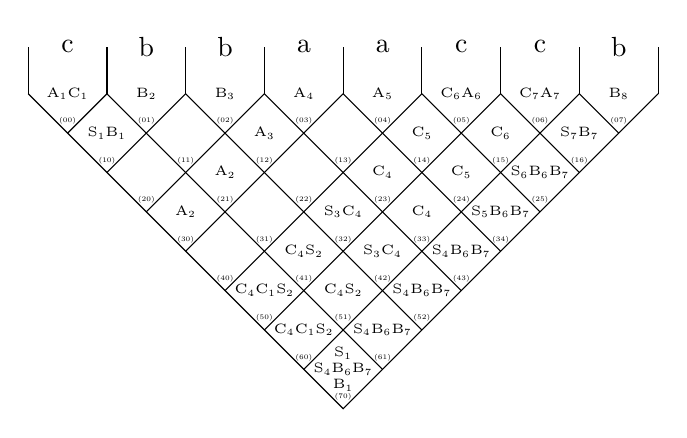
\begin{tikzpicture}[baseline]
		\newcommand{\myfontvars}[1]{
			\fontsize{4.9}{12}\selectfont{#1}
		}\newcommand{\myfontnumbering}[1]{
			\fontsize{2.5}{12}\selectfont{#1}
		}%Outer hull
		%Tip of the pyramid
		\coordinate (tip) at (4,-4);
		\foreach \i in {0,...,8} {
			\coordinate (\i) at (\i,0);
		}
		%Draw the left and right line of the pyramid pointing downwards
		\draw (0) -- (tip) -- (8);
		%Grid lines direction down-left to top-right
		\coordinate (dl1) at (0.5,-0.5);
		\coordinate (dl2) at (1.0,-1.0);
		\coordinate (dl3) at (1.5,-1.5);
		\coordinate (dl4) at (2.0,-2.0);
		\coordinate (dl5) at (2.5,-2.5);
		\coordinate (dl6) at (3.0,-3.0);
		\coordinate (dl7) at (3.5,-3.5);
		\draw (dl1) -- (1,0);
		\draw (dl2) -- (2,0);
		\draw (dl3) -- (3,0);
		\draw (dl4) -- (4,0);
		\draw (dl5) -- (5,0);
		\draw (dl6) -- (6,0);
		\draw (dl7) -- (7,0);
		%Grid lines direction down-right to top-left
		\coordinate (dr1) at (4.5,-3.5);
		\coordinate (dr2) at (5.0,-3.0);
		\coordinate (dr3) at (5.5,-2.5);
		\coordinate (dr4) at (6.0,-2.0);
		\coordinate (dr5) at (6.5,-1.5);
		\coordinate (dr6) at (7.0,-1.0);
		\coordinate (dr7) at (7.5,-0.5);
		\draw (dr1) -- (1,0);
		\draw (dr2) -- (2,0);
		\draw (dr3) -- (3,0);
		\draw (dr4) -- (4,0);
		\draw (dr5) -- (5,0);
		\draw (dr6) -- (6,0);
		\draw (dr7) -- (7,0);
		%Small lines at the top
		\coordinate (top0) at (0.0,0.0);
		\coordinate (top1) at (1.0,0.0);
		\coordinate (top2) at (2.0,0.0);
		\coordinate (top3) at (3.0,0.0);
		\coordinate (top4) at (4.0,0.0);
		\coordinate (top5) at (5.0,0.0);
		\coordinate (top6) at (6.0,0.0);
		\coordinate (top7) at (7.0,0.0);
		\coordinate (top8) at (8.0,0.0);
		\coordinate (topUpper0) at (0.0,0.6);
		\coordinate (topUpper1) at (1.0,0.6);
		\coordinate (topUpper2) at (2.0,0.6);
		\coordinate (topUpper3) at (3.0,0.6);
		\coordinate (topUpper4) at (4.0,0.6);
		\coordinate (topUpper5) at (5.0,0.6);
		\coordinate (topUpper6) at (6.0,0.6);
		\coordinate (topUpper7) at (7.0,0.6);
		\coordinate (topUpper8) at (8.0,0.6);
		\draw (top0) -- (topUpper0);
		\draw (top1) -- (topUpper1);
		\draw (top2) -- (topUpper2);
		\draw (top3) -- (topUpper3);
		\draw (top4) -- (topUpper4);
		\draw (top5) -- (topUpper5);
		\draw (top6) -- (topUpper6);
		\draw (top7) -- (topUpper7);
		\draw (top8) -- (topUpper8);
		%The string
		\coordinate (w0) at (0.5,0.6);
		\coordinate (w1) at (1.5,0.6);
		\coordinate (w2) at (2.5,0.6);
		\coordinate (w3) at (3.5,0.6);
		\coordinate (w4) at (4.5,0.6);
		\coordinate (w5) at (5.5,0.6);
		\coordinate (w6) at (6.5,0.6);
		\coordinate (w7) at (7.5,0.6);
		\node [] at (w0) {c};
		\node [] at (w1) {b};
		\node [] at (w2) {b};
		\node [] at (w3) {a};
		\node [] at (w4) {a};
		\node [] at (w5) {c};
		\node [] at (w6) {c};
		\node [] at (w7) {b};
		% Variables in the cells
		%cells00
		\coordinate (center00) at (0.5,0.0);
		\node [below=0.18cm] at (center00) {\myfontnumbering{$(00)$}};
		\node [] at (center00) {\myfontvars{A$_1$C$_1$}};
		%cells01
		\coordinate (center01) at (1.5,0.0);
		\node [below=0.18cm] at (center01) {\myfontnumbering{$(01)$}};
		\node [] at (center01) {\myfontvars{B$_2$}};
		%cells02
		\coordinate (center02) at (2.5,0.0);
		\node [below=0.18cm] at (center02) {\myfontnumbering{$(02)$}};
		\node [] at (center02) {\myfontvars{B$_3$}};
		%cells03
		\coordinate (center03) at (3.5,0.0);
		\node [below=0.18cm] at (center03) {\myfontnumbering{$(03)$}};
		\node [] at (center03) {\myfontvars{A$_4$}};
		%cells04
		\coordinate (center04) at (4.5,0.0);
		\node [below=0.18cm] at (center04) {\myfontnumbering{$(04)$}};
		\node [] at (center04) {\myfontvars{A$_5$}};
		%cells05
		\coordinate (center05) at (5.5,0.0);
		\node [below=0.18cm] at (center05) {\myfontnumbering{$(05)$}};
		\node [] at (center05) {\myfontvars{C$_6$A$_6$}};
		%cells06
		\coordinate (center06) at (6.5,0.0);
		\node [below=0.18cm] at (center06) {\myfontnumbering{$(06)$}};
		\node [] at (center06) {\myfontvars{C$_7$A$_7$}};
		%cells07
		\coordinate (center07) at (7.5,0.0);
		\node [below=0.18cm] at (center07) {\myfontnumbering{$(07)$}};
		\node [] at (center07) {\myfontvars{B$_8$}};
		%cells10
		\coordinate (center10) at (1.0,-0.5);
		\node [below=0.18cm] at (center10) {\myfontnumbering{$(10)$}};
		\node [] at (center10) {\myfontvars{S$_1$B$_1$}};
		%cells11
		\coordinate (center11) at (2.0,-0.5);
		\node [below=0.18cm] at (center11) {\myfontnumbering{$(11)$}};
		%cells12
		\coordinate (center12) at (3.0,-0.5);
		\node [below=0.18cm] at (center12) {\myfontnumbering{$(12)$}};
		\node [] at (center12) {\myfontvars{A$_3$}};
		%cells13
		\coordinate (center13) at (4.0,-0.5);
		\node [below=0.18cm] at (center13) {\myfontnumbering{$(13)$}};
		%cells14
		\coordinate (center14) at (5.0,-0.5);
		\node [below=0.18cm] at (center14) {\myfontnumbering{$(14)$}};
		\node [] at (center14) {\myfontvars{C$_5$}};
		%cells15
		\coordinate (center15) at (6.0,-0.5);
		\node [below=0.18cm] at (center15) {\myfontnumbering{$(15)$}};
		\node [] at (center15) {\myfontvars{C$_6$}};
		%cells16
		\coordinate (center16) at (7.0,-0.5);
		\node [below=0.18cm] at (center16) {\myfontnumbering{$(16)$}};
		\node [] at (center16) {\myfontvars{S$_7$B$_7$}};
		%cells20
		\coordinate (center20) at (1.5,-1.0);
		\node [below=0.18cm] at (center20) {\myfontnumbering{$(20)$}};
		%cells21
		\coordinate (center21) at (2.5,-1.0);
		\node [below=0.18cm] at (center21) {\myfontnumbering{$(21)$}};
		\node [] at (center21) {\myfontvars{A$_2$}};
		%cells22
		\coordinate (center22) at (3.5,-1.0);
		\node [below=0.18cm] at (center22) {\myfontnumbering{$(22)$}};
		%cells23
		\coordinate (center23) at (4.5,-1.0);
		\node [below=0.18cm] at (center23) {\myfontnumbering{$(23)$}};
		\node [] at (center23) {\myfontvars{C$_4$}};
		%cells24
		\coordinate (center24) at (5.5,-1.0);
		\node [below=0.18cm] at (center24) {\myfontnumbering{$(24)$}};
		\node [] at (center24) {\myfontvars{C$_5$}};
		%cells25
		\coordinate (center25) at (6.5,-1.0);
		\node [below=0.18cm] at (center25) {\myfontnumbering{$(25)$}};
		\node [] at (center25) {\myfontvars{S$_6$B$_6$B$_7$}};
		%cells30
		\coordinate (center30) at (2.0,-1.5);
		\node [below=0.18cm] at (center30) {\myfontnumbering{$(30)$}};
		\node [] at (center30) {\myfontvars{A$_2$}};
		%cells31
		\coordinate (center31) at (3.0,-1.5);
		\node [below=0.18cm] at (center31) {\myfontnumbering{$(31)$}};
		%cells32
		\coordinate (center32) at (4.0,-1.5);
		\node [below=0.18cm] at (center32) {\myfontnumbering{$(32)$}};
		\node [] at (center32) {\myfontvars{S$_3$C$_4$}};
		%cells33
		\coordinate (center33) at (5.0,-1.5);
		\node [below=0.18cm] at (center33) {\myfontnumbering{$(33)$}};
		\node [] at (center33) {\myfontvars{C$_4$}};
		%cells34
		\coordinate (center34) at (6.0,-1.5);
		\node [below=0.18cm] at (center34) {\myfontnumbering{$(34)$}};
		\node [] at (center34) {\myfontvars{S$_5$B$_6$B$_7$}};
		%cells40
		\coordinate (center40) at (2.5,-2.0);
		\node [below=0.18cm] at (center40) {\myfontnumbering{$(40)$}};
		%cells41
		\coordinate (center41) at (3.5,-2.0);
		\node [below=0.18cm] at (center41) {\myfontnumbering{$(41)$}};
		\node [] at (center41) {\myfontvars{C$_4$S$_2$}};
		%cells42
		\coordinate (center42) at (4.5,-2.0);
		\node [below=0.18cm] at (center42) {\myfontnumbering{$(42)$}};
		\node [] at (center42) {\myfontvars{S$_3$C$_4$}};
		%cells43
		\coordinate (center43) at (5.5,-2.0);
		\node [below=0.18cm] at (center43) {\myfontnumbering{$(43)$}};
		\node [] at (center43) {\myfontvars{S$_4$B$_6$B$_7$}};
		%cells50
		\coordinate (center50) at (3.0,-2.5);
		\node [below=0.18cm] at (center50) {\myfontnumbering{$(50)$}};
		\node [] at (center50) {\myfontvars{C$_4$C$_1$S$_2$}};
		%cells51
		\coordinate (center51) at (4.0,-2.5);
		\node [below=0.18cm] at (center51) {\myfontnumbering{$(51)$}};
		\node [] at (center51) {\myfontvars{C$_4$S$_2$}};
		%cells52
		\coordinate (center52) at (5.0,-2.5);
		\node [below=0.18cm] at (center52) {\myfontnumbering{$(52)$}};
		\node [] at (center52) {\myfontvars{S$_4$B$_6$B$_7$}};
		%cells60
		\coordinate (center60) at (3.5,-3.0);
		\node [below=0.18cm] at (center60) {\myfontnumbering{$(60)$}};
		\node [] at (center60) {\myfontvars{C$_4$C$_1$S$_2$}};
		%cells61
		\coordinate (center61) at (4.5,-3.0);
		\node [below=0.18cm] at (center61) {\myfontnumbering{$(61)$}};
		\node [] at (center61) {\myfontvars{S$_4$B$_6$B$_7$}};
		%cells70
		\coordinate (center70) at (4.0,-3.5);
		\node [below=0.18cm] at (center70) {\myfontnumbering{$(70)$}};
		\node [] at (center70) {\myfontvars{S$_4$B$_6$B$_7$}};
		\node [above] at (center70) {\myfontvars{S$_1$}};
		\node [below] at (center70) {\myfontvars{B$_1$}};
		\end{tikzpicture}
	}
\end{center}

\begin{center}
	\resizebox{0.4\linewidth}{!}{
		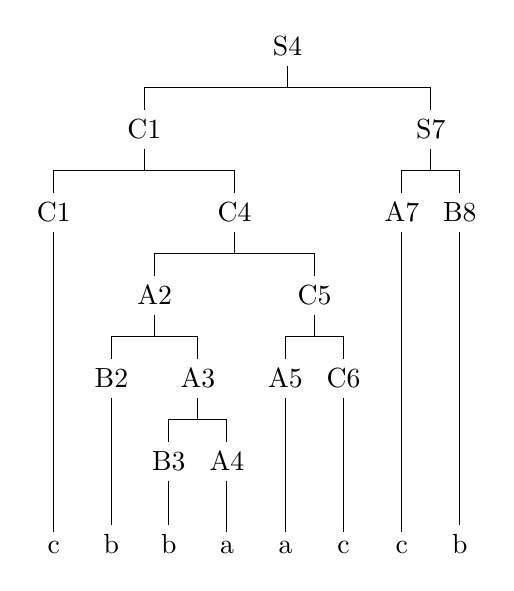
\begin{tikzpicture}[baseline]
		\tikzset{frontier/.style={distance from root=180pt}} %height of tree times 30pt
\tikzset{edge from parent/.style= {
		draw,
		edge from parent path={(\tikzparentnode.south)	-- +(0,-8pt)-| (\tikzchildnode)}
	}
}
\Tree
[.S4
[.C1
[.C1 c ]
[.C4
[.A2
[.B2 b ]
[.A3
[.B3 b ]
[.A4 a ]
]
]
[.C5
[.A5 a ]
[.C6 c ]
]
]
]
[.S7
[.A7 c ]
[.B8 b ]
]
]
		\end{tikzpicture}
}
\end{center}

\pagebreak
\subsection{Overview - UML}


UML-Diagramm showing the general idea of the implementation.\\
List noteworthy used libraries here, too.\\
Maybe some information out of the statistics tool of IntelliJ.

\subsubsection{UML: More Detail 1}
\subsubsection{UML: More Detail 2}

\pagebreak
\subsection{User Interaction}

\noindent Here the specific must can do's are explained with short examples.
\subsubsection{Use Case 1}
\subsubsection{Use Case i}

\pagebreak
	
	\onecolumn
	% einfacher Zeilenabstand
	\singlespacing
	% Literaturliste soll im Inhaltsverzeichnis auftauchen
	%\addcontentsline{toc}{section}{Literaturverzeichnis}
	% Literaturverzeichnis anzeigen
	%\renewcommand\refname{Literaturverzeichnis}
	%\bibliography{Hauptdatei}
	
	%% Index soll Stichwortverzeichnis heissen
	% \newpage
	% % Stichwortverzeichnis soll im Inhaltsverzeichnis auftauchen
	% \addcontentsline{toc}{section}{Stichwortverzeichnis}
	% \renewcommand{\indexname}{Stichwortverzeichnis}
	% % Stichwortverzeichnis endgueltig anzeigen
	% \printindex
	
	\onehalfspacing
	
	% evtl. Anhang
	%\newpage
	%\addcontentsline{toc}{section}{Listings}
	%\fancyhead[L]{Listings} %Kopfzeile links
	%\section*{Listings}

Following are some interesting classes referenced in the thesis that were too long to fit into the text.
\\

\noindent
\textbf{Transaction}:\\
This class is the simple Transaction representation used to control index changes. It is not intended to be similar to a RDBMS transaction, but is merely a batch context with simple commit and rollback features.
\\
\lstset{language=java}
\begin{lstlisting}[frame=htrbl, caption={the simple Transaction contract}, label={lst:Transaction.java}]
public class Transaction implements TransactionContext {

	private boolean progress = true;
	private List<Synchronization> syncs = new ArrayList<>();
	
	@Override
	public boolean isTransactionInProgress() {
		return this.progress;
	}
	
	@Override
	public Object getTransactionIdentifier() {
		return this;
	}
	
	@Override
	public void registerSynchronization(
		Synchronization synchronization ) {
		this.syncs.add( synchronization );
	}
	
	/**
	 * @throws IllegalStateException if already commited/rolledback
	 */
	public void commit() {
		if ( !this.progress ) {
			throw new IllegalStateException( 
			"can't commit - " + 
			"No Search Transaction is in Progress!" );
		}
		this.progress = false;
		this.syncs.forEach( Synchronization::beforeCompletion );
		
		for ( Synchronization sync : this.syncs ) {
			sync.afterCompletion( Status.STATUS_COMMITTED );
		}
	}
	
	/**
	 * @throws IllegalStateException if already commited/rolledback
 	 */
	public void rollback() {
		if ( !this.progress ) {
			throw new IllegalStateException( 
			"can't rollback - " + 
			"No Search Transaction is in Progress!" );
		}
		this.progress = false;
		this.syncs.forEach( Synchronization::beforeCompletion );
	
		for ( Synchronization sync : this.syncs ) {
			sync.afterCompletion( Status.STATUS_ROLLEDBACK );
		}
	}

}
\end{lstlisting}

\pagebreak

\noindent
\textbf{StandaloneSearchConfiguration}:\\
hibernate-search-engine requires an object implementing the SearchConfiguration interface. StandaloneSearchConfiguration is the basic implementation of this used in our standalone version of Hibernate Search.
\\
\lstset{language=java}
\begin{lstlisting}[frame=htrbl, caption={StandaloneSearchConfiguration.java}, label={lst:StandaloneSearchConfiguration.java}]
/**
 * Manually defines the configuration. 
 * Classes and properties are the only implemented options at the moment.
 *
 * @author Martin Braun (adaption), Emmanuel Bernard
 */
public class StandaloneSearchConfiguration 
	extends SearchConfigurationBase 
	implements SearchConfiguration {

	private final Logger LOGGER = 
		Logger.getLogger( 
			StandaloneSearchConfiguration.class.getName() 
		);
		
	private final Map<String, Class<?>> classes;
	private final Properties properties;
	private final HashMap<Class<? extends Service>, Object> 
		providedServices;
	private final InstanceInitializer initializer;
	private SearchMapping programmaticMapping;
	private boolean transactionsExpected = true;
	private boolean indexMetadataComplete = true;
	private boolean idProvidedImplicit = false;
	private ClassLoaderService classLoaderService;
	private ReflectionManager reflectionManager;

	public StandaloneSearchConfiguration() {
		this( new Properties() );
	}

	public StandaloneSearchConfiguration(Properties properties) {
		this( 
			SubClassSupportInstanceInitializer.INSTANCE, 
			properties
		);
	}

	public StandaloneSearchConfiguration(InstanceInitializer init) {
		this( new Properties() );
	}

	public StandaloneSearchConfiguration(InstanceInitializer init, 
		Properties properties) {
		this.initializer = init;
		this.classes = new HashMap<>();
		this.properties = properties;
		// default values if nothing was explicitly set
		this.properties.computeIfAbsent(
			"hibernate.search.default.directory_provider", 
			(key) -> {
				LOGGER.info( 
				  "defaulting to RAM directory-provider" 
				);
			return "ram";
		});
		this.properties.computeIfAbsent(
			"hibernate.search.lucene_version", 
			(key) -> {
				LOGGER.info( 
					"defaulting to Lucene Version: " 
					+ Version.LUCENE_5_2_1.toString() 
				);
				return Version.LUCENE_5_2_1.toString();
		});
		this.reflectionManager = new JavaReflectionManager();
		this.providedServices = new HashMap<>();
		this.classLoaderService = new DefaultClassLoaderService();
	}

	public StandaloneSearchConfiguration addProperty(String key,
		String value) {
		properties.setProperty( key, value );
		return this;
	}

	public StandaloneSearchConfiguration addClass(Class<?> indexed) {
		classes.put( indexed.getName(), indexed );
		return this;
	}

	@Override
	public Iterator<Class<?>> getClassMappings() {
		return classes.values().iterator();
	}

	@Override
	public Class<?> getClassMapping(String name) {
		return classes.get( name );
	}

	@Override
	public String getProperty(String propertyName) {
		return properties.getProperty( propertyName );
	}

	@Override
	public Properties getProperties() {
		return properties;
	}

	@Override
	public ReflectionManager getReflectionManager() {
		return this.reflectionManager;
	}

	@Override
	public SearchMapping getProgrammaticMapping() {
		return programmaticMapping;
	}

	public StandaloneSearchConfiguration setProgrammaticMapping(
			SearchMapping programmaticMapping
		) {
		this.programmaticMapping = programmaticMapping;
		return this;
	}

	@Override
	public Map<Class<? extends Service>, Object> 
		getProvidedServices() {
		return providedServices;
	}

	public void addProvidedService(
			Class<? extends Service> serviceRole,
			Object service
		) {
		providedServices.put( serviceRole, service );
	}

	@Override
	public boolean isTransactionManagerExpected() {
		return this.transactionsExpected;
	}

	public void setTransactionsExpected(
			boolean transactionsExpected) {
		this.transactionsExpected = transactionsExpected;
	}

	@Override
	public InstanceInitializer getInstanceInitializer() {
		return initializer;
	}

	@Override
	public boolean isIndexMetadataComplete() {
		return indexMetadataComplete;
	}

	public void setIndexMetadataComplete(
		boolean indexMetadataComplete) {
		this.indexMetadataComplete = indexMetadataComplete;
	}

	@Override
	public boolean isIdProvidedImplicit() {
		return idProvidedImplicit;
	}

	public StandaloneSearchConfiguration 
		setIdProvidedImplicit(boolean idProvidedImplicit) {
		this.idProvidedImplicit = idProvidedImplicit;
		return this;
	}

	@Override
	public ClassLoaderService getClassLoaderService() {
		return classLoaderService;
	}

	public void setClassLoaderService(
		ClassLoaderService ) {
		this.classLoaderService = classLoaderService;
	}

}
\end{lstlisting}

\pagebreak

\noindent
\textbf{BasicEntityProvider}:\\
This is the basic implementation of the EntityProvider interface which is used to abstract the database access in the standalone version. It uses a JPA EntityManager to accomplish this.
\\
\lstset{language=java}
\begin{lstlisting}[frame=htrbl, caption={BasicEntityProvider.java}, label={lst:BasicEntityProvider.java}]
public class BasicEntityProvider implements EntityProvider {

	private static final String QUERY_FORMAT = 
		"SELECT obj FROM %s obj " +
		"WHERE obj.%s IN :ids";
	private final EntityManager em;
	private final Map<Class<?>, String> idProperties;

	public BasicEntityProvider(EntityManager em,
		Map<Class<?>, String> idProperties) {
		this.em = em;
		this.idProperties = idProperties;
	}

	@Override
	public void close() throws IOException {
		this.em.close();
	}

	@Override
	public Object get(Class<?> entityClass, Object id,
		Map<String, String> hints) {
		return this.em.find( entityClass, id );
	}

	@SuppressWarnings({"rawtypes", "unchecked"})
	@Override
	public List getBatch(Class<?> entityClass, List<Object> ids,
		Map<String, String> hints) {
		List<Object> ret = new ArrayList<>( ids.size() );
		if ( ids.size() > 0 ) {
			String idProperty = 
				this.idProperties.get( entityClass );
			String queryString = 
				String.format(
					QUERY_FORMAT,
					this.em.getMetamodel()
						.entity( entityClass )
						.getName(),
					idProperty
		);
		Query query = this.em.createQuery( queryString );
		query.setParameter( "ids", ids );
			ret.addAll( query.getResultList() );
		}
		return ret;
	}
	
	public void clearEm() {
		this.em.clear();
	}

	public EntityManager getEm() {
		return this.em;
	}

}
\end{lstlisting}

\pagebreak

\noindent
\textbf{Obtaining the idProperties}:\\
This code snippet shows how the idProperties map needed for the instantiation of a BasicEntityProvider can be obtained. This mechanism is used on some other places of Hibernate Search GenericJPA as well.
\\
\lstset{language=java}
\begin{lstlisting}[frame=htrbl, caption={Obtaining idProperties}, label={lst:idProperties.java}]
SearchConfiguration config = ...;

MetadataProvider metadataProvider = 
	MetadataUtil.getDummyMetadataProvider( config );
MetadataRehasher rehasher = new MetadataRehasher();

List<RehashedTypeMetadata> rehashedTypeMetadatas = new ArrayList<>();
for ( Class<?> indexRootType : this.getIndexRootTypes() ) {
	RehashedTypeMetadata rehashed = 
		rehasher.rehash( 
			metadataProvider
				.getTypeMetadataFor( indexRootType ) 
		);
	rehashedTypeMetadatas.add( rehashed );
}

Map<Class<?>, String> idProperties = 
	MetadataUtil.calculateIdProperties( rehashedTypeMetadatas );
\end{lstlisting}

\pagebreak

\noindent
\textbf{MultiQueryAccess}:\\
This is the utility class used to scroll results from multiple queries at once while retrieving the events from the database in the asynchronous approach.
\\
\lstset{language=java}
\begin{lstlisting}[frame=htrbl, caption={MultiQueryAccess.java}, label={lst:MultiQueryAccess.java}]
/**
 * Utility class that allows you to access multiple JPA queries at once.
 * Data is retrieved from the database in batches
 * and ordered by a given comparator.
 * No need for messy Unions on the database level! <br>
 * <br>
 * This is particularly useful if you scroll all the data 
 * from the database incrementally and if you can 
 * compare in Code.
 *
 * @author Martin
 */
public class MultiQueryAccess {

	private final Map<String, Long> currentCountMap;
	private final Map<String, Query> queryMap;
	private final Comparator<ObjectIdentifierWrapper> comparator;
	private final int batchSize;
	
	private final Map<String, Long> currentPosition;
	private final Map<String, LinkedList<Object>> values;
	
	private Object scheduled;
	private String identifier;


	public MultiQueryAccess(
		Map<String, Long> countMap,
		Map<String, Query> queryMap,
		Comparator<ObjectIdentifierWrapper> comparator,
		int batchSize) {
		if ( countMap.size() != queryMap.size() ) {
			throw new IllegalArgumentException( 
				"countMap.size() must be equal " + 
					"to queryMap.size()" );
		}
		this.currentCountMap = countMap;
		this.queryMap = queryMap;
		this.comparator = comparator;
		this.batchSize = batchSize;
		this.currentPosition = new HashMap<>();
		this.values = new HashMap<>();
		for ( String ident : queryMap.keySet() ) {
			this.values.put( ident, new LinkedList<>() );
			this.currentPosition.put( ident, 0L );
		}
	}

	private static int toInt(Long l) {
		return (int) (long) l;
	}

	/**
	 * increments the value to be returned by {@link #get()}
	 *
	 * @return true if there is a value left to be visited 
	 *	in the database
	 */
	public boolean next() {
	
	/*
	 *
	 *
	 * indentation broken to make this readable
	 *
	 *
	 */
	
this.scheduled = null;
this.identifier = null;
List<ObjectIdentifierWrapper> tmp =
	new ArrayList<>( this.queryMap.size() );

for ( Map.Entry<String, Query> entry : this.queryMap.entrySet() ) {
	String identifier = entry.getKey();
	Query query = entry.getValue();
	if ( !this.currentCountMap.get( identifier ).equals( 0L ) ) {
		if ( this.values.get( identifier ).size() == 0 ) {
			// the last batch is empty. get a new one
			Long processed = 
				this.currentPosition.get( identifier );
			// yay JPA...
			query.setFirstResult( toInt( processed ) );
			query.setMaxResults( this.batchSize );
			@SuppressWarnings("unchecked")
			List<Object> list = query.getResultList();
			this.values.get( identifier ).addAll( list );
		}
		Object val = this.values.get( identifier ).getFirst();
		tmp.add( new ObjectIdentifierWrapper( val, identifier ) );
	}
}
tmp.sort( this.comparator );
if ( tmp.size() > 0 ) {
	ObjectIdentifierWrapper arr = tmp.get( 0 );
	this.scheduled = arr.object;
	this.identifier = arr.identifier;
	this.values.get( this.identifier ).pop();
	Long currentPosition = this.currentPosition.get( arr.identifier );
	Long newCurrentPosition = 
		this.currentPosition
			.computeIfPresent( arr.identifier, 
				(clazz, old) -> old + 1 );
	if ( Math.abs( newCurrentPosition - currentPosition ) != 1L ) {
		throw new AssertionFailure( 
			"the new currentPosition count " + 
			"should be exactly 1 " +
			"greater than the old one" );
	}
	Long count = this.currentCountMap.get( arr.identifier );
	Long newCount = this.currentCountMap.computeIfPresent(
		arr.identifier, (clazz, old) -> old - 1
	);
	if ( Math.abs( count - newCount ) != 1L ) {
		throw new AssertionFailure( 
			"the new old remaining count " + 
				should be exactly 1 " +
				"greater than the new one" );
	}
}
return this.scheduled != null;
}

	/**
	* @return the current value
	*/
	public Object get() {
		if ( this.scheduled == null ) {
			throw new IllegalStateException(
				"either empty or next() has " + 
					"not been called" );
		}
		return this.scheduled;
	}

	/**
	* @return the identifier of the current value
	*/
	public String identifier() {
		if ( this.identifier == null ) {
			throw new IllegalStateException( 
				"either empty or next() has " + 
					"not been called" );
		}
		return this.identifier;
	}

	public static class ObjectIdentifierWrapper {
	
		public final Object object;
		public final String identifier;
		
		public ObjectIdentifierWrapper(Object object,
			String identifier) {
			this.object = object;
			this.identifier = identifier;
		}
	
	}

}
\end{lstlisting}

\pagebreak

~
	
	%\newpage
	%\addcontentsline{toc}{section}{Tables}
	%\fancyhead[L]{Tables}
	%\section*{Tables}
This section contains all tables referenced in this thesis.
\\

\noindent
\textbf{JPASearchFactoryController configuration}:\\
When instantiating the JPASearchFactoryController with the Setup class the developer has to pass a property-Map (or a Java Properties) object. Besides containing the hibernate-search-engine configuration properties, some Hibernate Search GenericJPA configuration properties can be set in this map as well:
\\
\begin{table}[h] 
	\centering
	\begin{tabular}{|c|c|}
		\hline 
		hibernate.search.useJTATransactions & \specialcell{ \textbf{false} \\ true } \\ 
		\hline 
		hibernate.search.searchfactory.type & \specialcell{ \textbf{sql} \\ manual-updates  \\ eclipselink \\ hibernate \\ openjpa} \\ 
		\hline
		hibernate.search.trigger.batchSizeForUpdates & \specialcell{ \textbf{5} } \\
		\hline
		hibernate.search.trigger.batchSizeForUpdateQueries & \specialcell{ \textbf{20} } \\
		\hline
		hibernate.search.trigger.updateDelay & \specialcell{ \textbf{200} } \\
		\hline
		hibernate.search.trigger.source & \specialcell{ <class> } \\
		\hline
		hibernate.search.additionalIndexedTypes & \specialcell{ <class>,<class>,... } \\
		\hline
		hibernate.search.transactionManagerProvider & \specialcell{
			\textbf{org.hibernate.}\\\textbf{search.generic}\\\textbf{jpa.trans}\\\textbf{action.impl}\\
			\textbf{JNDILookup}\\\textbf{Transaction}\\\textbf{ManagerProvider} 
		} \\
		\hline
		hibernate.search.transactionManagerProvider.jndi & \specialcell{ <jndi-string> } \\
		\hline
		hibernate.search.trigger.createstrategy & \specialcell{
			\textbf{create} \\
			create-drop \\
			dont-create
		} \\
		\hline
	\end{tabular}
	\footnotesize \caption{Basic JPASearchFactoryController configuration properties (\textbf{default})}
	\label{table:config_properties_jpasearchfactorycontroller}
\end{table}

\pagebreak
~
	
	%\newpage
	%\addcontentsline{toc}{section}{References}
	%\fancyhead[L]{References}
	%%
% ---- Bibliography ----
%
\begin{thebibliography}{100}
	
	\bibitem{jsr_jpa1} JSR 220: Enterprise Java Beans 3.0
	\url{https://jcp.org/en/jsr/detail?id=220}, 09/09/2015
	%
	
	\bibitem{javaworld_jpa1} Javaworld: Understanding JPA, Part 1
	\url{http://www.javaworld.com/article/2077817/java-se/understanding-jpa-part-1-the-object-oriented-paradigm-of-data-persistence.html}, 09/09/2015
	
	\bibitem{hibernate_orm} Hibernate ORM project homepage
	\url{http://hibernate.org/orm/}, 09/09/2015
	
	\bibitem{hibernate_search_homepage} Hibernate Search project homepage
	\url{http://hibernate.org/search/}, 09/09/2015
	
	\bibitem{hsearch_source_code_git} Hibernate Search GitHub repository
	\url{https://github.com/hibernate/hibernate-search}, 09/09/2015
	
	\bibitem{hibernate_search_faq} Hibernate Search FAQ
	\url{http://hibernate.org/search/faq/}, 09/09/2015
	
	\bibitem{lucene_apache_org} Lucene Website
	\url{https://lucene.apache.org/core/}, 09/09/2015
	
	\bibitem{elasticsearch_java_api} ElasticSearch Java API
	\url{https://www.elastic.co/guide/en/elasticsearch/client/java-api/current/index.html}, 09/09/2015
	
	\bibitem{solr_java_api} Solr Java API
	\url{https://wiki.apache.org/solr/Solrj}, 09/09/2015
	
	\bibitem{xkcd_competing_standards_source} xkcd \#927 on competing standards
	\url{https://xkcd.com/927/}, 09/09/2015
	
	\bibitem{top_down_strandh} Top-down programming, Robert Strandh
	\url{http://dept-info.labri.fr/~strandh/Teaching/PFS/Common/Strandh-Tutorial/top-down-programming.html},
	09/09/2015
	
	\bibitem{bottom_up_strandh} Bottom-up programming, Robert Strandh
	\url{http://dept-info.labri.fr/~strandh/Teaching/PFS/Common/Strandh-Tutorial/bottom-up-programming.html},
	09/09/2015
	
	\bibitem{singleresponsibility_objectmentor} objectmentor.com: Article on Single Responsibility Principle
	\url{http://www.objectmentor.com/resources/articles/srp.pdf}, 09/09/2015
	
	\bibitem{openclosed_objectmentor} objectmentor.com: Article on Open-Closed-Principle
	\url{http://www.objectmentor.com/resources/articles/ocp.pdf}, 09/09/2015
	
	\bibitem{openclosed_bertrand} Object-Oriented Software Construction, Prentice Hall, 1988, Bertrand Meyer
	
	\bibitem{maven_homepage} Maven project homepage
	\url{https://maven.apache.org/}, 09/09/2015
	
	\bibitem{jdbc_oracle} Oracle JDBC overview
	\url{http://www.oracle.com/technetwork/java/javase/jdbc/index.html}, 09/09/2015
	
	\bibitem{oledb_ms} Documentation on how to use OleDb with .NET
	\url{https://msdn.microsoft.com/en-us/library/5ybdbtte(v=vs.71).aspx}, 09/09/2015
	
	\bibitem{wikibooks_on_jpa} Wikibooks on Java Persistence
	\url{https://en.wikibooks.org/wiki/Java_Persistence/What_is_JPA\%3F}, 09/09/2015
	
	\bibitem{stackoverflow_jpa} Stackoverflow JPA tag
	\url{http://stackoverflow.com/tags/jpa/info}, 09/09/2015
	
	\bibitem{hibernate_ogm} Hibernate OGM project homepage
	\url{http://hibernate.org/ogm/}, 09/09/2015
	
	\bibitem{eclipselink} EclipseLink project homepage
	\url{http://www.eclipse.org/eclipselink/}, 09/09/2015
	
	\bibitem{jpa_21_jcp} JSR 338: JPA 2.1 specification
	\url{https://jcp.org/en/jsr/detail?id=338}, 09/09/2015
	
	\bibitem{openjpa} OpenJPA project homepage
	\url{http://openjpa.apache.org/}, 09/09/2015
	
	\bibitem{java_ee_spec} Java EE specification on oracle.com
	\url{http://www.oracle.com/technetwork/java/javaee/tech/index.html}, 09/09/2015
	
	\bibitem{sql_like_w3schools} w3schools on SQL LIKE
	\url{http://www.w3schools.com/sql/sql_like.asp}, 09/09/2015
	
	\bibitem{lucene_basic_concepts} Lucene Tutorial
	\url{http://www.lucenetutorial.com/basic-concepts.html}, 09/09/2015
	
	\bibitem{elasticsearch_homepage} ElasticSearch Homepage
	\url{https://www.elastic.co/products/elasticsearch}, 09/09/2015
	
	\bibitem{solr_homepage} Solr Homepage
	\url{http://lucene.apache.org/solr/}, 09/09/2015
	
	\bibitem{elasticsearch_downloads_website} ElasticSearch Download website
	\url{https://www.elastic.co/downloads/elasticsearch}, 09/09/2015
	
	\bibitem{solr_security} Solr security
	\url{https://wiki.apache.org/solr/SolrSecurity}, 09/09/2015
	
	\bibitem{elasticsearch_security} elastic Shield (security for ElasticSearch)
	\url{https://www.elastic.co/products/shield}, 09/09/2015
	
	\bibitem{solr_admin} Solr Administration (Core Specific Tools)
	\url{https://cwiki.apache.org/confluence/display/solr/Core-Specific+Tools}, 09/09/2015
	
	\bibitem{elasticsearch_admin} ElasticHQ
	\url{http://www.elastichq.org/}, 09/09/2015
	
	\bibitem{elasticsearch_clustering} ElasticSearch: Life inside a cluster
	\url{https://www.elastic.co/guide/en/elasticsearch/guide/current/distributed-cluster.html}, 09/09/2015
	
	\bibitem{solr_clustering} Solr: Introduction to Scaling and Distribution
	\url{https://cwiki.apache.org/confluence/display/solr/Introduction+to+Scaling+and+Distribution}, 09/09/2015
	
	\bibitem{hibernate_search_engine_mvnrepository} hibernate-search-engine on mvnrepository.org
	\url{http://mvnrepository.com/artifact/org.hibernate/hibernate-search-engine/5.4.0.Final}, 09/09/2015
	
	\bibitem{hibernate_search_roadmap} Hibernate Search roadmap
	\url{http://hibernate.org/search/roadmap/}, 09/09/2015
	
	\bibitem{hibernate_search_javadoc} Hibernate Search JavaDoc
	\url{https://docs.jboss.org/hibernate/search/5.5/api/}, 09/09/2015
	
	\bibitem{hibernate_search_doc} Hibernate Search documentation
	\url{http://hibernate.org/search/documentation/}, 09/09/2015
	
	\bibitem{hibernate_search_doc_massindexer} Hibernate Search documentation (MassIndexer, v5.4)
	\url{https://docs.jboss.org/hibernate/search/5.4/reference/en-US/html_single/#search-batchindex-massindexer}, 09/09/2015
	
	\bibitem{mysql_developers_lib} MySQL - Developer's Library, Fourth Edition, 2009, Paul DuBois
	
	\bibitem{postgres_triggers} CREATE TRIGGER in PostgreSQL
	\url{http://www.postgresql.org/docs/9.1/static/sql-createtrigger.html}, 09/09/2015
	
	\bibitem{hsqldb_triggers} Triggers in HSQLDB
	\url{http://hsqldb.org/doc/guide/triggers-chapt.html}, 09/09/2015
	
	\bibitem{firebird_triggers} Triggers in Firebird
	\url{http://www.firebirdsql.org/refdocs/langrefupd21-ddl-trigger.html}, 09/09/2015
	
	\bibitem{postgres_truncate} Truncate statement PostgreSQL docs
	\url{http://www.postgresql.org/docs/9.1/static/sql-truncate.html}, 09/09/2015
	
	\bibitem{firebird_conformance} Firebird conformance
	\url{http://www.firebirdsql.org/en/sql-conformance/}, 09/09/2015
	
	\bibitem{hibernate_genericjpa_github} Hibernate Search GenericJPA GitHub repository
	\url{https://github.com/Hotware/Hibernate-Search-GenericJPA}, 09/09/2015
	
	
\end{thebibliography}
	
	
	\bibliography{literature}{}
	\bibliographystyle{unsrt}
	
	\newpage
	% Erklärung
	\addcontentsline{toc}{section}{Erklärung}
	\fancyhead[L]{Erklärung}
	\section*{Erklärung}

\begin{verbatim}

\end{verbatim}

\noindent
\begin{LARGE}Erklärung zur Bachelorarbeit\end{LARGE}
\begin{verbatim}


\end{verbatim}
Ich versichere, die von mir vorgelegte Arbeit selbstständig verfasst zu haben. Alle Stellen, die wörtlich oder sinngemäß aus veröffentlichten oder nicht veröffentlichten Arbeiten anderer entnommen sind, habe ich als entnommen kenntlich gemacht. Sämtliche Quellen und Hilfsmittel, die ich für die Arbeit benutzt habe, sind angegeben. Die Arbeit hat mit gleichem Inhalt bzw. in wesentlichen Teilen noch keiner anderen Prüfungsbehörde vorgelegen.



\begin{displaymath}
% use packages: array
\begin{array}{ll}
Unterschrift:~~~~~~~~~~~~~~~~~~~~~~~~~~~~~~~~~~~~~~~~~~
& Ort, Datum:~~~~~~~~~~~~~~~~~~~~~~~~~~~~~~~~~~~~~~~~~~
\end{array}
\end{displaymath}

	
	% leere Abschlussseite
	%\newpage
	%\thispagestyle{empty} % erzeugt Seite ohne Kopf- / Fusszeile
	\section*{ }
	
\end{document}